\documentclass[10pt,a4paper]{article}
\usepackage[margin=2.2cm]{geometry}
\usepackage[T1]{fontenc}
\usepackage{lmodern}
\usepackage{microtype}
\DisableLigatures[-]{encoding = T1, family = tt*}   % --options in \code stay two hyphens, not an en dash
\usepackage{graphicx}
\usepackage{booktabs}
\usepackage{array}
\usepackage{amsmath}
\usepackage{xcolor}
\usepackage{listings}
\usepackage{enumitem}
\usepackage{float}
\usepackage{xurl}   % long URLs in the bibliography may break at any character
\usepackage[hidelinks]{hyperref}
\setlist{nosep, leftmargin=1.4em}
\renewcommand{\arraystretch}{1.12}
\newcommand{\code}[1]{\texttt{\small #1}}
\newcommand{\MC}{MC/s}
\newcommand{\repourl}{\url{https://github.com/anmartinez1256/emsKit}}   % the repository URL, set once, here
\lstset{basicstyle=\ttfamily\footnotesize, breaklines=true, columns=fullflexible, keepspaces=true,
  frame=single, framerule=0.2pt, rulecolor=\color{gray!50}, xleftmargin=4pt, xrightmargin=4pt, aboveskip=4pt, belowskip=6pt}
\graphicspath{{figures/}}

\title{\vspace{-1cm}fdtdKit: taking openEMS towards the memory ceiling of an Apple~M5\\
\large A bit-identical speed-up of the EC-FDTD engine, and two run-length levers on the modelling side}
\author{Angel Martinez\\ University of Texas at Austin}
\date{Work of 2026-10-28 to 2026-11-13; draft of 2026-11-13}
% PDF metadata: keep pdfauthor in step with the name in \author
\hypersetup{pdftitle={fdtdKit: taking openEMS towards the memory ceiling of an Apple M5}, pdfauthor={Angel Martinez}}

\begin{document}
\sloppy
\maketitle
\vspace{-0.6cm}

\begin{abstract}
openEMS is a free electromagnetic field solver that uses the equivalent-circuit finite-difference time-domain
(EC-FDTD) method. On an Apple M5 laptop its multithreaded CPU engine ran the four models of up to about a million cells
studied here (two openEMS tutorials and two printed-circuit boards) at 268--379 million cell updates per second (\MC;
its best of 2, 4 and 8 threads), well below the roughly 2\,000\,\MC\ that the machine's 153\,GB/s of unified memory
allows at the 74 bytes per cell and time step of our traffic model. We report changes to the CPU engine that bring the
same models to 1\,808--1\,961\,\MC, 4.73--6.89$\times$ the speed of stock v0.37.0 built with Apple clang, and two
refined tutorial models of 5--8 million cells to 1.95--2.72$\times$ (snapshot cg29 of 2026-11-05, paired with stock in
the same rounds; on the patch tutorial the fork's base alone, with upstream's background dump writer, ran 1.13$\times$
as fast as stock in separate runs of 2026-11-03), with results identical bit for bit to stock for the same number of
time steps; changes to the operator setup
and the far-field post-processing that cut their times (4.1\,s to 0.9\,s and 17.9\,s to 1.0\,s on a 7.9-million-cell
model; from the project log); an opt-in Metal engine that advances tiles of the grid several time steps at a time (the
diamond tile schedule of luikore's openEMS pull request \#228, without its code), identical bit for bit to the CPU
engine when the CPU, like the GPU, flushes subnormal numbers; and two changes on the modelling side (a run-end
criterion based on the port probes, and a mesh-line merging rule with a minimum cell size) that shorten the runs
themselves. In the same paired runs the Metal engine ran the two large models at 2\,879 and 3\,193\,\MC, 1.47 and
1.46$\times$ the CPU engine at its best, and one board, a grounded-coplanar (GCPW) line, 1.17$\times$; it was level on
the other, a vertical SMA launch (1.00$\times$, 1.07 million cells), and slower on the two tutorials (0.97 and
0.93$\times$); a later build (cg31, 2026-11-11) raised the Metal engine's rates by 1.07--1.53$\times$ on the six models.
In a sweep of three models over 0.1--7.9 million cells it was ahead in every round from 1.7--2.9
million cells on, depending on the model, by 1.25--1.52$\times$ above 3 million, and within 0.89--1.23$\times$ of the
CPU engine below that. Unblocked, as a fused sweep, it reaches only 67--75\,\% of that sweep's traffic bound on the large
models: on this machine, whose GPU shares the bus with the cores, the blocking carries the gain. Together, the CPU
engine of cg18 (patches 0001--0006, the author's installed build until cg29 replaced it on 2026-11-06) and the
toolkit's defaults since 2026-11-04 cut the solver
time of a complete simulation of the SMA launch from 562.7\,s with stock openEMS to 37.4\,s (15.0$\times$) and that of a
50\,mm GCPW line from 76.5\,s to 5.2\,s (14.7$\times$; 5.8$\times$ and 8.9$\times$ with the toolkit's defaults until
2026-11-04, a 0.02\,mm floor and a hold of 1); with cg29 the Metal engine ran these default runs 1.22 and 1.37$\times$
faster than the CPU engine
(paired per round, on a loaded machine). All these times are measured. We describe the measurement harness and the
verification policy that made this safe, the mechanisms behind each gain (barriers and the neighbour flags that
replaced them, the inner loop, work distribution, a fused E/H sweep that cuts the modelled DRAM traffic from 74 to 49
bytes per cell, an allocation-placement valley, the boundary and dispersive-material paths, coefficient tables, the
GPU's diamond tiles), and what did not work, and repeat the main measurements, as a set of their own, on a second
machine, an M5 Pro Mac mini, where the CPU engine of cg31 runs 2.7 to 14.1$\times$ as fast as stock at stock's best thread
count, and time three later patches (0041 to 0043) there, with a paired comparison against upstream master's new CPU engine
(ahead at 1~million cells, level to 14\,\% ahead at 8~million on empty and PML grids (0.93$\times$ on the PML grid at 5 threads), behind on an 8-million-cell dispersive case). Because on the M5 the memory bus of one machine bounds the cell rate on large grids (on the M5 Pro it held back only the largest grid
measured, 16.8~million cells), we also
outline, without measurements, how a domain-decomposed engine (openEMS has none today) could spread one model over a
Thunderbolt-connected cluster of Mac mini or Mac Studio machines, each adding its own unified memory and bus. The
engine patches, the benchmark harness, the result tables, the scripts and a command line that runs the harness and
the checks (\code{emskit fdtd}) are published at \repourl.
\end{abstract}

\section{Introduction}

openEMS~\cite{liebig2013} is a widely used free finite-difference time-domain (FDTD)~\cite{yee1966,taflove} solver.
The author runs it from a Python toolkit for printed-circuit-board RF work: 50\,$\Omega$ grounded-coplanar waveguide
(GCPW) lines with lossy conducting sheets, vertical and edge-mount SMA (SubMiniature version A) connector launches with
a coaxial port and a perfectly matched layer (PML), coupled lines and cavities. The machine is an Apple M5 laptop (4
performance and 6 efficiency cores, 16\,GB of unified memory on a single bus of about 150\,GB/s~\cite{m5}, shared with
the GPU). A survey of the toolkit's runs on it found 0.1--2.4 million cells, 41\,000--165\,000 time steps and 10--50
minutes per run at 117--460 million cell updates per second (\MC; from the project log, not in \code{results/}). The
two boards benchmarked here take 76.5\,s and 562.7\,s per full run with stock openEMS (measured,
Table~\ref{tab:e2e}). A parameter study of a launch footprint is a day.

The question this work set out to answer was simply ``how fast can openEMS go on this machine, without changing its
answers?'' The constraint matters: the solver is used as a design gate, its results are compared to measurements and
to earlier runs, and a fast engine that moves the answer by a tenth of a decibel is a liability, not an asset. Every
change to the solver reported here therefore had to reproduce the stock engine's port voltages and currents,
S-parameters and field dumps to the bit for the same number of time steps (the two exceptions, the GPU engines, as
Apple's GPU flushes subnormal numbers to zero, and a float accumulation order in the far-field transform, are called
out where they appear; the fork's own Metal engine is held to the bit against the CPU engine run with the same flush).
These changes make up a fork of openEMS, which together with the benchmark harness and the verification method used
to build it is called fdtdKit (emsKit until 2026-11-05, the name its repository keeps; Section~\ref{sec:repro}).
fdtdKit is the FDTD kit of EMSKit, a family of electromagnetic solvers for Apple silicon; the family's other kits
(femKit, momKit and sbrKit) are not part of this report.

\paragraph{Contributions.}
\begin{itemize}
\item A benchmark harness that runs the stock and the modified engines in-process on the same models with a fixed
  number of time steps, waits for a quiet machine, and compares port probes and S-parameters bit for bit; HDF5 field
  dumps are compared dataset by dataset with \code{scripts/checks/h5cmp.py} (Section~\ref{sec:method}).
\item A sequence of engine changes, each measured and verified on six models (Section~\ref{sec:engine}): thread
  barriers and a per-extension hook plan, a rewritten inner loop, work stealing and an automatic thread count, vector
  paths for the Mur and uniaxial-PML (UPML) boundaries, a fused E/H sweep that lowers the modelled DRAM traffic from
  74 to 49 bytes per cell, the SSE engines' use of upstream's precomputed dump gather, staggered allocations that
  avoid an allocation-placement valley, a scalar-SSE path and compressed tables for PML slabs, line hooks for the
  dispersive-material extension, packed coefficient tables, and thread quality-of-service on macOS. Together
  (snapshot cg14, against stock v0.37.0 built with Apple clang): 3.2--6.9$\times$ on the four models of up to about a
  million cells, 1.7--2.5$\times$ on the two of 5--8 million cells, where stock already ran at up to half the bus
  (Section~\ref{sec:background}). On the patch tutorial about 1.13$\times$ of the 6.9$\times$ comes from the fork's
  base, upstream's \code{gpu-engine} branch, whose HDF5 writer writes that model's time-domain dumps in the
  background; on the notch tutorial, the GCPW line and patch x5 the base runs within 0.98--1.03$\times$ of stock
  (Section~\ref{sec:results}). Snapshot cg18 (patches 0001--0006, the build installed on the author's Mac from
  2026-11-04 to 2026-11-06) gives 3.1--6.8$\times$ on the same four models against the stock rows of its check
  tables. Snapshot cg29 (patches 0001--0027, the installed build from 2026-11-06 to 2026-11-11) adds the CPU items
  of a second
  review and ideas from other contributors' work (Section~\ref{sec:cg29}): an operator index per z-vector, neighbour
  flags in place of the two barriers per time step, a y-row path for UPML boxes, merged ADE updates for conducting
  sheets, geometry coefficient tables and line hooks for the steady-state detection and Debye materials. Paired with
  stock in the same rounds (cg29 at 8 threads, its best setting; stock at its best of 2, 4 and 8 threads), it runs
  the four models 4.73--6.89$\times$ and the two large ones 1.95$\times$ and 2.72$\times$ as fast as stock
  (Table~\ref{tab:current}); paired with cg18 in rounds of its own (5 rounds, other processes on 0.3--0.6 cores; the
  SMA launch on its 0.871\,M-cell mesh), 1.03--1.23$\times$ as fast at 4 threads and 1.13--1.44$\times$ at 8 over the
  six models.
\item Setup and post-processing: a threaded operator construction (4.1\,s to 0.9\,s on the 7.9-million-cell patch
  model), a far-field transform written as complex matrix products, one per plane and block of directions (17.9\,s to
  1.0\,s on the same model; this path needs Apple's Accelerate, other builds keep the original loop), and two small
  CSXCAD changes (times from the project log, not in \code{results/}).
\item An analysis of the ceiling (Section~\ref{sec:beyond}). On a $201^3$ box the CPU engine (snapshot cg9, 8 threads),
  upstream's Metal engine from its pre-merge \code{gpu-engine} branch, and a standalone Swift/Metal kernel that runs
  the exported openEMS operator bit-identically reached 1\,562, 1\,638 and 1\,670\,\MC\ (from the project log, not in
  \code{results/}). By the traffic model the two Metal kernels move 74\,B per cell (separate E and H passes) and the
  fused CPU sweep 49\,B, so the GPU drew more of the bus for about the same cell rate; no byte count was measured with
  hardware counters. On all six test models the CPU engine of cg14 and of cg18 is faster than that Metal engine
  (Section~\ref{sec:ceiling}). Upstream master's merged Metal engine and luikore's diamond-blocked one were built and
  run here on 2026-11-04 (Section~\ref{sec:positioning}), and on 2026-11-11 next to cg31 on luikore's benchmark model
  (Table~\ref{tab:threebuilds}).
\item A diamond-blocked Metal engine (\code{--engine=metal-diamond}, opt-in, Apple only; patches 0007--0016,
  Section~\ref{sec:gpu}) that advances tiles of the grid several time steps at a time, with the tile schedule of
  luikore's openEMS pull request \#228~\cite{luikore228} (none of its code is used). All six models run on the GPU,
  identical bit for bit to the multithreaded CPU engine run with \code{OPENEMS\_FTZ=1}; against stock, which keeps
  subnormal numbers, its port probes differ by $1.7\times10^{-7}$ to $9.4\times10^{-7}$ relative. Paired with the CPU
  engine of cg29 at its best (Table~\ref{tab:current}) it runs patch x5 and notch x3 1.47$\times$ and 1.46$\times$ as
  fast and the GCPW line 1.17$\times$, is level on the SMA launch (1.00$\times$, 1.071\,M cells) and slower on the
  notch and patch tutorials (0.97$\times$ and 0.93$\times$). Across grid sizes (Figure~\ref{fig:crossover}) it leads
  in every round from 1.7--2.9 million cells on, depending on the model, and by 1.25--1.52$\times$ above 3 million; on
  smaller grids it waits for the CPU between short calls (the patch tutorial) or runs at a lower rate of its own (the
  notch tutorial), and the CPU engine is at its fastest between 0.6 and 1.9 million cells. Unblocked, as a fused sweep ($K=1$), the Metal engine runs the two large
  models at 1\,730--1\,840\,\MC, only 67--75\,\% of that sweep's traffic bound (cg27, medians of paired rounds with
  2.5--4 cores of other load; \code{results/fused\_sweep\_k1\_2026-11-04.txt}): the blocking carries the gain.
  A later build, cg31 (patches 0028--0039 of 2026-11-11, the installed build since that day), raises the Metal
  engine's rates on the six models by 1.07--1.53$\times$, which puts it ahead of the CPU engine on five of them and
  level on the patch tutorial (Section~\ref{sec:cg31}).
\item Two modelling-side levers (Section~\ref{sec:modelling}): a run-end criterion on the port probes
  (Table~\ref{tab:probeend}; the energy criterion stalls on the static charge left behind by openEMS's Gaussian pulse,
  which has a DC component, so the runs always went to their maximum time; upstream has since added an opt-in DC-free
  pulse, commit d686f1d, which is not in this work's base), and a mesh-line merging rule with a minimum cell size whose
  sweep on the SMA launch gives another 2.0$\times$ for 0.12\,dB of $S_{11}$ at $-23$\,dB (Section~\ref{sec:meshfloor}).
  Since 2026-11-04 the toolkit's defaults use the shorter settings of both (a hold of 0.5 instead of 1; on the SMA
  launch a 0.05\,mm floor instead of 0.02\,mm); together with
  the CPU engine of cg18 they cut a complete simulation of the SMA launch from 562.7\,s with stock to 37.4\,s and one
  of the GCPW line from 76.5\,s to 5.2\,s (Table~\ref{tab:e2e}), and with cg29 the Metal engine ran these runs
  1.22$\times$ and 1.37$\times$ as fast as the CPU engine (Table~\ref{tab:e2ecg29}, paired per round, on a loaded
  machine).
\item A list of things that did not work, with numbers (Section~\ref{sec:rejected}), and the artefact set
  (Section~\ref{sec:repro}).
\end{itemize}

\paragraph{Scope.} All numbers are from one machine, an Apple M5 MacBook with 16\,GB, macOS~27.0.1, Apple clang~21,
except two validation-suite runs made on a Linux virtual machine (Section~\ref{sec:repro}).
They were measured while the machine was also used for other work (the harness reports the load of other processes
with every number: sampled in the second before each run and, since the cg27 tables of 2026-11-04, their CPU and GPU
use during it,
Section~\ref{sec:method}). Stock openEMS and the fork were both built with Apple
clang, the default on macOS; upstream's FAQ~\cite{biergaizi29} advises building openEMS with GCC on macOS because
clang generates inefficient code for the SSE engine. That was measured for the inner loop only, in the standalone
kernel, which holds a copy of the stock loop and of its rewrite (one thread, three grids outside the valley;
\code{results/kernel\_gcc\_vs\_clang\_2026-11-03.txt}): GCC~16 runs the stock loop 1.16--1.39$\times$ faster than
Apple clang, and the rewrite of snapshot AB (Section~\ref{sec:engine}) at about the same speed with both, so against
a GCC-built stock the rewrite's one-thread gain in the kernel is 1.26--1.47$\times$ instead of 1.74--1.80$\times$. In
the same kernel the rewrite gives the stock loop's results bit for bit under clang but not under GCC, which contracts
it differently (Section~\ref{sec:contract}). A GCC build of openEMS itself was not made, so the factors of this paper
are against stock built with Apple clang, the default compiler on macOS, and the bit-identity checks used clang builds.
The synchronisation and hook changes do not depend on the compiler. Five details are platform-specific and guarded:
thread QoS (macOS), the starting point of the automatic thread search (the performance-core count on macOS, half the
available hardware threads elsewhere; since cg29 the flag waits on macOS spin only while the thread count is at most
that count, and other CPUs keep the barrier spin time), the separable far-field path (built only with Apple's
Accelerate; other builds keep the original loop), the opt-in flush-to-zero of subnormals (any arm64 CPU) and the
Metal diamond engine (Apple only, opt-in, built with \code{ENABLE\_METAL}). The fused sweep's mechanism, fewer
passes over the fields, is not specific to this CPU, but it was measured only here. The allocation-placement valley
depends on where the allocator puts the two field arrays and was seen only with the allocator of macOS~27.0.1 on the
M5 (Section~\ref{sec:valley}); the stagger that avoids it is applied on every platform and costs nothing measurable
outside the valley.

\section{Background}\label{sec:background}

\subsection{The EC-FDTD update and its memory traffic}
openEMS stores voltages $v$ (the E-field integrated along a cell edge) and currents $i$ (the H-field integrated along
a dual edge), three components each, as 32-bit floats, and advances them with the usual leap-frog:
\begin{align}
v_n &\leftarrow vv_n\, v_n + vi_n\,(\text{curl of } i \text{ around the edge}), \\
i_n &\leftarrow ii_n\, i_n + iv_n\,(\text{curl of } v \text{ around the dual edge}),
\end{align}
with four coefficients per component and cell. Stock openEMS already keeps the coefficients in a \emph{compressed}
operator (\code{Operator\_SSE\_Compressed} in v0.37.0): \code{f4vector}s of four cells (Section~\ref{sec:engines})
whose coefficients agree lane by lane share one entry of a table, and each \code{f4vector} carries a 32-bit index
into it, 1\,B per cell. The index array itself is allocated with one 32-bit entry per cell, of which one per vector
is used; on meshes with few z lines the unused entries share cache lines with the used ones, so the engine streams up
to the full 4\,B per cell (in stock and in the fork up to cg28; cg29 allocates one entry per z-vector,
Section~\ref{sec:cg29}). The table is small (2\,500--69\,500 entries for the models here, under 14\,MB: 1.5\,MB for
the tutorials, 13\,MB for the SMA launch; from the project log) and largely cache-resident; the per-cell traffic that
remains is the fields themselves. With separate E and H passes, each pass reads and writes its own field (12\,B each
way) and reads the other field (12\,B) from DRAM; with the index that is 37\,B per update and roughly 74 bytes per
cell and time step. This is a traffic model, not a counter measurement, as are all bytes-per-cell figures in this
paper; it counts the compact 1\,B of index, and Section~\ref{sec:engine} also gives the figures with the index as
allocated. At 150\,GB/s, a sweep that moves these 74 bytes per cell from DRAM in every time step runs at
2\,000\,\MC\ at best~\cite{roofline} (an engine that keeps a tile's fields on chip over several time steps moves fewer,
Section~\ref{sec:gpu}); the stock engine's 1\,041\,\MC\ on a 7.9-million-cell model is 77\,GB/s, half the bus.
Smaller models fit in part in a last-level cache
of a few tens of MB and could in principle run faster; stock ran them \emph{slower} (277--318\,\MC), which is the
first hint that something other than bandwidth dominated there.

\subsection{Engines, operators, extensions}\label{sec:engines}
openEMS separates the operator (coefficients and mesh, built once) from the engine (the time loop). The SSE engines
work on \code{f4vector}s, four floats in one 16-byte vector. With $n_v=\lceil N_z/4\rceil$ z-vectors per z-line, one
vector holds the cells $z$, $z+n_v$, $z+2n_v$ and $z+3n_v$; the arrays are stored component-fastest (C order
\code{[x][y][z\_v][component]}, the I-J-K-N layout of Section~\ref{sec:engine}), and the z extent is padded to $4n_v$.
Boundary conditions, excitations, lumped elements, dispersive materials and the cylindrical multigrid are
\emph{extensions}, each with up to six hooks per time step (pre-/apply-/post- for voltages and for currents). The
multithreaded engine splits the x range into one slab per thread and runs each hook of each extension between
barriers.

\subsection{The machine}
Apple M5 (2025): 4 performance (P) and 6 efficiency (E) cores, 16\,GB LPDDR5X unified memory, 153\,GB/s
nominal~\cite{m5}. The GPU has no memory of its own; it competes with the cores for the same bus. We measured the
ceiling with two standalone kernels (a $200^3$ box with perfect-electric-conductor (PEC) walls, no PML; from the
project log, not in \code{results/}): a material-table CPU loop reaches 1\,491\,\MC\ at 72 bytes per cell (107\,GB/s)
and the same kernel in Metal 1\,763\,\MC\ (127\,GB/s). The GPU gets 15--20\,\% more of the bus than the cores, but no
bandwidth of its own. Everything that follows is therefore about moving fewer bytes, fewer times, with fewer stalls.

\section{Method: how speed was measured and correctness enforced}\label{sec:method}

\subsection{Models}
Six models span the sizes and features that matter (Table~\ref{tab:models}). Four are the openEMS Python tutorials,
two of them with the mesh refined (``x5'', ``x3'') to a size that is clearly bandwidth-bound; two are the author's
real boards, built by the author's toolkit. Every feature in daily use is covered: Mur and PML boundaries (full-z slabs
and a z-only slab), lumped, microstrip-line (MSL) and coaxial ports, conducting sheets (the dispersive-material
extension), near-field-to-far-field (nf2ff) dumps, frequency-domain field dumps. The cylindrical multigrid was checked
separately on openEMS's CylindricalWave\_CC tutorial.

\begin{table}[H]\centering\small
\resizebox{\textwidth}{!}{\begin{tabular}{@{}llrl@{}}
\toprule
model & origin & cells & features exercised \\
\midrule
patch tutorial & Simple\_Patch\_Antenna.py & 0.104\,M & lumped port, 6$\times$ MUR, nf2ff box (12 time-domain dumps) \\
notch tutorial & MSL\_NotchFilter.py & 0.270\,M & MSL ports, PML\_8 at both x ends, PEC at $z_{\min}$, MUR elsewhere \\
patch x5 & patch, mesh $\times$5 & 7.86\,M & bandwidth-bound size, MUR \\
notch x3 & notch, mesh $\times$3 & 5.25\,M & bandwidth-bound size, PML slabs \\
GCPW line (kgcpw) & rfsim gcpw\_line & 0.242\,M & conducting sheets (dispersive extension), MSL ports, MUR, 17 z lines \\
SMA launch (ksma) & rfsim sma\_launch & 1.071 / 0.871\,M & coaxial port, z-only PML\_8, 69\,500 / 64\,410 distinct operators, FD dumps \\
\bottomrule
\end{tabular}}
\caption{Benchmark models. ``M'' = million Yee cells. The SMA launch has two meshes: 1.071\,M cells with the
toolkit's former 0.02\,mm mesh floor, the mesh of the benchmark tables up to snapshot cg18, and 0.871\,M with the
0.05\,mm floor that is the toolkit's default since 2026-11-04 (toolkit commit 4a7e20e, Section~\ref{sec:meshfloor}),
on which the benchmark model has been built since then: the GPU engine's
measurements (Section~\ref{sec:gpu}), the other engines' runs (Section~\ref{sec:positioning}), the checks of cg29 and
its comparison with cg18 (\code{results/cpu\_items\_cg29\_2026-11-05.txt}) use it. Tables that use the 1.071\,M mesh
say so. Rates on the two meshes do not compare directly. Operator counts: 69\,500 on the 1.071\,M mesh (project log,
not in \code{results/}), 64\,410 on the 0.871\,M mesh
(\code{results/diamond\_engine\_cg24\_cg27\_2026-11-04.txt}).}\label{tab:models}
\end{table}

\subsection{The harness}
\code{bench.py MODEL --configs CFG...} builds the model in a fresh Python process per run (\code{runner.py}) and calls
\code{FDTD.Run()} with a fixed number of time steps (\code{EndCriteria=0}), so every engine performs identical work. A
configuration names the library to load (\code{SNAP@}, a saved set of \code{libopenEMS}, \code{libCSXCAD},
\code{libnf2ff} dylibs picked up through \code{DYLD\_LIBRARY\_PATH}), the engine, the thread count, and environment
variables for individual knobs (\code{\#NAME=VAL}). The first configuration is the reference; for every other run the
harness reports the maximum relative difference of the port probe files and the largest difference of
$S_{11}$/$S_{21}$ (linear and dB, over the frequencies where $|S_{\rm ref}|>-40$\,dB), the engine speed in \MC\ parsed
from openEMS's own output, and the CPU load of \emph{other} processes in the second before the run (\code{others NN\%},
from \code{top}). A probe file whose reference is all zero, and an $S$-parameter that stays below $-40$\,dB, cannot be
compared that way, and the published tables leave them out without a note: the notch x3 check ends before the pulse
reaches port 2, so its tables compare neither the port-2 probes nor $S_{21}$, and the GCPW tables do not compare
$S_{11}$. \code{--quiet 60} waits until other processes use less than 60\,\% of a core, for at most \code{--quiet-max}
seconds; \code{--repeat 2} runs each configuration twice and reports the faster run (both speeds are listed), and in
the tables in \code{results/} only each configuration's last run was compared. The harness now compares every probe
file and $S$-parameter exactly, over all frequencies, and names those without a figure in its output; it also compares
every run with the reference configuration's first run and flags the reported run when its quiet wait timed out.
Since 2026-11-04 the two GPU engines (\code{gpu}, \code{metal-diamond}) and any configuration with
\code{OPENEMS\_FTZ} set count as tolerant: their differences from a stock reference are printed but do not fail the
run, since neither is bit-identical to a run that keeps subnormal floats (the GPU engines' reference is the CPU
engine run with \code{OPENEMS\_FTZ=1}; Section~\ref{sec:policy}). From the cg27 tables of the same day on, each line
also gives the CPU and GPU use of the other processes during the run (\code{bench/usage.py}), following the author's
rule of that day that every benchmark line carries both. A knob's value cannot contain a comma, because the harness
splits its settings on commas; a tile setting \code{M,V} of the GPU engine was once silently dropped that way (the
engine now also reads \code{M:V}). From cg24 (2026-11-04) most speed comparisons are paired and interleaved (\code{bench/abtest.py}):
the configurations run in turn, round after round, and a ratio is the median over the rounds of the per-round ratio
of two configurations, given with its range, so that a slow phase of the shared machine hits both configurations of
a round alike. The unpaired runs of 2026-11-04 and 2026-11-05 (the faster of two runs, or one run each: the tile
sweep of cg23, the other engines, the Swift diamond mode, part B of the $K=1$ file, the GPU end-to-end runs of cg23
and the check tables) say so where they are quoted.
Runs go through
\code{FDTD.Run()} rather than \code{Write2XML} plus the binary because in v0.37.0 (with CSXCAD v0.7.0), and so in this
fork, \code{Write2XML} writes primitive coordinates with 7 significant digits but mesh lines with 15, so
zero-thickness boxes (an MSL port's excitation plane) fall off their mesh line and are dropped, reported only as
unused primitives. Upstream master has since added a drawing tolerance taken from the mesh (commit db68e62,
2026-10-21) that covers this case.

\code{check.sh TAG SNAP} is the acceptance test: the six models at 1, 4, 8 and 10 threads and with the automatic
thread count, against the stock snapshot, two repeats, results in the top-level \code{results/} folder as
\code{MODEL\_sS\_nN\_TAG.txt}. A snapshot was accepted only when every comparison printed \code{probes rel=0.0e+00} and
\code{max|dS|=0.0e+00}; \code{bench.py} and \code{check.sh} now also exit with an error status when a comparison
differs or a file is missing. cg18 (patches 0001--0006, the build installed on the author's Mac from 2026-11-04 to
2026-11-06) passed the full check on a quiet machine on 2026-11-03 (\code{results/*\_cg18.txt},
Section~\ref{sec:results}). The current build, cg29 (patches 0001--0027, installed in cg18's place on 2026-11-06),
passed it on 2026-11-05 with three more configurations, the geometry coefficient tables
forced at 4 threads, the packed ones at 8 and the barriers instead of the neighbour flags at 8
(\code{results/*\_cg29.txt}; the speeds in those tables are the faster of two unpaired runs under the check's load,
not comparisons).
Its other checks (\code{results/cpu\_items\_cg29\_2026-11-05.txt}, section 3): \code{scripts/checks/debye\_check.sh};
the validation suite, 15 of 15 with the multithreaded engine at 4 threads and with the fastest engine; the cylindrical
multigrid, 34 datasets equal to stock's; box models with conducting sheets, Drude/Lorentz blocks, UPML, Mur faces and
the steady-state detection against the basic or sse-compressed engine of the same build, whose extension code is
stock's; and a matrix of 45 small models in up to 11 run modes, 461 comparisons identical and 10 that differ only in
the stop step of one model, for the reason given under ``Energy end criterion'' below. The Metal engine of
Section~\ref{sec:gpu} has its own acceptance test, against the multithreaded engine run with \code{OPENEMS\_FTZ=1}
instead of stock (Section~\ref{sec:policy}): \code{scripts/checks/diamond\_check.sh} compares every exported field
value of box models (PEC, Mur and PML faces, delayed and soft excitations, lumped RLC elements, conducting sheets,
Drude/Lorentz and Debye blocks) at $K=1$, 2, 3, 4 and 8 time steps per tile and with an odd tile, threadgroup and
batch size, 72 of 72 comparisons identical on cg28 and cg29, and \code{bench.py} compares the port probes and
$S$-parameters of the six models, identical on cg29 (\code{results/*\_cg29gpu.txt}) as on the earlier GPU snapshots.
The cg29 runs set \code{OPENEMS\_FTZ=1} for the whole call (\code{results/cpu\_items\_cg29\_2026-11-05.txt},
section 3), so the reference is tolerant too, and a tolerant reference makes every configuration tolerant: the files
end with \code{NOTHING REQUIRED TO MATCH}, and the identity is in each line's \code{probes rel=0.0e+00} and
\code{max|dS|=0.0e+00}.
When cg29 was installed on 2026-11-06 (its openEMS library and \code{openems.h} replaced cg18's; the install's CSXCAD
and nf2ff libraries already had cg29's bytes; the Python modules stayed the v0.37.0 binding, which affects SAR but
not FDTD runs or nf2ff, \code{BUILD.md} section 6), it was checked from the install with the command line of
Section~\ref{sec:repro}: the reduced check (\code{check.sh} with \code{LITE=1}: 4 and 8 threads and the automatic
count, one run each) identical to stock on all six models, \code{debye\_check.sh} passed (with the same fields as the
cg29 snapshot), \code{diamond\_check.sh} 72 of 72, the validation suite 15 of 15 with the fastest engine and with the
multithreaded engine at 4 threads, and the GCPW end-to-end run with the toolkit's defaults stopped at step 34\,300, as
on cg18 (Table~\ref{tab:e2e}). Other processes used 4.6--8.5 cores during these runs, so their speeds are not quoted,
and their tables are not in \code{results/}; \code{Docs/fdtdKit/PLAN.md}, section 16, logs the runs.
On 2026-11-07 the 27 published patches were built from a fresh clone of upstream's superproject into an empty prefix
(\code{BUILD.md}, sections 1, 4 and 5; snapshot pub29), and that build passed \code{check.sh} (every run identical
to stock on all six models, \code{results/*\_pub29.txt}), \code{debye\_check.sh}, \code{diamond\_check.sh} 72 of
72, the six models on the Metal engine, the validation suite 15 of 15 with the multithreaded engine at 4 threads and
with the fastest engine, and the cylindrical multigrid (\code{results/fresh\_build\_pub29\_2026-11-07.txt}); other
programs used up to 8.9 cores during \code{check.sh}, so here too only the verdicts count.

\subsection{Verification policy}\label{sec:policy}
\begin{itemize}
\item \textbf{Bit identity, not tolerance.} Floating-point FDTD is sensitive enough to rounding that a reordered sum
  shows up at $10^{-7}$ after a few thousand steps and grows. Every CPU change keeps the \emph{same} float operations
  in the \emph{same} order per cell; only who executes them, when, and from which copy of the coefficients changes.
  Hence the comparison is exact, and it caught a real bug: a hook plan built before the cylindrical multigrid
  extension registered, which made two snapshots wrong on that example only. The Metal engine of
  Section~\ref{sec:gpu} is held to the same rule where the arithmetic can match: its kernels give every cell the CPU
  engines' operations in the same order, with \code{fma()} exactly where clang fuses on arm64 and Metal's fast math
  off, so its fields must equal those of the multithreaded engine run with \code{OPENEMS\_FTZ=1}, which flushes
  subnormal floats to zero as Apple's GPU does. Where the arithmetic cannot match (a GPU engine against a CPU run that
  keeps subnormals, stock included, or another implementation), the harness reports the largest relative difference
  of the port probes and the largest $S$-parameter difference in dB, and these are measurements, not acceptance
  criteria (``Named exceptions'' below).
\item \textbf{Field dumps too.} HDF5 time- and frequency-domain dumps are compared dataset by dataset with
  \code{scripts/checks/h5cmp.py}, run by hand rather than by the harness. On the cylindrical example the earlier
  checks compared 18 datasets (project log); the check of cg18, a run of 1\,500 steps with a frequency- and a
  time-domain dump, compared 34, all equal to stock's (\code{results/correctness\_cg18\_2026-11-03.txt}), and so did
  that of cg29 (\code{results/cpu\_items\_cg29\_2026-11-05.txt}, section 3).
\item \textbf{Named exceptions.} No GPU engine measured here is bit-identical to stock. Upstream's GPU engine in the
  fork's base (\code{--engine=gpu}, the pre-merge \code{gpu-engine} branch, commit 7bb294f) differs from the CPU
  engines by up to $2.3\times10^{-4}$\,dB in $S_{11}$ (notch tutorial, \code{results/notch\_s1\_n16000\_cg2.txt}).
  The cause is not the order of operations, which the Metal kernels follow operation by operation, but that Apple's
  GPU flushes subnormal floats to zero while the CPU cores keep them (Section~\ref{sec:beyond}): in a 3\,000-step
  check on the notch tutorial (snapshot cg17, run in the final review of 2026-11-03,
  \code{results/notch\_s1\_n3000\_ftzgpu.txt}), the multithreaded engine at 2 threads and the sse-compressed engine,
  both with \code{OPENEMS\_FTZ=1}, gave port probes and $S_{11}$ identical to the GPU engine's, while the
  multithreaded engine without it differed by $3.2\times10^{-7}$ relative in the probes and $9.3\times10^{-6}$\,dB in
  $S_{11}$; field dumps were not compared in that check. On 2026-11-04 the same held on all six models: with
  \code{OPENEMS\_FTZ=1} on the CPU, the base's GPU engine and the Metal diamond engine both gave port probes and
  $S$-parameters identical to the multithreaded engine's (\code{results/*\_cg22gpu.txt},
  \code{results/diamond\_engine\_cg22\_cg23\_2026-11-04.txt}). Against stock without the flush the diamond engine
  differs by $1.7\times10^{-7}$ to $9.4\times10^{-7}$ relative in the port probes, by at most
  $2.3\times10^{-4}$\,dB in $S_{11}$ (notch tutorial; at most $2.3\times10^{-5}$\,dB on the other models) and by at
  most $9.4\times10^{-5}$\,dB in $S_{21}$ (\code{results/*\_cg22.txt}; its results have not changed since). Its nf2ff
  time-domain dumps were compared too: identical on the patch tutorial (984 datasets) and patch x5 (120) when both
  runs set \code{OPENEMS\_FTZ=1}, because the dumps are computed on the creating thread, which the switch also
  flushes; with the flush in the CPU run only, 27 of the tutorial's 984 datasets differed while the fields were
  identical (\code{results/diamond\_engine\_cg20\_2026-11-04.txt}). Upstream master's reworked GPU engine (merged as
  c3a956b on 2026-10-17) was measured on 2026-11-04 in a build of master 5fecbb5 (\code{results/others\_2026-11-04/},
  Section~\ref{sec:positioning}): on five of the six models its differences from stock are, to the printed digits,
  those of the diamond engine above; on the SMA launch master's CPU engine differs from stock as well
  ($1.5\times10^{-4}$ relative in the probes, $3.4\times10^{-3}$\,dB in $S_{11}$), a change in master since v0.37.0
  that its GPU engine shows too. It was not compared with a CPU run with \code{OPENEMS\_FTZ=1}. The new nf2ff path
  accumulates in BLAS order and differs from the legacy loop by up to $7\times10^{-7}$ of the pattern maximum in the
  project log, and by $4.5$--$6.8\times10^{-7}$ on the patch tutorial with cg18
  (\code{results/correctness\_cg18\_2026-11-03.txt}); a weak cross-polar component can differ more relative to its own
  peak. The legacy loop is kept behind \code{OPENEMS\_NF2FF\_LEGACY=1} and is itself bit-identical (also checked in
  that file).
\item \textbf{Energy end criterion.} The fork's base checks the energy end criterion every Nyquist period during the
  first minute of a run (upstream commit eb1c5ee, in the \code{gpu-engine} base, not in v0.37.0); v0.37.0 checks it,
  unless run with \code{--exact-endcriteria}, only at its progress report every 4\,s of wall time, so its stop step
  depends on the machine's speed. A run that ends on the energy criterion can therefore stop at a different step than
  stock v0.37.0. For the same number of time steps the results are identical, which is why every comparison here uses
  a fixed step count. In the run-mode matrix of the cg29 check this was the only difference: on a 0.7\,s model that
  ends on the energy criterion, stock ran to its step limit of 1\,496 steps and every cg29 configuration stopped at
  step 255, with its 64 probe lines equal to the first 64 of stock's 375
  (\code{results/cpu\_items\_cg29\_2026-11-05.txt}, section 3).
\item \textbf{Every number has a load figure next to it.} The machine was shared with other sessions; a speed quoted
  without its \code{others} percentage was not trusted, and comparisons across snapshots were re-run when loads
  differed. Up to the cg23 tables of 2026-11-04 the figure was a one-second sample taken just before each run, not
  during it, and it failed once: the snapshot-A row at 8 threads in \code{results/patch\_s5\_n1200\_AB.txt} reads
  \code{others -15493379\%}, so the load during that run is unknown. From the cg27 tables of 2026-11-04 on
  (\code{bench/usage.py}) the lines also give the other processes' CPU and GPU use during the run, and from cg24 on
  most speed comparisons are paired and interleaved (the harness, above); the unpaired ones say so where they are
  quoted.
\item \textbf{Nothing is accepted on speed alone.} Several items can be switched off by an environment variable that
  restores the previous path (listed in \code{BUILD.md}): \code{OPENEMS\_FUSED=0} (fused sweep),
  \code{OPENEMS\_BALANCE=0} (slab balancing), \code{OPENEMS\_QOS=0} (thread QoS), \code{OPENEMS\_NO\_STAGGER}
  (allocator), \code{OPENEMS\_NO\_PML\_TABLE} (PML tables), \code{OPENEMS\_NF2FF\_LEGACY} (far-field product) and
  \code{OPENEMS\_NO\_PACKED\_COEFF}, which turns off three items at once (Section~\ref{sec:engine} says which). cg29
  adds \code{OPENEMS\_OP\_INDEX\_PER\_CELL} (the former operator index per cell), \code{OPENEMS\_ADE\_MERGED=0} (the
  ADE orders of a conducting sheet one after the other), \code{OPENEMS\_PML\_YVEC=0} (the scalar UPML rows one at a
  time), \code{OPENEMS\_COEF} (\code{packed} or \code{geom}: the coefficient layout), \code{OPENEMS\_FLAGS=0} (the
  two barriers instead of the neighbour flags) and \code{OPENEMS\_FLAGS\_SPIN\_US} (the flag spin at any thread
  count; Section~\ref{sec:cg29}). The \code{OPENEMS\_NO\_*}, \code{OPENEMS\_NF2FF\_LEGACY},
  \code{OPENEMS\_OP\_INDEX\_PER\_CELL} and \code{OPENEMS\_FTZ} switches act when set to any value other than empty or
  0; \code{OPENEMS\_FTZ} and the probe end criterion are off unless set. The other items (the spin barriers and the
  hook plan, work stealing and the thread search, the Mur and UPML fast paths, the dispersive-material line hooks, the
  dump gather, the setup changes and the CSXCAD changes, and from cg29 the threaded UPML coefficient setup and the
  line hooks of the steady-state detection and the Debye materials) have no switch: they rest on the bit-identity
  checks and are bisected through the snapshots and commits. The Metal engine is opt-in
  (\code{--engine=metal-diamond}); \code{OPENEMS\_DIAMOND\_TUNE=0} turns off its run-time choice of the tiling, and
  \code{OPENEMS\_DIAMOND\_K}, \code{OPENEMS\_DIAMOND\_TILE} and \code{OPENEMS\_DIAMOND\_COEF} fix the tiling and the
  coefficient layout (Section~\ref{sec:gpu}).
\item \textbf{What ``bit-identical'' rests on.} Three rewrites depend on the compiler fusing a multiply-add the same
  way in the old and the new expression; this was verified by comparison on every model with Apple clang builds, not
  forced in the source (Section~\ref{sec:contract}). In the standalone kernel the rewritten inner loop matches the stock
  loop bit for bit under Apple clang but not under GCC~16 (\code{results/kernel\_gcc\_vs\_clang\_2026-11-03.txt}).
  The Metal kernels write \code{fma()} where Apple clang fuses the CPU expressions, so the GPU engine's identity rests
  on the same compiler's choices.
\item \textbf{The policy has a known hole:} a bit-identical test only covers the features the test models exercise;
  the Debye material of Section~\ref{sec:reviewfixes} was not in them and its bug surfaced only in the
  pre-publication review.
\end{itemize}

\subsection{Baseline: stock openEMS v0.37.0}\label{sec:baseline}
Table~\ref{tab:step1} is the first measurement. Class and engine names in this paper are those of v0.37.0 and of the
fork's base, upstream's \code{gpu-engine} branch at 7bb294f. Upstream master has since reorganised them (commit
c0816a2, 2026-11-02): \code{Operator\_SSE\_Compressed} became \code{Coeffs\_SSE\_Compressed},
\code{Engine\_SSE\_Compressed} and \code{Engine\_Multithread} gave way to \code{Engine\_sse} running on an
\code{Engine\_ThreadPool}, and \code{--engine=sse}, \code{sse-compressed} and \code{multithreaded} now all select that
engine. Three observations shaped the work:
\begin{enumerate}
\item The multithreaded engine's best thread count is 8 on the big models but 2--4 on the small ones, and the small
  ones get \emph{slower} with every thread past that. The per-time-step synchronisation is the reason. Stock runs
  $2+6N$ barriers per step for $N$ extensions: 50 on the patch model (one excitation, six Mur faces, and a lumped-RLC
  extension without active cells that the port's feed resistor creates) and 38 on the notch. The initial review
  (below; it counted 44 for the patch, missing that extension) measured 42 such barriers at 0.21\,ms per step on 4
  threads and 0.66\,ms on 8 on the tutorial grid, where a step is 0.09\,ms of work, and at 0.36 and 1.0\,ms on the
  7.9-million-cell grid.
\item The default \code{numThreads=0} starts with one thread and adds one every $\sim$4\,s of run time, so a 10--20\,s
  run spends most of its life under-threaded. The ``fastest'' column is 41\,\% and 37\,\% slower than the best fixed
  count on the two large models (15.3\,s and 19.6\,s runs), 22\,\% on the notch tutorial (17.5\,s) and 8\,\% on the
  patch tutorial (4.3\,s).
\item PML slabs at both x ends load the first and last thread's slab; the notch x3 model is flat at 671--693\,\MC\ for
  3--6 threads and only reaches 845 at 8.
\end{enumerate}

\begin{table}[H]\centering\small
\resizebox{\textwidth}{!}{\begin{tabular}{@{}lrrrrrr@{}}
\toprule
model & basic & sse & sse-compressed & multithreaded best (thr) & multithreaded 4 & default (``fastest'') \\
\midrule
patch x5 (7.86\,M)    & 157 & 265 & 394 & 1041 (8) & 1006 & 615 \\
notch x3 (5.25\,M)    & 147 & 204 & 290 &  845 (8) &  693 & 534 \\
patch tutorial (0.10\,M) & 162 & 195 & 255 & 277 (2) & 205 & 254 \\
notch tutorial (0.27\,M) &  51 & 117 & 133 & 318 (4) & 318 & 247 \\
\bottomrule
\end{tabular}}
\caption{Stock v0.37.0, \MC. Every engine's port probes and $S$-parameters were bit-identical to the basic engine's
(patch x5: $S_{11}$ only; notch x3: port~1 only, since the pulse has not reached port~2 by the end of the run).}
\label{tab:step1}
\end{table}

An initial read-only review of the source (kept as \code{results/fable\_optimization\_review.md}) ranked the
candidates by expected gain per effort, using two micro-benchmarks it wrote for the purpose (\code{barrier\_bench.cpp}
and \code{kernel\_bench.cpp}, named there; the later standalone kernels are \code{scripts/kernel/kb\_idx.cpp} and
\code{kb\_tb.cpp}): a barrier diet, the inner loop, dynamic work distribution, the boundary paths, and, further out, a
fused E/H sweep. That order was followed, and the estimates held up within their stated error except that the fused
sweep mattered more and an unfused GPU engine less than predicted. The review's remark that a Metal engine would pay
only with fp16 storage or with temporal blocking was borne out later by the diamond-blocked engine of
Section~\ref{sec:gpu}, which runs the two large models faster than the CPU engine.

\section{The engine, change by change}\label{sec:engine}

Each item names what stock did, what the fork does, the knob that restores the old path where there is one, and the
measured effect at the time it was added (the models and thread counts differ because the suite grew;
Figure~\ref{fig:progress} has the common view; the SMA launch is on its 1.071\,M-cell mesh up to cg18 and on its
0.871\,M-cell mesh in the items of cg29, Table~\ref{tab:models}). All items are bit-identical to stock on the six models, the
cylindrical multigrid example and the special cases of Section~\ref{sec:policy} unless stated, for clang builds
(Section~\ref{sec:contract}). The on/off knobs named below act when set to any value other than empty or \code{0}
(patch 0006; \code{OPENEMS\_FUSED=0}, \code{OPENEMS\_BALANCE=0} and \code{OPENEMS\_QOS} keep their meaning, the
switches that cg29 adds with \code{=0} act, like \code{OPENEMS\_FUSED=0}, on any non-empty value that \code{atoi}
reads as 0 (so \code{off} too), and an empty value of any of the fork's variables counts as unset). Class and file names are
those of v0.37.0 and of the gpu-engine base 7bb294f that the patches apply to (Section~\ref{sec:baseline}); upstream
master reorganised these classes on 2026-11-02, and the patches do not apply to it as they are. A companion document in
the repository (Section~\ref{sec:repro}), \code{paper/code\_notes.md}, written from the diffs by an AI review agent,
gives file names, line counts and code fragments for every item of patches 0001--0006 (cg18); it does not cover the
later patches, whose commit messages describe them: the Metal diamond engine of patches 0007--0016 is in
Section~\ref{sec:gpu}, the CPU items of patches 0017--0027 (cg29) in Section~\ref{sec:cg29}, patches 0028--0039
(cg31) in Section~\ref{sec:cg31}. This section keeps to the
mechanisms.

\paragraph{Memory layout, for reference.} The SSE engines store each field as a 4-D array of \code{f4vector}s in
I-J-K-N order (component stride 1, z-vector stride 3), so one $(x,y,z_v)$ holds the three components of four cells;
cell $z$ sits in lane $z/n_v$ of z-vector $z \bmod n_v$ with $n_v=\lceil N_z/4\rceil$, and the z extent is padded to
$4n_v$. A cell costs 12\,B per field. The compressed operator index needs one 32-bit entry per z-vector, 1\,B per
cell. Up to cg28 it was allocated with one entry per cell ($N_x N_y N_z$), of which only the first $n_v$ of each z-row
were used, so with 128-B cache lines the engine streamed up to 4\,B of index per cell, all of it when $N_z \le 42$;
cg29 allocates it per z-vector (Section~\ref{sec:cg29}). The byte counts below give the compact 1\,B and, where it
mattered up to cg28, the index as allocated. The Metal diamond engine keeps the same \code{f4vector} fields in N-I-J-K
order (component outermost) in memory shared with the GPU, so probes, dumps and the CPU extensions read the same arrays
(Section~\ref{sec:gpu}).

\subsection{Barriers and the hook plan (snapshot A)}
Stock \code{Engine\_Multithread} separates the pieces of a time step with a \code{boost::barrier} (mutex and
condition variable): voltage update, barrier, then \emph{for every extension} each of the six hooks followed by a
barrier, whether or not the extension implements it; $2+6N$ barriers per step for $N$ extensions, 50 on the patch
model (one excitation, six Mur faces, and the lumped-RLC extension of the port's feed resistor, which stock keeps with
no active cell because its \code{BuildExtension} returns true), each a kernel round trip. Thread 0 also incremented
the time-step counter after the last hook with no barrier before the other threads' next step.

The fork replaces the barrier with a spin barrier (\code{tools/spin\_barrier.h}): an atomic arrival counter and a
generation number; the last arrival bumps the generation (and, when asked, the time-step counter, which removes the
race), waiters spin on the generation with a CPU pause for up to 50\,$\mu$s (\code{OPENEMS\_BARRIER\_SPIN\_US})
and only then park on a condition variable. Every extension now declares which hooks it uses
(\code{GetUsedHooks()}, a bit mask), and a \emph{hook plan} is built per engine: extensions that do not declare a hook
group are not called at all; pre- and post-hooks of all declaring extensions share one barrier at the end of their
group (they only read engine fields, by contract; the UPML, whose pre/post hooks swap field and flux, declares
\code{PREPOST\_WRITES\_FIELDS} and gets its barriers back); the apply hooks keep one barrier per extension because
they write fields in priority order. Extensions that declare nothing keep the stock behaviour. Unfused, the count
becomes $2 + [\text{any pre-V}] + [\text{any post-V}] + \#\text{apply-V} + [\text{any pre-I}] + [\text{any post-I}] +
\#\text{apply-I}$: 12 on the patch model with the current declarations (one apply barrier each for the lumped-RLC
extension, the six Mur faces and the excitation, the shared pre- and post-voltage barriers and the two update
barriers); 18 at snapshot A, where the lumped-RLC extension still declared nothing, and 13 until patch 0005, where the
excitation also declared the apply-current group. With the fused sweep below it is exactly 2, and with the neighbour
flags of cg29, when every extension allows them, none: the threads then meet only at the start and the end of a run of
steps (Section~\ref{sec:cg29}). The plan is rebuilt
whenever the extension list changes; the first version was built once, before the cylindrical multigrid registered
its child engines, and was wrong on that example only, which is why the check suite runs it.
Patch tutorial 277 to 502\,\MC, notch tutorial 318 to 573, patch x5 1\,041 to 1\,151 (the load sampler failed on that
8-thread run; the 10-thread run, at 56\,\% other load, gave 1\,121), notch x3 845 to 902.

\subsection{The inner loop (AB)}
\code{Engine\_SSE\_Compressed::UpdateVoltages} located every operand through the array library's subscript
operators and, because Apple clang gives every store through the \code{f4vector} union the alias type of \code{char}
(the TBAA type `omnipotent char', which may alias any object), reloaded strides and coefficient pointers after every
store: 94 instructions per vector update (the three components of one z-vector), 44 of them loads, of which 21 load
vectors (95 and 44 for the currents). \code{UpdateVoltages\_IJKN} / \code{UpdateCurrents\_IJKN} walk the I-J-K-N
layout with all invariants in local variables and \code{\_\_restrict} pointers (the three components of a z-vector
at \code{vz[0..2]}, the next z-vector at \code{+3}, the x and y neighbours at constant offsets, the z wrap-around
with a lane shift) and store each component once: 44 instructions at snapshot AB (from the project log); 41 with 16
loads in cg18, which also reads the packed tables of cg13 (42 and 15 for the currents). The stock and
cg18 counts, taken in the copy of each loop that runs, are in
\code{results/kernel\_loop\_instructions\_2026-11-03.txt}. Per component
stock computes $v \leftarrow v\cdot vv$ then $v \leftarrow v + vi\cdot t$ with $t=(c_1-c_2)-c_3+c_4$; the new code
computes $a = v\cdot k_0$, $v = a + k_1 t$ with the identical $t$, and with clang's default contraction both forms
become a rounded product followed by one fused multiply-add, so the bit patterns agree. This identity was verified by
comparison (and against the Metal mirror of the same loop), not forced in the source; GCC contracts the two forms
differently (Section~\ref{sec:contract}). Traffic is unchanged by this item (37\,B per cell per update with a compact
index, 40\,B with the index as allocated). Patch tutorial 502 to 579, notch tutorial 573 to 668, patch x5 1\,151 to
1\,258. The stock baseline is the default clang build. Upstream's FAQ~\cite{biergaizi29} asks macOS users to build
openEMS with GCC because clang's code for the SSE engine is slow. In the standalone kernel
(\code{scripts/kernel/kb\_idx.cpp}) GCC~16 does not reload the strides and pointers: its stock loop has 80--82
instructions and 29 loads, 7 of them reloads of spilled registers (same instruction-count file). At one thread, on
three grids outside the valley of Section~\ref{sec:valley} (\code{results/kernel\_gcc\_vs\_clang\_2026-11-03.txt}),
it runs the stock loop 1.16--1.39$\times$ faster than Apple clang, while the rewritten loop runs at about the same
speed with both: the rewrite's one-thread gain in the kernel is 1.26--1.47$\times$ with both loops built by GCC and
1.74--1.80$\times$ with both built by clang. A GCC build of openEMS itself was not made, so whole runs with GCC were
not measured, and the factors of this paper are against stock built with Apple clang, the default compiler on macOS.

\subsection{Work distribution and the automatic thread count (C, refined up to cg8)}
Stock gives every thread a fixed x-slab of equal width, and \code{numThreads=0} (the default) starts with one thread
and adds one at every progress report, about every 4\,s, until the reported speed drops: a 1$\to$N ramp. In
Table~\ref{tab:step1} the default is 37--41\,\% slower than the best fixed count on the two large models (15--20\,s
runs), 22\,\% on the 17.5\,s notch tutorial run and 8\,\% on the 4\,s patch tutorial. On a 4P+6E machine equal slabs
are wrong twice over: an E core takes longer, and the first and last slabs hold the PML.

The fork does three things. In the unfused path, threads take x-lines from per-thread atomic counters and steal
from the other threads' ranges when their own is done (the order of lines within one update is irrelevant: the
voltage update reads only currents and vice versa, and each line is written by exactly one thread). In the fused
path (next item) threads own contiguous slabs and \code{BalanceSlabs()} moves the slab boundaries after every
\code{IterateTS} call once 20\,ms of sweeps have accumulated, to equal cumulative cost per thread from the measured
busy time per line (\code{OPENEMS\_BALANCE=0} turns it off). And the automatic thread count is chosen by measurement
on the running simulation: starting at the P-core count (\code{hw.perflevel0.physicalcpu} on Apple, half the available
hardware threads elsewhere), \code{IterateTS} runs in pieces of an eighth of a 150\,ms window
(\code{OPENEMS\_TUNE\_WINDOW\_MS}) with balancing between pieces; each candidate count is timed for one window after a
settling time of 0.4 windows; the search goes P, P+2, P+4, \ldots\ (stopping once a count falls below 85\,\% of the
best), then P$-$2, then $\pm1$ around the best, and prints the result. Every candidate is clamped to the number of
x-lines (patch 0005 clamped only the larger ones; patch 0006 also clamps P$-$2 and the start). The tuner and its
150\,ms windows date from C; slab balancing followed right after ABCDEG and is in every cg snapshot; the window/8
pieces and the search order came with cg7 and cg8. Speed is not monotonic in the thread count (notch x3 at cg8:
4:1791, 5:1564, 6:1800, 7:1919, 8:2022, 9:1901\,\MC; from the project log, not in \code{results/}), hence the coarse
step and the refinement.
The search needs about 1.5\,s and costs short benches 15--25\,\% (both from the project log); at cg14 it picked 4 for
models up to a few hundred thousand cells and 7--8 above a million (Table~\ref{tab:final}). With the neighbour flags
(a development build of cg29) it picked 9--10 threads in most runs on the GCPW line and the SMA launch at their real
run lengths. A cache of the chosen count per model (second review, item 3) and a 50\,ms window were measured for cg29
and gained nothing at those run lengths (Section~\ref{sec:rejected}). The cylindrical multigrid engine keeps the stock
ramp, with its inner engine pinned to one thread.

\subsection{Mur and UPML on vectors (D; Mur line hooks rebuilt in cg4)}
The Mur absorbing boundary~\cite{mur1981} and the uniaxial PML~\cite{berenger1994} extensions were written against
the scalar field interface: per face cell, \code{GetVolt}/\code{SetVolt} computes a 4-D subscript with a division and
a modulo for every access. The Mur fast path precomputes the float index of every face cell once and checks that the
offsets to the two components and to the shifted line are the same constants for all cells (otherwise the template
path stays); its three hooks are then the template's three expressions on the same operands. The UPML vector path,
for PML boxes that span the whole z range (only then does every \code{f4vector} belong entirely to the PML), copies
the six per-cell coefficient arrays and the two flux arrays into vector order and runs the update per $(x,y)$ row of
$3n_v$ vectors with a lane mask for the padding, splitting rows rather than x-lines over threads (a slab of 8 lines
would otherwise occupy at most 8 threads). The vector form $p=-(c_{\text{fo}}\cdot F)$, $f = c\cdot E + p$ pins the
contraction to what clang emitted for the scalar line (GCC fuses the other product, Section~\ref{sec:contract}).
Mur's \emph{line} hooks for the fused sweep (E) were then rebuilt in cg4: the face cells of each x-line in memory
order, the four lanes of one z-vector of an x- or y-face (cells $z, z+n_v, z+2n_v, z+3n_v$) as one vector with
lane-wise coefficients, the rest scalar. Patch tutorial 1\,519 to 1\,810, patch x5 1\,454 to 1\,602 (cg2 to cg6,
4 threads).

\subsection{The fused E/H sweep (E)}\label{sec:fused}
A time step is one pass over the voltages followed by one pass over the currents; on a model larger than the cache
every field array is streamed from DRAM twice per step, 74\,B per cell (12\,B read and 12\,B written for the updated
field, 12\,B read for the other, 1\,B of compact index, per update; 80\,B with the index as allocated). The fork
fuses the two passes. $V(x)$ reads $I(x)$ and $I(x-1)$; $I(x)$ reads $V(x)$ and $V(x+1)$. Once the voltages and
voltage hooks of x-line block $[x_0,x_1)$ are final, the currents of lines $x_0-1 \ldots x_1-2$ have all their
operands final and their old values are needed by no voltage of this step, so each thread runs, per block of its slab:
\begin{lstlisting}
RunLineHooks(PRE_VOLT, x0, x1);  UpdateVoltages(x0, x1-x0);
RunLineHooks(POST_VOLT, x0, x1); RunLineHooks(APPLY_VOLT, x0, x1);
FusedCurrents(x0==start ? x0 : x0-1, x1-1);   // pre-I hooks, I, post-I, apply-I of the line behind
...                                            // after the slab:
barrier();  if (start>0) FusedCurrents(start-1, start);   // the line before the slab, now that the neighbour's V is final
barrier(numTS++);
\end{lstlisting}
The currents of a line are computed while its voltages and the neighbouring currents are still in L1/L2, so both
fields stream once: 49\,B per cell (52\,B with the index as allocated up to cg28), and two barriers per step (neighbour
flags since cg29, Section~\ref{sec:cg29}). For this to be
legal every extension that touches fields during the step needs per-line hooks (\code{*Lines(x0,x1)}) besides the
whole-grid ones, touching only its own lines (an x-face Mur line that reads the next line declares it as
\emph{coupled}, and the two are always in one block); the excitation and the lumped RLC sort their entries by x-line
once and run their unchanged bodies on the entries of a block (up to cg28 the RLC's per-step container rotation was
done by whichever thread arrived first, under a time-step stamp; cg29 takes the three slots from the time step). Mur,
UPML, excitation, RLC, since cg12 the Drude/Lorentz extension, which also carries the conducting sheets, and since
cg29 the Debye extension and the steady-state detection have line hooks, and since cg31 the cylinder extension of
cylindrical meshes closed in alpha (Section~\ref{sec:cg31cyl}). Any extension without them (Debye materials
from patch 0005 to cg28, the cylinder extension up to cg29, the cylindrical multigrid,
TFSF, the steady-state detection up to cg28, the \code{Absorbing\_BC} extension) puts the whole run on the unfused
plan, and a verbose message names it (once per level engine of a cylindrical multigrid since patch 0006). The fused
sweep also needs the packed coefficient tables of cg13 (or, since cg29, the geometry tables of
Section~\ref{sec:cg29}); when their allocation fails, the engine says that the fused sweep is off
because there are no packed tables (patch 0006). The fused sweep never calls the current-line hooks for the last
x-line (documented in \code{engine\_extension.h}; no engine updates currents there). \code{OPENEMS\_FUSED=0} restores
two passes. Notch x3 1\,153 to 1\,916\,\MC\ in the same build, patch x5 1\,348 to 1\,559 (from the project log; not in
\code{results/}); tutorials unchanged (they fit in the cache). A standalone kernel of the same shape, but with a
compact 1-B index (\code{scripts/kernel/kb\_idx.cpp}), reaches 1\,932\,\MC\ on 4 threads (95\,GB/s at 49\,B per cell,
read:write 1:1), and one independent sub-grid per thread (\code{kb\_tb.cpp}) 2\,273 on 6: those are the ceilings (from
the project log; the kernel output is not in \code{results/}). The remaining gap on patch x5 at 8 threads (20--25\,\%,
project log) is P/E imbalance at the two barriers while macOS migrates threads and other sessions load the machine;
cg29 measured the wait (at 8 threads 24--27\,\% of the time at the two barriers, \code{OPENEMS\_FUSED\_STAT=1}) and
replaces the barriers by neighbour flags (Section~\ref{sec:cg29}). Wider blocks (\code{OPENEMS\_FUSED\_BLOCK}) lose
the L2 reuse and were measured slower (Section~\ref{sec:rejected}).

\subsection{The allocation-placement valley and staggered allocations (cg10)}\label{sec:valley}
At 4 threads the two real boards had gained only 1.4--1.7$\times$ from everything above (SMA 320 to 436\,\MC, GCPW
302 to 505 with the stagger below switched off), while the tutorials had gained 4.5--6.5$\times$ at their best thread
counts. A one-thread sweep of a PEC box with a dielectric slab over its size (Figure~\ref{fig:cache},
\code{results/cache\_valley\_2026-11-01.txt}) shows why: without the stagger, boxes of 200\,000 to 338\,000 cells ran
at 246.8--249.5\,\MC, about 3.6$\times$ slower than those of 162\,000 and 392\,000 cells (891.7 and 890.7). The
valley holds the models whose field arrays are 2--4\,MiB each, about 0.175--0.35 million cells at 12\,B per cell and
array ($N_z$ a multiple of 4; 4.2--8.4\,MB of fields): on cg18 without the stagger, 176\,720 to 338\,000
cells are slow, 172\,980 and 348\,480 fast (\code{results/cache\_valley\_placement\_2026-11-03.txt}, section 3).
Stock v0.37.0 has the same valley, 2.1--2.2$\times$ deep, at about half the fork's speed outside it
(\code{results/cache\_valley\_stock\_2026-11-03.txt}).

The trigger is where the allocator puts the two arrays. macOS~27.0.1's libmalloc places two consecutive
\code{posix\_memalign} blocks of equal size 4\,MiB + 16\,KiB apart at every tested size from just above 2\,MiB to
3\,000\,000\,B, exactly 4\,MiB apart at 4\,181\,760\,B and 4\,MiB, 8\,MiB + 16\,KiB apart from just above 4\,MiB to
8\,000\,000\,B, and the second about 6\,MiB below the first from 1.94 to 2\,MiB (section 1 of the placement file).
The slow sizes fall in the range placed 4\,MiB + 16\,KiB apart (the test has no size between 3\,000\,000 and
4\,181\,760\,B, where the arrays of the 338\,000-cell box lie); 348\,480 cells (4\,181\,760\,B per array, exactly
4\,MiB apart) are already fast. All these distances are multiples of 16\,KiB, the fast ones too, so 16\,KiB set aliasing
alone does not explain the valley; the hardware mechanism was not identified. In the standalone kernel at
$110\times110\times20$ (section 2), moving the current array by 512\,B or more, 16 and 32\,KiB included, removes the
slowdown (stock loop 210--211 to 455--464\,\MC, rewritten loop 233--234 to 779--819), and 256\,B removes part of it.
The project log of 2026-10-29 had 16 and 32\,KB offsets failing, which was then read as L1 set aliasing; at this
shape that does not reproduce.

The fix is in the array allocator (\code{tools/arraylib/impl/allocator.h}, not platform-specific): every allocation
of 256\,KiB or more with an alignment of at most 256\,B is made $256 + (2560\,k \bmod 16128)$ bytes larger and the
array starts that far into it, $k = 0, 1, \ldots$ counting such allocations in the process (63 distinct multiples of
256\,B, so any alignment up to 256\,B is kept); the base pointer is stored in the word before the array, where the
free path finds it. \code{OPENEMS\_NO\_STAGGER=1} turns the stagger off. Outside the valley it changes nothing
measurable (cg18, finer sweep: 867.7--899.7\,\MC\ with it at every size, 864.9--890.5 without it outside the
valley). It is applied on every platform, but the valley was seen only with macOS~27.0.1's allocator on the M5;
other allocators place large blocks differently, so the size window, and whether there is one, depends on the
platform. The allocator is a header, so this is an ABI change for code compiled against the old one
(Section~\ref{sec:reviewfixes}). GCPW at 4 threads 505 (stagger off) to 881\,\MC\ in one session, 868 in another. The
same snapshot fixed a crash of \code{--disable-dumps} at the end of runs with frequency-domain dumps (post-processing
of fields that were never allocated).

\begin{figure}[htbp]\centering
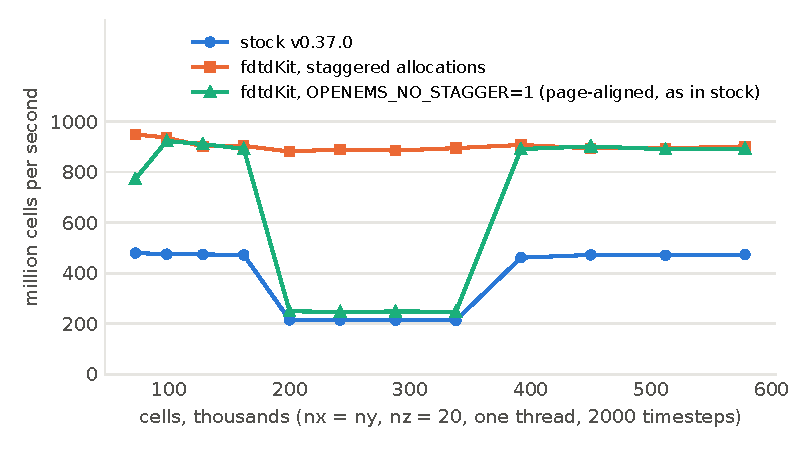
\includegraphics[width=0.7\textwidth]{fig_cache}
\caption{The allocation-placement valley on one thread: PEC box with $N_z=20$, 2\,000 steps. \mbox{fdtdKit}: the
installed cg16 build on 2026-11-01, with staggered allocations and with \code{OPENEMS\_NO\_STAGGER=1}, which leaves
the field arrays page-aligned as in stock (\code{results/cache\_valley\_2026-11-01.txt}; the low no-stagger point at
72\,000 cells is one run that was not re-measured). Stock v0.37.0: measured on 2026-11-03
(\code{results/cache\_valley\_stock\_2026-11-03.txt}).}\label{fig:cache}
\end{figure}

\subsection{PML slabs that do not span z: a scalar-SSE path and compressed tables (cg11, cg14)}
The SMA launch did not gain from the stagger. Its PML is a z-only slab at the top (13\,\% of the cells) and the UPML
vector path requires a full-z box, so those cells ran the original template: 202\,\MC\ single thread, 654 with the PML
swapped for Mur. The fork adds a scalar-SSE path for any PML box that is not a full-z slab: per local $z$ the float
offset inside an $(x,y)$ row of vectors is tabulated once ($12(z \bmod n_v) + z/n_v$), the hooks iterate rows,
components and $z$ with contiguous flux and coefficient rows, and the expression is literally the template's
($f = vv\cdot V - vv_{\text{fo}}\cdot\text{flux}$, then the swap), so the compiler contracts it the same way; each
cell-component touches only its own $V$ and flux, so the loop order does not change values. With line hooks the fused
sweep now covers the slab. SMA single thread 202 to 405, 4 threads 436 to 737, 8 threads 951 (cg29 runs this path four
y-rows at a time, Section~\ref{sec:cg29}). Of the test models only
the SMA launch, with its top z slab, takes this path. A notch tutorial run with \code{PML\_8} requested on all six
faces (\code{results/notch\_s1\_n8000\_pml6.txt}) does not: on its 14 z lines openEMS resets the z PML to PEC, and the
four x and y slabs span the whole z range. The 69\,500 distinct
operators of the SMA model cost only about 11\,\% (standalone kernel with 70\,000 operators; from the project log).
cg14 then lets the hooks read a table of distinct coefficient sets (24\,B scalar or 96\,B vector entries, a few
hundred of them: the PML profile times the materials) through a 4-B index, instead of the six per-cell coefficient
arrays (72\,B per cell). The index is per cell-component on the scalar-SSE path and per z-vector component (four
cells) on the vector path. The operator extension keeps its arrays, as in stock, and the vector path frees its own
vector copies of them, so the gain is in traffic, not in memory: with the index (and, on the vector path, the vector
copies of the flux) a PML cell holds more memory than in stock. \code{OPENEMS\_NO\_PML\_TABLE=1} keeps the hooks on
the per-cell arrays. Bandwidth-side only: SMA 4 threads 1\,137 to 1\,241, notch x3 8 threads 2\,022 to 2\,099; single
thread unchanged.

\subsection{Line hooks for the dispersive extension (cg12)}
The optimisation review of the branch found the real GCPW problem: every lossy board uses \code{AddConductingSheet},
whose engine extension (\code{Engine\_Ext\_LorentzMaterial} on \code{Engine\_Ext\_Dispersive}) implemented only the
non-threaded hooks, so the multithreaded engine ran them on thread 0 through \code{GetVolt}/\code{SetVolt}, declared
nothing (19 barriers per step on that model at cg11) and kept the whole run on the unfused plan. The fork gives the
dispersive extensions line hooks: the auxiliary-differential-equation positions of every order are stable-sorted by
x, the float index of each component is precomputed, the per-position arithmetic is the template's (apply:
$v \leftarrow v - \text{ade}$; Lorentz pre-hooks: the template's three statements), and the extension declares the
pre/apply voltage and current groups only for the orders that have such terms. Positions on different x cannot share
a cell, and positions on the same x keep their original order, so even a duplicated cell would be updated in the
stock order. Verified on the GCPW line and on a Drude/Lorentz box exercising both branches (plasma only, plasma plus
pole; template versus line hooks; raw fields; 1 and 4 threads). GCPW 4 threads 868 to 1\,435--1\,661\,\MC; cg29 runs
the two orders of a conducting sheet back to back, four positions at a time (Section~\ref{sec:cg29}). The threaded
whole-grid hooks of these extensions are still not parallelised; they matter only when something else forces the
unfused plan. The same snapshot hardened two things the correctness review flagged: the per-thread material-lookup
cache in the operator setup keys on the first and last primitive as well as the coordinate and the vector address,
and \code{SetupCSXGrid} clears the tabulated mesh deltas.

\subsection{Packed coefficient tables (cg13)}
The compressed operator keeps its coefficients in twelve structure-of-arrays tables (four coefficients $\times$ three
components, 16\,B entries); a voltage update needs six of them for one operator index, up to six cache lines, and with
the 69\,500 operators of the SMA model on its 1.071\,M-cell mesh (13.3\,MB of tables; operator count from the project
log) the access is sparse.
\code{Engine\_SSE\_Compressed::Init} copies them into two per-operator arrays of six vectors in the order the update
reads them (\code{struct PackedCoeff \{f4vector c[6];\}}, 96\,B), and the IJKN loops read those: one or two lines per
operator, +13\,MB for the SMA model. Plain copies, same floats. \code{OPENEMS\_NO\_PACKED\_COEFF=1} skips the build,
and because the IJKN loops require the packed table, that knob also reverts to the generic loops and the unfused
sweep: it is an ``old engine'' switch, not an isolated A/B.
The same happens when the tables cannot be allocated: both are freed and the engine runs the generic loops, unfused.
GCPW 1 thread 507 to 532; SMA 1\,017 to 1\,137 at 4 threads. At 4 threads the GCPW runs of cg12 to cg14
(1\,608--1\,745) lie within the run-to-run spread, so no gain is credited there. Since cg29 a model whose packed tables
would exceed 4\,MB gets smaller geometry tables instead (of the six, only the SMA launch; Section~\ref{sec:cg29}).

\subsection{Thread quality of service (cg15)}
On macOS the engine threads now run at \code{QOS\_CLASS\_USER\_INITIATED} (\code{OPENEMS\_QOS=0} off, 2 =
user-interactive, same speed), set right after the subnormal setup in each worker. Stock workers ran at the default
class, which lets the scheduler park them on E cores or behind foreground applications. Scheduling only; probes
bit-identical. Measured in a separate session (from the project log; not in \code{results/}): SMA 8 threads
1\,304--1\,385 to 1\,409, notch x3 8 threads 2\,039 to 2\,102, 10 threads 1\,657 to 1\,856; 4 threads unchanged. The
cg14 check runs in \code{results/}, without QoS, already reach 1\,385 (SMA, 8 threads) and 2\,099 / 2\,038 (notch x3,
8 / 10 threads), so the gain is within the run-to-run spread of a shared machine. The cg17 runs in \code{results/}
were made on a loaded machine and are not comparable. A per-thread split of the classes between P and E cores (second
review, item 4) was measured for cg29 and dropped; every thread keeps the user-initiated class
(Section~\ref{sec:rejected}).

\subsection{On the bit-identity argument}\label{sec:contract}
Some items rely on the compiler contracting the rewritten expression the way it contracted the stock expression:
the IJKN loop and the UPML vector rows (a rounded product plus one fused multiply-add; the y-row groups of cg29's
scalar UPML path use the vector rows' form), the Mur fast path (one fused multiply-subtract or multiply-add per update)
and cg29's merged sheet ADE (the template's statements on four lanes). This was verified by comparison with stock on
every model and, for the cg29 items, on boxes against the template hooks; the IJKN loop was also checked against the
Swift/Metal prototype, which calls \code{fma()} explicitly there and has no Mur or UPML. The Metal diamond engine
(Section~\ref{sec:gpu}) runs Mur, UPML, lumped RLC and the dispersive extensions on the GPU with \code{fma()} where
clang fuses and Metal's fast math off, and it is bit-identical to the multithreaded engine run with
\code{OPENEMS\_FTZ=1} on the six models and in the 72 comparisons of \code{scripts/checks/diamond\_check.sh} (cg28 and cg29),
so these paths now also agree with an independent implementation. The contraction is not forced in the C++ source (no
\code{fma()} calls, no \code{\#pragma STDC FP\_CONTRACT}), and it holds for clang, whose default contracts within one
expression. GCC contracts across
statements by default (\code{-ffp-contract=fast}): on aarch64, and on x86-64 when FMA is enabled, it fuses the other
product than stock in the IJKN loop and the UPML vector rows. For the inner loop the effect was measured in the
standalone kernel (\code{results/kernel\_gcc\_vs\_clang\_2026-11-03.txt}, three grids, five rounds): the stock loop
gives the same bits under Apple clang and GCC~16, and the clang-built rewrite equals it bit for bit, while the
GCC-built rewrite differs from the GCC-built stock loop on every grid and round, because the two forms then round a
different product. A GCC build of openEMS was not made, so the effect on whole runs was not measured; such a build
would be correct but not bit-identical to stock. A bit comparison under GCC needs both builds made with
\code{-ffp-contract=off} (upstream's Debug build sets it). A reader porting the fork should run \code{check.sh} once;
it is macOS-only, since it selects the libraries through \code{DYLD\_LIBRARY\_PATH}. Making the contraction explicit
in both the stock-equivalent and the new paths is a reasonable follow-up.

\subsection{What a cell costs now}
On a model larger than the cache a time step streams the six field arrays once (24\,B read, 24\,B written), reads the
operator index (1\,B per cell: one 32-bit entry per z-vector since cg29, up to 4\,B as allocated before), and takes
the coefficient tables, the PML tables and the neighbours' lines from L2: 49\,B per cell of DRAM traffic (up to cg28,
52\,B when $N_z \le 42$). The exception is a graded mesh with many distinct operators: the SMA launch on its
0.871\,M-cell mesh has 64\,410 of them and 12.4\,MB of packed tables, which stream from memory next to the fields;
cg29's geometry tables take 100 instead of 192\,B per operator (Section~\ref{sec:cg29}). On models that fit the cache
the per-step cost is the synchronisation (two barriers up to cg28, the neighbour flags since), the hooks and the
dumps, which is why the tutorials top out at about 1\,900\,\MC\ rather than higher.

\subsection{Review fixes (patches 0005 and 0006)}\label{sec:reviewfixes}
A further AI-assisted read-only correctness review of the branch (Section~\ref{sec:disclosure}), run before
publication, found one wrong-result bug; patch 0005 (snapshot cg17) fixes it and six smaller things; the four earlier
patches are unchanged. A final review led to patch 0006 (below).
\code{Engine\_Ext\_DebyeMaterial} implements the pre- and post-voltage hooks but inherited \code{GetUsedHooks()} from
\code{Engine\_Ext\_Dispersive}, which declares only the apply group and line hooks, so the hook plan never called them
and the fused sweep accepted the extension: the multithreaded engine ran a Debye cell as its base material while the
single-threaded engines, which call every hook, were right. No model of the suite has a Debye material (its dispersive
checks used Drude/Lorentz and conducting sheets), and bit identity covers only what the models exercise. The fix
declares the two hooks (no line hooks then: the fused sweep was off with Debye materials until cg29 gave them line
hooks, Section~\ref{sec:cg29}), and a structural guard,
\code{OPENEMS\_HOOKS\_DECLARED\_BY} at the top of every \code{GetUsedHooks()} override, hands a subclass that does not
override it the stock every-hook set, so a declaration cannot be inherited again. \code{scripts/checks/debye\_check.sh}
($60\times60\times20$ Debye box, 600 steps, final fields compared bit for bit): before the fix the largest voltage
difference was 37\,\% of the peak voltage and 187\,108 of 216\,000 voltage values differed; after it the fields are
bit-identical and the single-threaded result is unchanged (rerun with 2 threads during the final review; the output
is not in \code{results/}).

The smaller fixes of patch 0005: the probe end hold can start only once every probe has a non-zero peak (a far port
the pulse had not reached counted as settled). This catches only a probe that is still exactly zero. The numerical
precursor of the pulse gives a far probe tiny non-zero values some time before the pulse arrives, the longer before
the farther the probe; measured against $10^{-6}$ of the largest peak of its kind, they count as settled, so the hold
must still be longer than the longest one-way delay. The GCPW stop point is unchanged: 45\,570 steps before the fix
(cg16, from the project log) and on cg18 (row \code{G\_60} of \code{results/rfsim\_e2e\_2026-11-03.txt},
its port files a byte-identical prefix of the full run's). Further: the setup's
material-lookup cache also keys on a setup generation counter (no stale hits in a later setup of the same process);
the excitation declares the apply-current hook only when it has current excitations (one barrier per step less,
unfused); the thread tuner clamps its larger candidates to the number of x-lines; the separable nf2ff path is used
only with Apple's Accelerate (other builds keep the threaded legacy loop); the packed coefficient tables are skipped,
with a message, when they would exceed twice the field memory or fail to allocate (the size test is removed again in
patch 0006). cg17 passed a reduced check: the six models bit-identical to stock at 4, 8 and automatic threads, one run
each without the quiet wait, on a loaded machine, so the speeds in \code{results/*\_cg17.txt} are not comparable; the
cylindrical multigrid example's 18 HDF5 datasets equal; the GCPW probe end at the same step with a bit-identical
port-file prefix (these two from the project log).

Patch 0006 (snapshot cg18) holds the fixes of the final review. The packed-table size test of patch 0005 is removed
again: it could fire only through the z padding, and then it also turned off the IJKN loops and the fused sweep, so a
model with a graded material (nearly one operator per z-vector) and a z line count that is not a multiple of 4 ran on
the generic loops, unfused. The tables are always built, as in cg16; only a failed allocation skips them (both tables
freed), and the multithreaded engine then says that the fused sweep is off because there are no packed tables. The
on/off knobs act only when set to a value other than empty or \code{0}. The probe end criterion counts the excitation
as running until its signal length plus the largest excitation delay (the voltage and current entries of every grid,
including the multigrid child grids, and the TFSF propagation delay); a mode-match probe counts with its mode
amplitude only, not with its purity; a probe that has seen no signal still holds the run, but once every other probe
has settled the run prints a one-time notice naming it; an invalid \code{OPENEMS\_PROBE\_END\_DB} or
\code{OPENEMS\_PROBE\_END\_HOLD} prints a warning. The tuner clamps every candidate, including P$-$2 and the start.
With \code{OPENEMS\_FTZ} the creating thread gets its previous flush-to-zero bit back when the engine is destroyed on
it. Each level engine of a cylindrical multigrid prints its fused-sweep line once (each printed it twice before); the
per-block work buffer of the separable nf2ff path is bounded; the Accelerate include builds with GCC on macOS, and the
spin barrier's yield is guarded for 32-bit ARM; a mesh whose node count overflows the 32-bit array sizes (above
$2^{32}/3 \approx 1.43\times10^9$ nodes when arrays with three components over the whole mesh are needed, as with
field dumps or an nf2ff box; $2^{32}\approx 4.29\times10^9$ otherwise) is refused with a clear error; the raw
\code{OPENEMS\_EXPORT\_*} export reports failed writes; code comments are corrected; and the build reports its real
git revision (the cg16 and cg17 libraries both call themselves v0.37.0-19-g0893f50).

cg18 went through the full check on a quiet machine on 2026-11-03: \code{check.sh} ran the six models at
1, 4, 8 and 10 threads and with the automatic choice, two runs each, and every run was bit-identical to stock in
probes and S-parameters (\code{results/*\_cg18.txt}). The other checks of that day are in
\code{results/correctness\_cg18\_2026-11-03.txt}: the Debye box of \code{debye\_check.sh} gave the same fields in the
basic, sse-compressed and multithreaded (4 threads) engines, and the same as cg17; the cylindrical multigrid example
(1.37\,M cells, 1\,500 steps, 4 threads, one frequency- and one time-domain dump) showed 0 differences against stock
in 34 HDF5 datasets (the 18-dataset checks above used a different run length); the patch tutorial's far field was
bit-identical to cg17's and, with \code{OPENEMS\_NF2FF\_LEGACY=1}, to stock's, and the separable path stayed within
$6.8\times10^{-7}$ of stock's pattern maximum. The validation suite (Section~\ref{sec:repro}) passed 15 of 15 checks
with the multithreaded engine at 4 threads and with the default engine and thread count
(\code{results/validation\_cg18\_mt4.md}, \code{validation\_cg18\_fastest.md}). The probe-end runs of
Table~\ref{tab:probeend} were made with this build (\code{results/rfsim\_e2e\_2026-11-03.txt}); the GCPW line stops
after 45\,570 steps, as before, with a byte-identical port-file prefix.

Documented in \code{BUILD.md}, not changed: the operator setup uses every core whatever \code{numThreads} says;
\code{OPENEMS\_FTZ} has no effect on \code{--engine=basic}, which never calls the subnormal setup; with GCC's default
contraction the rewritten loops round a different product than stock, so a GCC build would not be bit-identical
(measured in the standalone kernel only, Section~\ref{sec:contract}); a run that ends on the energy
criterion can stop at a different step than v0.37.0, because the base checks that criterion on a different schedule
(upstream eb1c5ee, Section~\ref{sec:policy}), while bit identity holds for the same number of steps; upstream fixes
made after the base are not in the fork (among them 367a63f, flush to zero only during the run and
for every engine; 54a4c60, setup and run errors caught instead of terminating Python; d1fef7c, no excitation before
its delay, which matters for delayed step and custom excitations; 0212258c3, correct sizes and counts for large
meshes); the libraries are not ABI-compatible with v0.37.0 builds (the base's ArrayLib \code{m\_owner} member and the
staggered allocator), so after any install over another build both Python modules must be rebuilt for SAR (FDTD
runs and nf2ff are not affected); the bodies of the five earlier commit messages are kept as written, and the message
of 0006 lists their corrections.

\subsection{The second review's CPU items and other contributors' ideas (cg29, patches 0017--0027)}\label{sec:cg29}
Snapshot cg29 (2026-11-05; eleven commits on cg28, one per topic) holds the CPU items of the second optimisation
review (Table~\ref{tab:review2}) and the ideas of other contributors' openEMS work that the fork did not have yet
(Section~\ref{sec:positioning}); cg19--cg28 had added the Metal diamond engine without changing the CPU engines
(Section~\ref{sec:gpu}). An item was kept only when a paired interleaved A/B (\code{bench/abtest.py}: the
configurations run in turn, round after round, and the ratio is taken within each round, so a slow phase of the shared
machine hits both alike) gained clearly outside the spread of the rounds on the models it is for and cost nothing
outside the noise on the others. One exception: 0021 cost upstream's ideal case 20\,\% at 8 threads (0.80$\times$)
and was kept because the steady-state detection on the flags (0026) recovers most of it (1.18$\times$ at 8 threads).
Most A/Bs ran knob against knob in one build; 0020 and 0026, which have no knob, and
0027 were compared with the build before them, and 0021 and 0022 with \code{OPENEMS\_FUSED=0}. The ratios are medians
of the per-round ratios,
with the other processes' load in cores; the SMA launch is the 0.871\,M-cell model of the toolkit's default mesh. The
numbers are from \code{results/cpu\_items\_cg29\_2026-11-05.txt} (section 1 for the kept items, section 2 for the
dropped ones, which Section~\ref{sec:rejected} lists) unless a commit message is named. Table~\ref{tab:cg29} has the
eleven commits.

\paragraph{Operator index per z-vector (0017).} The compressed operator allocated its index with one 32-bit entry per
cell, although the operator and the engines read only the entries of the z-vectors (memory layout above); on meshes of
up to 42 z lines the engines therefore streamed 4\,B of index per cell instead of 1\,B. The index is now allocated
per z-vector: the same values in a smaller array. \code{OPENEMS\_OP\_INDEX\_PER\_CELL=1} keeps the old allocation.
Patch x5 1.119$\times$ at 4 threads and 1.101$\times$ at 8, notch x3 1.042$\times$ and 1.052$\times$, the other four
models 1.005--1.021$\times$ (5 rounds, 0.3--1.4 cores; the commit message gives 0.4--1.7);
about 3\,B per cell less memory (15.8\,MB on notch x3, 23.6\,MB on patch x5, commit message).

\paragraph{Conducting-sheet orders merged (0018; review item 2).} A conducting sheet is a two-order ADE on one set of
positions, already in x order, and the line hooks of cg12 ran each order over all positions, one float at a time.
When every order with voltage (current) terms has the same positions in x order, the pre-update
(\code{Engine\_Ext\_LorentzMaterial::PreMerged}) and the apply (\code{Engine\_Ext\_Dispersive::ApplyMerged}) now run
the orders back to back per position, four positions at a time as \code{f4vector}s, with the field values gathered and
scattered lane by lane. Every float sees the same operations in the same order: the states of different orders are
independent, and the apply still subtracts order 0 before order 1. Because the apply scatters four positions at once, a
position listed twice in one group of four would lose an update, so the merge also requires every position to appear
once (the builders list each cell once, so the guard never fails today). The guard follows the strict-order check of
upstream PR \#245 by Roel Bud\'e (unsettledroell404)~\cite{pr245}; the rest of that PR, the unfused hooks split over
the threads, is not needed, since the line hooks already run on every thread. \code{OPENEMS\_ADE\_MERGED=0} runs one
order after the other. GCPW line (6\,624 sheet positions) 1.041$\times$ at 4 threads and 1.031$\times$ at 8 (8 rounds,
0.3--0.5 cores), against the review's estimate of +8--12\,\%; no effect on the models without sheets.

\paragraph{UPML scalar path, four y-rows at a time (0019; review item 1).} The scalar-SSE path of cg11 (above) took 13
instructions per cell and component in its inner loop: a lane offset, a table index, two coefficients, the flux and the
field value. With the coefficient table of cg14, four consecutive y-rows of an x-line now form a group whose fluxes and
coefficient sets are stored per group (lane = row), so a group takes one vector operation per step of the update while
the field values are gathered and scattered lane by lane, about 7 instructions per cell. A box that is not a multiple
of four rows wide runs the last group of an x-line lane by lane on the same arrays, and the threads get whole groups.
The vector statements have the form of the UPML vector rows ($p=-(c_{\text{fo}}\cdot F)$, $f = c\cdot E + p$), the
same operations per cell as the scalar path. \code{OPENEMS\_PML\_YVEC=0} keeps the scalar rows. SMA launch
1.183$\times$ at 1 thread, 1.125$\times$ at 4 and 1.129$\times$ at 8 (6 rounds, 0.4--0.6 cores;
421 to 498, 1\,256 to 1\,403 and 1\,303 to 1\,471\,\MC\ in the commit message, which gives 0.4--0.7 cores), against
the review's estimate of +15--25\,\%.

\paragraph{UPML coefficients on the setup threads (0020; PR \#244).} The UPML operator extension computed the PML
coefficients of every cell on one thread, evaluating the grading function through the function parser for every cell
and component. From upstream PR \#244 by Noriaki Takashima (nori-proto)~\cite{pr244} the fork takes the UPML part and
its \code{RunJobsInThreads()} helper: the x-lines are split over the operator's setup threads
(\code{GetNumSetupThreads()}, so the single-threaded engines keep a one-thread setup), each thread evaluates the
grading on its own copy of the parser, which is not reentrant, and an exception in a thread is rethrown on the calling
thread. The PR's Debye part is not taken (Section~\ref{sec:rejected}). Same values in every cell; there is no knob.
UPML build time (\code{OPENEMS\_SETUP\_TIMING=1}, 6 rounds; 0.3--0.5 cores of other load, commit message): SMA launch
0.086 to 0.022\,s (operator setup 0.32 to 0.24\,s), notch x3 0.090 to 0.035\,s (1.46 to 1.38\,s), notch tutorial
0.013 to 0.005\,s.

\paragraph{Steady-state detection and Debye materials on the fused sweep (0021, 0022).} A sinusoidal excitation adds
openEMS's steady-state detection, and that extension had no line hooks, so the multithreaded engine ran every such
simulation, all cases of upstream master's \code{benchmark} tool among them, on the unfused plan. Its
\code{Apply2VoltagesLines()} now records the E-field probes of its x-lines and, on an evaluation step, copies the
voltages and currents of its lines (24\,B per cell, allocated at the first evaluation step of a fused run); the thread
that copies the last lines evaluates the period from the copies with the same energy sum. The unfused hook sees the
voltages after their update and the currents before theirs, and so do the copies, line by line, so the values, the
operations and the stop step are unchanged. The Debye extension's own pre- and post-voltage hooks get line versions
that run the same per-position operations in x order; every position has its own state and reads only its own cell.
Neither commit adds a knob; the A/B ran against \code{OPENEMS\_FUSED=0} in the same build, on upstream's cases (1\,M
cells, 3\,000 steps, 5 rounds, about half a core of other load according to the commit messages): pml 1.36$\times$ at 4
threads (at 8 within the noise), inhomogeneous 1.29$\times$ at 4 and 1.34$\times$ at 8, ideal 0.98$\times$ and
0.80$\times$ (a homogeneous box, where the unfused plan's work stealing evens out the threads within a step; the
neighbour flags below recover most of it), and the dispersive case, a Lorentz and a Debye block, 40.8 to 263.9\,\MC\ at
4 threads (6.5$\times$) and 43.8 to 439.9 at 8 (10.0$\times$), since the unfused plan ran the Debye hooks on one thread.

\paragraph{Geometry coefficient tables (0023; review item 9 in another form).} The packed tables of cg13 hold all six
coefficient vectors of an operator for each update, 192\,B per operator. A graded mesh has many distinct operators
(the SMA launch 64\,410, 12.4\,MB of packed tables), and the tables then stream from memory next to the fields. Most of
these operators differ only in their edge lengths: $vi$ ($iv$) carries the geometry, $vv$ ($ii$) the material. The
geometry layout keeps the three $vi$ ($iv$) vectors per operator, 48\,B in operator order, and a 16-bit index into a
small table of the distinct $vv$ ($ii$) triplets: 100\,B per operator for both updates. The IJKN loops take the six
coefficients from either layout, the same values into the same operations. The geometry layout is chosen when the
packed tables would exceed 4\,MB, and the packed one when there are more than 65\,535 distinct triplets;
\code{OPENEMS\_COEF=packed} or \code{geom} forces one, and the fused sweep runs on either. SMA launch 1.067$\times$
[1.021--1.116] at 8 threads, 1.033$\times$ with the automatic count, 1.025$\times$ at 4 (noisy) and 0.992$\times$ at 1
(8 rounds, 0.3--0.4 cores). The other five models have at most 1.5\,MB of packed tables and stay packed (geometry
tables lose 2--5\,\% there at 4 threads, commit message). The review's form of the item, the distinct vectors in one
table and four 16-bit ids per operator, gave nothing on the four models measured (0.933--1.023$\times$;
Section~\ref{sec:rejected}).

\paragraph{Neighbour flags (0024, 0025; review item 5).} \code{OPENEMS\_FUSED\_STAT=1} (0024, a diagnostic) times
every thread of the fused sweep: at 8 threads the threads waited 24--27\,\% of the time at the two barriers. A thread
needs only its neighbours: the voltages of its last x-line need the currents of the line after its slab, which the
next thread updates as its line before the slab, and its line before the slab needs the final voltages of the previous
thread's last line. \code{FusedTimestepFlags()} (0025) replaces the two barriers by two step counters per thread; a
wait spins like the spin barrier and then sleeps on a condition variable, with sequentially consistent stores and loads
so that no wake-up is lost. Before its last block a thread waits until the next thread has done its line before the
slab in the previous step, then publishes its sweep; before its line before the slab it waits for the previous
thread's sweep of this step, then publishes that line. Every cell sees the same operands as with the barriers.
Neighbours are then at most one step apart, threads $t$ and $t+k$ at most $k$, so the extensions' line hooks must not
depend on a common step: an extension declares \code{TS\_LOCAL} when its line hooks keep no state shared by x-lines
that changes from one step to the next and read the step through \code{GetNumberOfTimesteps()}, which returns the
calling thread's own count while the flags run. Mur, UPML, the excitation, the dispersive family (Drude/Lorentz,
conducting sheets, Debye) and the lumped RLC declare it. The lumped RLC used to move its $[n]$, $[n-1]$, $[n-2]$
containers on by a pointer rotation once per step, done by the first thread to arrive; it now takes them from the step
number (slot $k$ at step $n$ is array $(k-n-1) \bmod 3$), the same arrays as the rotation: a slot indexed by the time
step, as MrHighVoltage proposed in upstream Discussion \#492~\cite{mrhv492}. With an extension that does not declare
\code{TS\_LOCAL} the barriers stay and a verbose message names it; \code{OPENEMS\_FLAGS=0} keeps them too. A stress run
in which every wait that is not satisfied at once sleeps (\code{OPENEMS\_BARRIER\_SPIN\_US=0}, at 3, 8 and 10 threads
and the automatic count, under a watchdog) did not hang. Flags against barriers (5 rounds, 0.3--0.6 cores):
1.015--1.055$\times$ at 4 threads and 1.073--1.286$\times$ at 8 on the six models (Table~\ref{tab:cg29}); with them
the threads wait 10--22\,\% of the time at 8 threads (patch x5, SMA, GCPW; commit message). The review had estimated
0--3\,\% on the GCPW line, +3--8\,\% on the SMA launch and +4--10\,\% on the large models at 8 threads; the GCPW line
gained most, 1\,337 to 1\,719\,\MC\ (1.286$\times$).

\paragraph{The steady-state detection on the flags (0026).} The detection kept the barriers: it recorded its probes in a
ring of two periods, and the evaluation of a period assumed every thread at the same step. With the flags a thread can
be up to the thread count of steps ahead of another, so the ring now keeps three periods (the record of step $n$ at
$n \bmod 3p$ for a period of $p$ steps), and an evaluation reads the last two periods by step. While a period is
longer than twice the thread count, no thread reaches the next evaluation step or overwrites a record of the last two
periods before the evaluation of this one is done, and the extension then declares \code{TS\_LOCAL}. Same records, same
sums in the same order. No knob of its own; against the build before (5 rounds): upstream's ideal case (1\,M cells,
3\,000 steps) 1.18$\times$ at 8 threads and 1.13$\times$ with the automatic count, ideal M (8\,M cells, 600 steps)
1.07$\times$ and 1.05$\times$, inhomogeneous 1.41$\times$ and pml 1.05$\times$ at 8 threads (these two under 1.5--3
cores of other load, commit message).

\paragraph{No flag spin above the P-core count (0027; review item 4 in part).} With more threads than performance
cores some threads run on the efficiency cores, the waits for them are long, and a spinning thread takes power and a
core from the others. The flag waits now spin for the barriers' spin time only up to the P-core count
(\code{hw.perflevel0.physicalcpu}); above it a wait makes its first 128 checks and then sleeps, while the barriers
keep their spin at every thread count. On other CPUs the
barrier spin time is kept (not measured there). \code{OPENEMS\_FLAGS\_SPIN\_US} sets the spin for any thread count.
Scheduling only. Against the build before (4 rounds, 0.3--0.5 cores): GCPW line 1.088$\times$ [1.086--1.133] at 8
threads and 1.123$\times$ with the automatic count, notch tutorial 1.094$\times$ and 1.051$\times$, 4 threads unchanged
(0.999$\times$, 0.998$\times$). Sleeping at once also at 4 threads, all on P cores, cost notch x3 2\,\% in every
round, so the spin stays there.

\paragraph{Identity.} The checks of cg29 ran on 2026-11-05 from 02:01 to 02:41 (section 3 of the results file).
\code{check.sh} ran stock as the reference, at its thread count per model (8 threads for patch x5 and notch x3, 2 for
the patch tutorial, 4 for the notch tutorial and the two boards), against cg29 at 1, 4, 8 and 10 threads, the
automatic count,
the geometry tables forced at 4 threads, the packed tables forced at 8 and the barriers instead of the flags at 8:
every run of the eight cg29 configurations equals the reference on all six models in probes and $S$-parameters
(\code{results/*\_cg29.txt}; their speeds are the faster of two unpaired runs under the check's load, not
comparisons). The Debye box of
\code{debye\_check.sh} gives the same fields in the basic, sse-compressed and multithreaded engines, and the same as
cg28. The validation suite passed 15 of 15 checks with the multithreaded engine at 4 threads and with the fastest
engine (\code{results/validation\_cg29\_mt4.md}, \code{validation\_cg29\_fastest.md}); the Metal diamond engine had
passed it at cg23 and cg27 (\code{validation\_cg23\_metal.md}, \code{validation\_cg27\_metal.md}). The cylindrical
multigrid example showed 0 differences against stock in 34 datasets. Boxes against the template hooks of the same
build: conducting sheets and Drude/Lorentz 16 of 16 identical, UPML 25 of 25, Mur 35 of 35, the steady-state detection
42 comparisons and 49 more on the flags. A run-mode matrix of 45 small models in 11 modes against stock's basic engine
(its multithreaded engine at 1 thread on cylindrical meshes): cg29's basic, sse and sse-compressed engines, its
multithreaded engine at 1, 2, 4 and 8 threads, with the barriers, unfused and with the geometry tables, and stock's
multithreaded engine at 2 threads. It gave 461 identical comparisons; the other 10 are one model on the energy end
criterion, which every cg29 mode stops at step 255 while stock runs to its limit of 1\,496 steps, with the 64 probe
lines up to the stop equal to stock's. The cause is the base, which checks that criterion earlier in short runs
(upstream eb1c5ee, Section~\ref{sec:policy}), not cg29. \code{diamond\_check.sh} gave 72 of 72, and the Metal diamond
engine equals the multithreaded engine run with \code{OPENEMS\_FTZ=1} on the six models (\code{results/*\_cg29gpu.txt}).

\paragraph{Against cg18.} Paired against cg18 (5 rounds, 0.3--0.6 cores, each model on its default mesh; notch x3 at
the automatic count from four quiet rounds measured afterwards; section 4 of the results file), cg29 runs
1.03--1.23$\times$ at 4 threads, 1.13--1.44$\times$ at 8 and 1.13--1.42$\times$ with the automatic count; the largest
gains are at 8 threads on the two boards and the notch tutorial (1.39--1.44$\times$), where the flags count most. On
the 1.071\,M-cell mesh of Table~\ref{tab:current} the SMA launch gains 1.37$\times$ at 8 threads and 1.38$\times$ with
the automatic count (4 rounds, 0.6--0.7 cores). On upstream's benchmark cases, which cg18 runs on the unfused plan
(paired, 4 rounds that waited for a quiet Mac, the other processes on a median of 0.4--1.4 cores; every run identical
across the builds; section 5 of the results file), cg29 runs 1.11--1.36$\times$ as fast as cg18 on the homogeneous
ideal box, 1.74--2.18$\times$ on the pml and inhomogeneous cases and 4.25--7.40$\times$ on the dispersive case (the
ideal box of 8\,M cells at 8 threads and with the automatic count ran under load and is left out of these ranges).
The absolute rates move between sessions, so the paired ratio is the comparison; Table~\ref{tab:current} has stock,
cg29 and the Metal diamond engine side by side.

\begin{table}[htbp]\centering\small
\setlength{\tabcolsep}{4pt}
\begin{tabular}{@{}l>{\raggedright\arraybackslash}p{0.40\textwidth}>{\raggedright\arraybackslash}p{0.45\textwidth}@{}}
\toprule
patch & change \newline knob & paired A/B, median ratio; rounds (others' load, cores) \\
\midrule
0017 & operator index per z-vector, not per cell \newline \code{OPENEMS\_OP\_INDEX\_PER\_CELL=1}: old &
  patch x5 1.119$\times$ (4 thr), 1.101$\times$ (8); notch x3 1.042$\times$, 1.052$\times$; the other four
  1.005--1.021$\times$; 5 (0.3--1.4) \\
0018 & sheet ADE orders back to back, four positions per \code{f4vector} (item 2) \newline
  \code{OPENEMS\_ADE\_MERGED=0}: old & GCPW 1.041$\times$ (4 thr), 1.031$\times$ (8); models without sheets
  unaffected; 8 (0.3--0.5) \\
0019 & UPML scalar-SSE path, four y-rows per group (item 1) \newline \code{OPENEMS\_PML\_YVEC=0}: old &
  SMA 1.183$\times$ (1 thr), 1.125$\times$ (4), 1.129$\times$ (8); 6 (0.4--0.6) \\
0020 & UPML operator coefficients on the setup threads (PR \#244) \newline no knob &
  UPML build SMA 0.086 to 0.022\,s, notch x3 0.090 to 0.035\,s, notch tutorial 0.013 to 0.005\,s;
  6 (0.3--0.5)$^a$ \\
0021 & steady-state detection: line hooks \newline no knob (against \code{OPENEMS\_FUSED=0}) &
  upstream cases: pml 1.36$\times$ (4 thr), inhomogeneous 1.29$\times$ (4), 1.34$\times$ (8), ideal 0.98$\times$
  (4), 0.80$\times$ (8); 5 (about 0.5)$^a$ \\
0022 & Debye material: line hooks \newline no knob (against \code{OPENEMS\_FUSED=0}) &
  upstream dispersive case 40.8 to 263.9\,\MC\ (4 thr, 6.5$\times$), 43.8 to 439.9 (8 thr, 10.0$\times$);
  5 (about 0.5)$^a$ \\
0023 & geometry coefficient tables, 100 instead of 192\,B per operator, when the packed ones exceed 4\,MB
  (item 9) \newline \code{OPENEMS\_COEF=packed} or \code{geom} &
  SMA 1.067$\times$ (8 thr), 1.033$\times$ (auto), 1.025$\times$ (4), 0.992$\times$ (1); the other five stay
  packed; 8 (0.3--0.4) \\
0024 & per-thread time split of the fused sweep \newline \code{OPENEMS\_FUSED\_STAT=1}: on &
  diagnostic: at 8 thr 24--27\,\% of the time waiting at the barriers \\
0025 & neighbour flags instead of the two barriers; RLC slots by time step (item 5; Discussion \#492) \newline
  \code{OPENEMS\_FLAGS=0}: barriers & six models 1.015--1.055$\times$ (4 thr), 1.073--1.286$\times$ (8; GCPW
  1.286$\times$, SMA 1.109$\times$); 5 (0.3--0.6) \\
0026 & steady-state detection declares \code{TS\_LOCAL} (runs on the flags) \newline no knob of its own &
  upstream ideal 1.18$\times$ (8 thr), 1.13$\times$ (auto); ideal M 1.07$\times$, 1.05$\times$; inhomogeneous
  1.41$\times$ and pml 1.05$\times$ (8); 5 (1.5--3 for the last two)$^a$ \\
0027 & no flag spin above the P-core count (item 4 in part) \newline \code{OPENEMS\_FLAGS\_SPIN\_US} &
  GCPW 1.088$\times$ (8 thr), 1.123$\times$ (auto); notch tutorial 1.094$\times$, 1.051$\times$; 4 thr
  0.999$\times$, 0.998$\times$; 4 (0.3--0.5) \\
\bottomrule
\end{tabular}
\caption{The CPU items of snapshot cg29 (patches 0017--0027, one commit each), all bit-identical to stock v0.37.0.
Paired interleaved A/B (\code{bench/abtest.py}), median of the per-round ratios, number of rounds and the other
processes' load in cores; knob against knob in one build, 0020, 0026 and 0027 against the build before, 0021 and 0022
against \code{OPENEMS\_FUSED=0}. The SMA launch on its 0.871\,M-cell mesh. From
\code{results/cpu\_items\_cg29\_2026-11-05.txt}, section 1; $^a$~load from the commit message. Item numbers are
those of Table~\ref{tab:review2}.}\label{tab:cg29}
\end{table}

\section{Setup, post-processing, and the ceiling}\label{sec:beyond}

\subsection{Operator setup}
Creating the operator took 4.1\,s for both large models, longer than many short runs (this and the other setup times
here are from the project log; not in \code{results/}). Upstream already spreads the material averaging
(\code{Calc\_EC}, which asks CSXCAD for the material at several positions around every cell) over the multithreaded
operator's thread pool. The time-step search (\code{CalcTimestep\_Var3}, a sweep over every cell) and the coefficient
loop (\code{Calc\_ECOperatorPos}, which turns each cell's equivalent-circuit values into its update coefficients) ran
on one thread through the shared address helper. Both are now split over \code{std::thread}s with direct index
arithmetic, and the multithreaded operator's setup pool uses every core whatever thread count the engine is given
(stock sized it by the requested count). Each lookup in the averaging also got cheaper: the primitive list is passed by
const reference instead of being copied per call, and the material lookup remembers its last result per thread,
because the averaging asks for two material types at the same coordinate in a row (permittivity and electric
conductivity, then permeability and magnetic conductivity). The discretisation deltas are tabulated once; the
excitation extension skips y-z lines that contain no excitation primitive. In CSXCAD a new
\code{FindPropertyByCoordPriority} takes the primitive list by const reference and the by-value
\code{GetPropertyByCoordPriority} forwards to it (keeping the ABI); \code{CSPropMaterial::GetWeight} returns the plain
value when no weighting function is set instead of building a parameter set. Result: patch x5 4.1\,s to 0.9\,s, notch
x3 4.1\,s to 1.3\,s, with 4 engine threads (the fork's setup pool on all ten cores, stock's on four); the real boards
set up in 0.1\,s. \code{OPENEMS\_SETUP\_TIMING} (set to anything but empty or 0) prints the phase times. What remains
is flat: material averaging over box primitives. The Metal engine of Section~\ref{sec:gpu} set up its operator on one
thread until cg24 (notch x3 5.55\,s, against 2.74\,s since and 2.61\,s for the multithreaded engine; loaded Mac,
\code{results/diamond\_engine\_cg24\_cg27\_2026-11-04.txt}); it now uses the multithreaded engine's setup.

\subsection{Far field (nf2ff)}
The near-to-far-field transform summed, for every observation direction, over every face cell with its own
complex exponential: 17.9\,s for a $91\times181$ pattern at two frequencies on the patch x5 box (the nf2ff figures
are also from the project log, except those of cg18 below). On a Cartesian plane the phase factor
$\exp(jk\,\hat r\cdot\vec r)$ separates per mesh line, so the plane integral for all directions is a complex matrix
product (one \code{cgemm} per block of directions) followed by a row dot product. The separable path needs a CBLAS,
and only Apple's Accelerate is wired in: other builds, cylindrical meshes and \code{OPENEMS\_NF2FF\_LEGACY} (set to
anything but empty or 0) keep the original threaded loop. 17.9\,s to 1.0\,s (tutorial: 1.36\,s to 0.33\,s), with the
pattern within $7\times10^{-7}$ of its maximum (a weak cross-polar component can differ by more relative to its own
peak); the loop itself is unchanged and bit-identical. Measured again with cg18 (patches 0001--0006) on the tutorial's pattern
($91\times181$ directions, two frequencies): 1.21\,s with stock, 0.30\,s with the separable path, which stays within
$6.8\times10^{-7}$ of the maximum, while the legacy loop gives stock's pattern bit for bit
(\code{results/correctness\_cg18\_2026-11-03.txt}).

\subsection{Dumps and probes}\label{sec:dumps}
Field dumps and probes read the engine's fields through an interface that, for the SSE engines, located every value
with per-cell division and modulo. Upstream's GPU branch, at the commit this fork is based on (7bb294f), had
introduced a precomputed \emph{gather} (entry indices of the values a dump needs); \code{Field\_Gather\_SSE} maps those
entries to \code{f4vector} float offsets so the SSE engines use it too. The gather that upstream later merged into
master is region-based and stores nothing per node, so this mapping would have to be redone there. The patch
tutorial, whose nf2ff box is 12 time-domain dumps on a 0.1-million-cell model, went from 1\,076\,\MC\ (project log) to
1\,519\,\MC\ at 4 threads with the gather (snapshot cg2); after the Mur line hooks it ran at 1\,806\,\MC\ (cg8), and the
dumps still cost about 14\,\% there (2\,100\,\MC\ without them; project log): the CPU engines evaluate the dumps on the
main thread, and only the writing runs in the background. Upstream's asynchronous HDF5 writer is used as is; with it
the fork's base alone runs this model 1.13$\times$ faster than stock (308.5 against 273.4\,\MC, 2 threads), and with
the dumps off the two are equal (\code{results/patch\_s1\_n10500\_base.txt}, Section~\ref{sec:results}). Our own
background writer from the first snapshots was dropped as redundant. The Metal engine of Section~\ref{sec:gpu} also
leaves probes and dumps to the CPU, between its command buffers and on the shared memory; on this model its GPU was
busy 78\,\% of the time-stepping loop (cg24, \code{results/diamond\_engine\_cg24\_cg27\_2026-11-04.txt}, section 6).

\subsection{Where the ceiling is, and the GPU engines}\label{sec:ceiling}
Figure~\ref{fig:bandwidth} puts the engines measured up to snapshot cg14 on one axis: effective DRAM traffic, the
product of the speed and the bytes a cell update moves in the traffic model of Section~\ref{sec:fused}. An engine that
keeps a tile's fields on chip for several time steps has no such figure, so the diamond-blocked Metal engine of
Section~\ref{sec:gpu} is not a bar there. The traffic is
modelled, not measured with hardware counters, and the model counts the operator index as 1\,B per cell; the engine
allocated 4\,B of index per cell up to cg28 (one entry per z-vector since cg29, Section~\ref{sec:cg29}) and on meshes
with few z lines streamed all of it, so the CPU figures below are lower bounds (the whiskers in the figure show the
full 4\,B). On the $201^3$ box three independent implementations ended
within 10\,\% of each other in cell rate (1\,562--1\,670\,\MC, project log): the two unfused Metal kernels at
121--124\,GB/s of an assumed 74\,B/cell and the fused CPU sweep of the time (snapshot cg9) at 77\,GB/s of 49\,B/cell.
With the standalone material-table kernel of Section~\ref{sec:background}, the GPU kernels drew 121--127\,GB/s.
The CPU engine of cg18 was not run on that box. On another $201^3$ box, with Mur faces, the build of snapshot cg19
(cg18's CPU code and the Metal engine of Section~\ref{sec:gpu}) ran 1\,579\,\MC\ on the multithreaded engine at 8
threads, 1\,446 on the base's GPU engine and 2\,775 on the diamond engine at $K=4$ (rough, load average 2--7;
\code{results/diamond\_engine\_cg19\_2026-11-04.txt}).
\begin{itemize}
\item \textbf{Upstream's Metal engine} (\code{--engine=gpu}) as it was on the pre-merge \code{gpu-engine} branch at
  commit 7bb294f (2026-10-12): added by Sean Mollet (commit bf30fa4, 2026-10-08), with follow-up work by Thorsten
  Liebig. Upstream merged a reworked version into master as c3a956b on 2026-10-17 and has since deleted the branch;
  the merged engine was measured on 2026-11-04 (next item). 1\,638\,\MC\ on the $201^3$ box (project log); in \code{results/}
  923--1\,115\,\MC\ on the patch tutorial and 1\,622 on the notch tutorial, 1\,502--1\,519 and 1\,354--1\,358 on the
  two large models, 1\,337 (GCPW) and 1\,135 (SMA launch, 1.071\,M cells) on the real boards. Its voltage and current
  updates are separate passes. It was ahead of earlier CPU snapshots on some small models, where the CPU engine still paid more for
  per-step synchronisation, and on the $201^3$ box (against cg9); against the CPU engine of Table~\ref{tab:final}
  (cg14) and against cg18 (\code{results/*\_cg18.txt}) it is slower on all six benchmark models, and on the $201^3$
  Mur box above as well.
\item \textbf{Upstream master's merged Metal engine} (c3a956b~\cite{mollet235}, in a build of master 5fecbb5),
  measured on 2026-11-04 next to cg18 (best of two runs on a loaded Mac; \code{results/others\_2026-11-04/README.md}):
  level with cg18 on patch x5 (1\,529 against 1\,510\,\MC) and on the SMA launch at 0.871\,M cells (1\,084 against
  1\,019), slower on the other four (notch x3 1\,334 against 2\,010, patch tutorial 782 against 1\,856, notch tutorial
  1\,635 against 1\,822, GCPW line 1\,343 against 1\,634): 0.42--1.06 times cg18. The GPU engines of master and of
  luikore's pull request differ from stock by $1.7\times10^{-7}$ to $1.3\times10^{-6}$ relative in the port probes
  (float rounding; on the SMA launch master differs by $1.5\times10^{-4}$, a change in its CPU engine since v0.37.0
  that its GPU engine shows too; Section~\ref{sec:policy}). The merged engine's structure was not examined here, and
  \code{results/} has no run of it next to the diamond engine. On the PEC variant of the notch tutorial
  (Section~\ref{sec:positioning}) it ran at 2\,374\,\MC\ against cg18's 2\,053, the faster of two runs (the other
  1\,452), above the roughly
  2\,000\,\MC\ that 74\,B per cell allow from the M5's memory (Section~\ref{sec:background}); whether its kernels fuse
  the two half steps or this 0.270\,M-cell model stays in the GPU's caches was not examined.
\item \textbf{A Swift/Metal kernel} written for this project (\code{swift\_engine/}; its unblocked numbers are from the
  project log): the fork exports the compressed operator (\code{OPENEMS\_EXPORT\_OPERATOR=dir}: per-vector index, the four
  coefficient tables, the voltage excitation entries and signal) and the final fields
  (\code{OPENEMS\_EXPORT\_FIELDS=dir}); the kernel mirrors \code{Engine\_sse}'s operation order, uses \code{fma()}
  exactly where clang fuses on arm64, and runs with Metal's fast math off. It is bit-identical to every CPU engine on
  a $41^3$ box over 600 steps, and on $121^3$ to the SSE-family engines once both sides flush subnormals (see below;
  the basic engine has no flush-to-zero switch). 1\,670\,\MC\ at $201^3$, independent of the command-buffer batch size
  from 20 to 400 steps. Like upstream's engine it updates voltages and currents in separate passes. On 2026-11-04 it
  got a diamond-blocked mode (\code{--diamond K}), the prototype of Section~\ref{sec:gpu}: identical to its unblocked
  kernel and to the CPU engine of cg18 (with \code{OPENEMS\_FTZ=1} on the larger boxes) for every $K$ tried on $41^3$,
  $121^3$ and $201^3$ boxes, and 2\,445.7\,\MC\ at $K=4$ on $201^3$ (2\,574.8 at its best tile and threadgroup size)
  against 1\,540.0 unblocked (one run each, load average 6--12; \code{results/diamond\_swift\_2026-11-04.txt}).
\item \textbf{The CPU engine (cg14, cg18)}: 1\,764 and 2\,099\,\MC\ on the two large models (cg14,
  Table~\ref{tab:final}; cg18 1\,716 and 2\,046, \code{results/*\_cg18.txt}), 86--103\,GB/s at the model's
  49 bytes per cell (92--109 with the full 4-B index); a standalone fused kernel of the patch x5 shape, with a compact
  index of 1\,B per cell, tops out at 1\,932\,\MC\ on 4 threads, and one independent sub-grid per thread (no neighbour
  exchange at all) at 2\,273 on 6, 111\,GB/s at 49\,B per cell (both from the project log): that is the ceiling the
  cores see. Snapshot cg29 (Section~\ref{sec:cg29}) allocates the operator index per z-vector, as the model counts
  it, and with its other CPU items runs notch x3 1.134$\times$ [1.018--1.140] and patch x5 1.257$\times$
  [1.232--1.269] faster than cg18 at 8 threads (paired, 5 rounds, others 0.6 cores;
  \code{results/cpu\_items\_cg29\_2026-11-05.txt}, section 4); its rates are in Table~\ref{tab:current}, where its
  fastest CPU rate, notch x3 at 8 threads, is 2\,177\,\MC, below that ceiling.
\end{itemize}
The unfused GPU engines measured here (the base's and the Swift/Metal kernel) are therefore at best about as fast as
the fused CPU sweep on this machine, and upstream master's merged engine is level with cg18 on two of the six models
and slower on four. At the 121--127\,GB/s the GPU kernels drew, 49\,B per
cell would bound a fused GPU sweep at about 2\,470--2\,590\,\MC\ (computed from the traffic model; a bound, not a
prediction): 1.2--1.5 times the CPU engine of cg14 on the large models and about 1.1 times the cores' 2\,273\,\MC.
Until 2026-11-04 this section said that such a sweep was not tried and that it would need a grid-wide
synchronisation between the voltage and the current update, or halo-tiled threadgroups. The diamond engine of
Section~\ref{sec:gpu} needs neither: a tile updates its voltages and then its currents with a threadgroup barrier
between them, and four dispatches per block of steps (mountain and valley tiles in x and y) complete the tile edges.
Run with one time step per block ($K=1$) it is a fused, unblocked GPU sweep, and it reached 1\,716--1\,733\,\MC\ on
notch x3 and up to 1\,844 on patch x5 (cg27; paired, 4 rounds, others' CPU 2.5--4 cores;
\code{results/fused\_sweep\_k1\_2026-11-04.txt}), 67--75\,\% of the bound or 85--90\,GB/s at 49\,B per cell: the four
dispatches, the tile edges and the barrier between the half steps cost more than the bytes they save. Blocking over
time steps passes the bound where fusing alone does not. With $K=2$ the two models ran at 2\,123 and 2\,408\,\MC,
still below it; with $K=4$ at 2\,986 and 2\,817, above its upper end; and with the tiling chosen at run time (cg28)
notch x3 reached 3\,226\,\MC\ on a quiet Mac (Table~\ref{tab:gpuspeed}). A one-dispatch fused kernel was not built; it
would need a second copy of both fields. fp16 field storage was not tried (the half-precision normal range ends at
$6\times10^{-5}$ while late-run currents are $10^{-6}$\,A, project log, so fields need scaling; and it is not
bit-identical by construction). On the CPU, two time steps per sweep gained 10--14\,\% in the standalone kernel of
2026-10-28 (project log), on top of a fused sweep that already reuses the fields between the two half steps. An upper
bound measured for cg29 on the fork's fused loops, with one independent sub-grid per thread and so without halos or
extension hooks, gave at most 6\,\% for 2 to 4 steps (\code{results/cpu\_items\_cg29\_2026-11-05.txt}, section 2), and a
real version was not built; deeper wavefront or diamond blocking~\cite{malas2015,fukaya2018} was not tried on the
CPU. On the GPU, luikore's Metal engine~\cite{luikore228} advances a diamond of four time steps per block and reports
1.3--4.2$\times$ its own unfused path on an M4 Pro and an M5 Max, on a uniform grid without conducting sheets
(Section~\ref{sec:positioning}). It was built and run on this M5 on 2026-11-04 (\code{results/others\_2026-11-04/},
best of two runs on a loaded Mac). Its diamond path refused all six models before stepping (it names the Mur
extension, on the GCPW line the conducting sheets). On variants of five of them with every Mur face replaced by PEC,
which are speed-only cases, it ran at 0.39 to 2.00 times cg18, and its legacy path was slower than cg18 on every
model. The diamond engine of Section~\ref{sec:gpu} was not run on those variants, so the two diamond engines have not
been compared head to head.

\begin{figure}[htbp]\centering
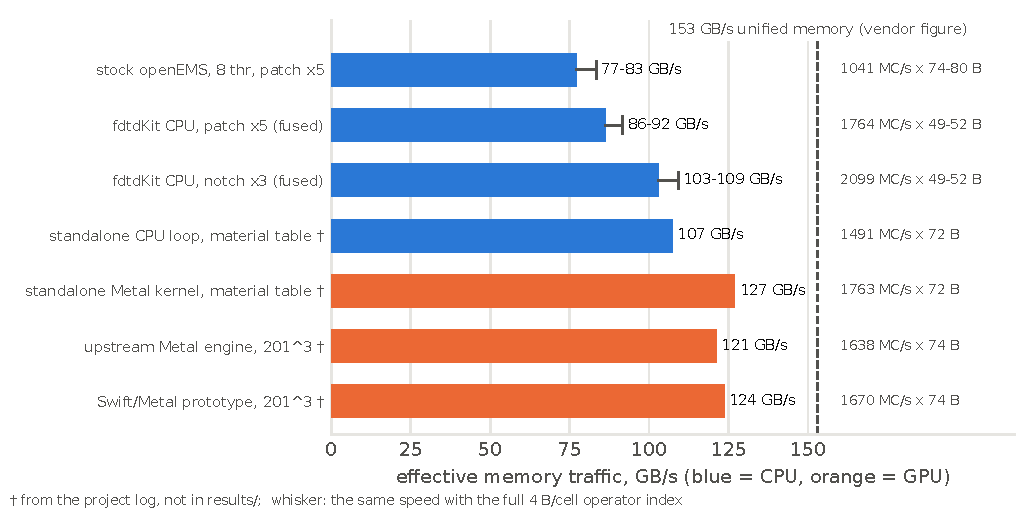
\includegraphics[width=0.9\textwidth]{fig_bandwidth}
\caption{Effective memory traffic of the engines measured up to snapshot cg14, against the M5's bus: cell rate times the bytes per cell
of the traffic model (not counter-measured). The openEMS CPU bars count the operator index as 1\,B per cell, their
whiskers the full 4\,B per cell it was allocated with up to cg28. CPU in blue, GPU in orange (upstream's pre-merge Metal engine and
the Swift/Metal prototype: assumed 74\,B/cell). The two standalone material-table kernels and the two $201^3$ bars are
from the project log, the others from \code{results/}. The Metal diamond engine of Section~\ref{sec:gpu} has no bar:
with $K$ time steps per tile its traffic depends on what the caches hold, and the traffic model gives no bytes-per-cell
figure for it (its $K=1$ case, a fused sweep, would be a bar at 85--90\,GB/s, \code{results/fused\_sweep\_k1\_2026-11-04.txt}).
Upstream master's merged engine and luikore's engine, measured on 2026-11-04, are not in the figure either.}
\label{fig:bandwidth}
\end{figure}

\paragraph{Subnormals.} The Swift/Metal kernel's first differences from the CPU engines appeared as $3\times10^{-43}$
versus 0 at step $\sim$50 and grew to $3\times10^{-7}$ of the field maximum by step 600 on the $121^3$ box (project log):
Apple's GPU flushes subnormal floats to zero, the cores keep them. Upstream openEMS sets flush-to-zero by default, but
only on x86 (a TODO in \code{tools/denormal.h} asks whether other CPUs need it). Apple's cores pay no penalty for
subnormals (the GCPW line runs at the same speed either way, \code{results/kgcpw\_s1\_n8000\_kirchftz.txt}), so the
fork keeps them by default. \code{OPENEMS\_FTZ} (set to anything but empty or 0; arm64 only) sets \code{FPCR.FZ}
in the threads of the SSE-family engines (\code{sse}, \code{sse-compressed}, \code{multithreaded}; not \code{basic})
and gives the creating thread its previous flush-to-zero bit back when the engine is torn down; with it these engines
and the Swift/Metal kernel agree on every value, and on the notch tutorial the multithreaded and sse-compressed
engines' port probes and $S_{11}$ equal those of upstream's GPU engine over 3\,000 steps (without the flush the
probes differ by $3.2\times10^{-7}$ relative; \code{results/notch\_s1\_n3000\_ftzgpu.txt}, Section~\ref{sec:policy}).
On 2026-11-04 the same held on all six models, for the base's GPU engine and for the diamond engine of
Section~\ref{sec:gpu} (\code{results/*\_cg22gpu.txt}); the diamond engine's field dumps compare equal only when both
runs set the switch, because openEMS computes them on the creating thread, which the switch also flushes
(\code{results/diamond\_engine\_cg20\_2026-11-04.txt}). A run with the flush is not bit-identical to the default run:
only subnormal values are flushed, but the difference spreads, to the
same $3\times10^{-7}$ of the field maximum after 600 steps; on the GCPW line it moved the port probes by
$4.1\times10^{-7}$ relative and $S_{21}$ by $1.8\times10^{-6}$\,dB over 8\,000 steps on one thread
(\code{results/kgcpw\_s1\_n8000\_kirchftz.txt}).

\section{A diamond-blocked Metal engine}\label{sec:gpu}
Section~\ref{sec:ceiling} ends at the memory bus. The fused CPU sweep and the unfused GPU engine of the fork's base
stream every field array from DRAM at least once per time step, and at the 121--127\,GB/s the GPU kernels drew, a fused GPU sweep that
moves 49\,B per cell is bound to about 2\,470--2\,590\,\MC. Temporal blocking moves that bound: a tile of the grid is advanced by $K$
time steps while its fields stay in the GPU's caches, so a field value need not cross the bus at every step. The
fork's engine for this, \code{--engine=metal-diamond}, was written on 2026-11-04 in ten snapshots, cg19 to cg28
(patches 0007--0016, commits 6b23756 to 68c1c82; \code{CHANGELOG.md}). Its tile schedule follows luikore's Metal
engine, openEMS PR~\#228~\cite{luikore228} (GPL; the diamond tile schedule; no code of it is used). The kernels are
the fork's own. They began as a \code{--diamond K} mode of the Swift/Metal prototype of Section~\ref{sec:ceiling},
which matched the CPU engine bit for bit at every $K$ tried (\code{results/diamond\_swift\_2026-11-04.txt}), and were
then moved onto the engine's own arrays and given the extensions that the six models use. The engine is opt-in and
Apple-only: it is built with the base's Metal option (\code{ENABLE\_METAL}), and the default engine stays the
multithreaded CPU engine. The code is \code{FDTD/engine\_metal\_diamond.h} and
\code{FDTD/metal/engine\_metal\_diamond.mm}; against cg18 the ten patches change 19 files, $+1\,717/-1$ lines, of which
the Objective-C++ file has 1\,592 (\code{git diff --stat cb168f7 68c1c82} in the fork). Snapshot cg29 leaves these
files unchanged; its CPU changes were checked against the engine (below). The build of 2026-11-11, cg31 (patches
0028--0039, of which 0029--0038 are the engine's), changes the engine again: this section describes and measures it
as of cg29, and Section~\ref{sec:cg31} has what changed and the rates since.

\subsection{Design}
\paragraph{Fields in shared memory.} \code{Engine\_Metal\_Diamond} is a subclass of the sse-compressed engine, and its
operator is, since cg24, the multithreaded engine's (\code{Operator\_Multithread}). The voltage and current arrays are
the engine's own \code{f4vector} arrays, placed in shared Metal buffers in the unified memory
(\code{ArrayENG::InitView}), so the probes, the dumps and the CPU fallback read and write the memory the kernels use,
without copies. Their order is N-I-J-K, the component outermost, instead of the CPU engines' I-J-K-N, where the three
components of a cell lie side by side and the loads of a SIMD group are 48\,B apart: on Mur boxes of $121^3$ and
$201^3$ cells N-I-J-K ran 7--9\,\% faster (GPU time, three alternating runs each, on a quieter Mac;
\code{results/diamond\_engine\_cg19\_2026-11-04.txt}, section 4). At the first time step the engine copies the
operator's coefficient tables and the extensions' data into Metal buffers and compiles its kernel for the model, with
the stages that the model does not use left out; this GPU setup took 3--33\,ms on the six models
(\code{results/diamond\_engine\_cg24\_cg27\_2026-11-04.txt}, section 5).

\paragraph{Mountains and valleys.} Along x and along y the lines are cut into mountains of width $M$ with valleys of
width $V$ between them; z stays whole in every tile. One threadgroup advances one tile by $K$ time steps, $2K$ half
steps, in place. A mountain $[l,h)$ shrinks as it climbs: at half step $s$ it updates the lines
$[l+\lfloor s/2\rfloor,\,h-\lceil s/2\rceil)$, so every value it reads at its edges is still at the step it needs. A
valley between two mountains, with $l$ the end of the mountain before it and $h$ the start of the one after, grows by
the same rule, $[l-\lceil s/2\rceil,\,h+\lfloor s/2\rfloor)$, and completes what the mountains left. With tiles in x
and in y, a block of $K$ steps takes four dispatches, one per kind of tile: mountain in x and in y, mountain in x and
valley in y, valley in x and mountain in y, valley in both (three since cg31, which sends the two mixed kinds
together; Section~\ref{sec:cg31}). The tiles of one dispatch are independent of each other.
Inside a tile a threadgroup barrier on device memory separates the stages, and the voltage half step from the current
half step. Threadgroup memory is not used: the reuse across the $K$ steps comes from the GPU's caches, and there are
no halo copies. The first mountain starts at line 2 and the last ends at line $n-2$ at the latest, so the two lines at
each domain edge (a Mur face and the line it reads) always lie in one edge valley; a remainder of at least $2K-1$
lines becomes a narrower last mountain, and $M$ must be at least $2K-1$. The host puts whole blocks of $K$ steps into
a command buffer until it holds at least 64 steps (66 at $K=3$) or the call ends, and commits the buffers in order.
An \code{IterateTS} call waits for its last buffer, so the
probes, dumps and end criteria that openEMS evaluates between calls see the fields of that step, on the CPU.

\paragraph{Extensions.} Each extension that touches the fields during a step has a stage in the kernel, run per tile
on the tile's cells, in the CPU engine's order: the Pre stages in reverse extension order, the update, then the Post
and Apply stages in extension order (by priority UPML first, then Mur, lumped RLC and the dispersive materials, the
excitation last; \code{results/diamond\_engine\_cg22\_cg23\_2026-11-04.txt}):
\begin{lstlisting}
E step: [Mur Pre, Lorentz Pre, Debye Pre] -> UPML Pre -> update -> UPML Post -> [Mur Post, Debye Post]
        -> Apply list (Mur faces, lumped RLC, field -= ADE per order) -> voltage excitation
H step: Lorentz Pre -> UPML Pre -> update -> UPML Post -> dispersive current Apply -> current excitation
\end{lstlisting}
The stages in brackets only read the field and run before one barrier.
\begin{itemize}
\item \textbf{Excitation} (cg19): voltage and current sources with their delays and signal periods. At first thread 0
  of every tile scanned all entries at every half step; on a $201^3$ PEC box with 1\,035 voltage entries the rate in
  GPU time was then 1\,914\,\MC, and per-tile lists of the entries in the tile's ranges, kept in entry order, raised it
  to 3\,135 (1\,024 threads per tile, rough; \code{results/diamond\_engine\_cg19\_2026-11-04.txt}, section 5). Since cg25 the entries
  form \emph{runs}: all entries that write one float go to one thread, in the CPU's order, coded in one \code{uint4}
  (the float's index, x and y in 16 bits each, the first and the end entry), so x and y may have at most 65\,535 lines.
\item \textbf{Mur} (cg19): Pre, update, Post and Apply of the face cells in the tile's ranges; the edge valleys keep a
  face and the line it reads in one tile.
\item \textbf{Lumped RLC} (cg20): one state record per element ($I_l$, $V_d[n-1]$, $V_d[n-2]$, $J[n-1]$, $J[n-2]$), in
  the Apply order together with the Mur faces.
\item \textbf{UPML} (cg21): per component and cell an index into a table of distinct coefficient sets, as in the
  CPU's compressed PML tables (cg14). One barrier serves a stage of all boxes, so the boxes must not overlap; openEMS's
  do not (\code{Create\_UPML} leaves out the edges and corners that another box has). Up to cg29 a stage was a loop
  over single floats; since cg31 it takes a z-vector at a time in the x and y slabs and the three components of a
  cell together in a z slab (Section~\ref{sec:cg31}).
\item \textbf{Drude/Lorentz materials and conducting sheets} (cg22, \code{Engine\_Ext\_LorentzMaterial}: voltage and
  current ADEs) and \textbf{Debye materials} (cg23, \code{Engine\_Ext\_DebyeMaterial}), each only as exactly that
  class (\code{typeid}), not as a subclass. Since cg25 the ADE elements of one cell form one run, as the excitation's
  entries do.
\end{itemize}
The extension data sit in three buffers (read-only words, read-only floats, state) with a table of offsets, because
the kernel had used 29 of Metal's 31 buffer slots before the UPML came (cg21). Since cg31 the offsets and counts
are constants of the kernel, which is compiled after the data are packed, and a tiling's per-tile lists have a buffer
of their own (Section~\ref{sec:cg31}).

\paragraph{Coefficients, constants and the tuner.} The packed tables of cg13 hold six \code{f4vector}s per operator
for the voltages and six for the currents, 192\,B per operator. That suits the uniform tutorial meshes, which repeat a
few operators, but the SMA launch's graded mesh (0.871\,M cells, the mesh of the SMA figures in this section) has
64\,410 operators, one for every 3.4 \code{f4vector}s of the grid,
12.4\,MB packed. Split tables (cg27) store
the distinct \code{f4vector}s once, 88\,485 of them in 1.4\,MB for the SMA launch, and per operator a \code{uint4} of
indices for each of the two updates (32\,B), 2.1\,MB (the voltage-voltage and current-current factors first, at most
1\,024 of them for 10-bit indices),
so the caches hold the coefficients of more cells for one more dependent load per cell. They are the default where
the packed coefficients of a $16\times16$ block of (x,~y) columns exceed 32\,KB on average: the SMA launch (275\,KB),
the GCPW line (46\,KB) and the patch tutorial (58\,KB); notch x3 (6\,KB), patch x5 (21\,KB) and the notch tutorial
(9\,KB) stay packed (\code{results/diamond\_engine\_cg24\_cg27\_2026-11-04.txt}, section 4). Since cg26 the grid sizes
are constants of the compiled kernel, so its divisions by them become multiplications. Since cg28 the tiling is
chosen at run time. The engine builds four tilings, $(K,M,V) = (4,8,8)$, the former default, $(4,12,8)$, $(3,8,6)$ and
$(3,6,6)$, each with its own tile buffers, threads per tile and per-tile lists; the extension floats and the state
are shared. While it tunes, the command buffers take the tilings in turn, in half batches of 32 steps (33 at $K=3$)
with at most two in flight, and per tiling the engine keeps the least GPU time per step of four timed buffers; then it runs the
fastest tiling and releases the others (since cg31 seven tilings, timed in two stages: $(4,10,6)$, $(4,9,2)$ and
$(5,12,8)$ are added; Section~\ref{sec:cg31}).
Only full batches and whole calls are timed and take a turn: a first version
that also gave the short last buffer of each call a turn handed one tiling that buffer on every call of notch x3, and
other call lengths could have starved a tiling for a whole run
(\code{results/diamond\_engine\_cg28\_tuner\_2026-11-04.txt}, section 4). Threads per tile follow the tile's work: the
power of two at or below 3/5 of the \code{f4vector}s that a mountain updates per half step ($M\cdot M\cdot n_v$), 256
to 1\,024 (cg21).

\paragraph{Knobs and fallback.} \code{OPENEMS\_DIAMOND\_K} and \code{OPENEMS\_DIAMOND\_TILE} (\code{M,V} or \code{M:V},
default $2K,2K$) fix one tiling, \code{OPENEMS\_DIAMOND\_TUNE=n} sets the timed buffers per tiling (4; \code{0} runs
$K=4$, $8{:}8$ without tuning), \code{OPENEMS\_DIAMOND\_TG} the threads per tile, \code{OPENEMS\_DIAMOND\_BATCH} the
steps per command buffer (64, rounded up to whole $K$-step blocks), \code{OPENEMS\_DIAMOND\_COEF=packed|split} the
coefficient layout, and
\code{OPENEMS\_DIAMOND\_TIMING=1} or \code{2} prints the GPU time, per phase with \code{2} (which also fixes one
tiling). cg31 adds eight switches for its changes (Section~\ref{sec:cg31}; all in \code{BUILD.md}, section 7).
Whatever the engine does not
cover runs on the CPU, on the same memory, with a message: an extension without a GPU stage (named in the message;
TFSF, the steady-state detection, any subclass of the dispersive extensions), overlapping UPML boxes, more than
65\,535 lines in x or y, $2^{32}$ or more floats per field, no Metal device or a failed allocation; more than 32 Mur
faces or UPML boxes, or more than 65\,535 lumped-RLC or dispersive extensions, fall back without a message. The
fallback is the sse-compressed engine's generic loops on one thread; at cg19 the six models all ran it, and their speeds there
mean nothing (\code{results/diamond\_engine\_cg19\_2026-11-04.txt}, section 2). Cylindrical meshes run openEMS's
cylinder engine whatever the option says. Table~\ref{tab:gpucov} lists what each snapshot put on the GPU.

\begin{table}[htbp]\centering\small
\resizebox{\textwidth}{!}{%
\begin{tabular}{@{}lll>{\raggedright\arraybackslash}p{6.3cm}p{3.6cm}r@{}}
\toprule
snapshot & patch & commit & added on the GPU, or changed & benchmark models on the GPU & \code{diamond\_check} \\
\midrule
cg19 & 0007 & 6b23756 & cell updates; voltage and current excitation with delays and periods; Mur & none & 18 \\
cg20 & 0008 & 7ac3438 & lumped RLC elements & patch tutorial, patch x5 & 24 \\
cg21 & 0009 & 2c79751 & UPML; extension data in three buffers; threads per tile from the tile size &
  + notch tutorial, notch x3, SMA launch & 36 \\
cg22 & 0010 & 5ea5ffd & Drude/Lorentz materials and conducting sheets & + GCPW line: all six & 48 \\
cg23 & 0011 & 0242c5f & Debye materials & all six & 54 \\
cg24 & 0012 & 8dd56e5 & operator setup on all cores (\code{Operator\_Multithread}); \code{OPENEMS\_DIAMOND\_TIMING} &
  all six & 54 \\
cg25 & 0013 & 3db2791 & excitation and dispersive elements as runs; per-tile offsets read once & all six & 54 \\
cg26 & 0014 & ca7c334 & grid sizes as constants of the kernel; Mur and UPML records passed by value & all six & 54 \\
cg27 & 0015 & 282707b & split coefficient tables for graded meshes & all six & 54 + 54 \\
cg28 & 0016 & 68c1c82 & tiling chosen at run time & all six & 72 \\
\bottomrule
\end{tabular}}
\caption{What runs on the Metal diamond engine, per snapshot (all of 2026-11-04). A model runs on the GPU when each
of its extensions has a GPU stage; the others run the CPU loops (at cg19 all six: each has PML, lumped ports or
conducting sheets). \code{diamond\_check}: comparisons of every exported field value of the box models with the
multithreaded engine run with \code{OPENEMS\_FTZ=1}, all identical (\code{results/diamond\_engine\_cg19\_2026-11-04.txt}
to \code{results/diamond\_engine\_cg28\_tuner\_2026-11-04.txt}; the logs of cg21--cg23 are
\code{results/diamond\_check\_cg2N\_2026-11-04.txt}); on cg27 54 more with the split tables forced. cg24's 54 of 54
is recorded only in its commit message (patch 0012), not in \code{results/}; the 180 runs of the cg24--cg27 session,
all equal to the first run of cg24, the CPU engine with \code{OPENEMS\_FTZ=1} among them, show its identity on the six
models as well. cg29 changes only CPU code; its \code{diamond\_check} is 72 of 72
too (\code{results/cpu\_items\_cg29\_2026-11-05.txt}, section 3). Never on the GPU: TFSF, steady-state detection and
subclasses of the dispersive extensions (CPU loops), cylindrical meshes (openEMS's cylinder engine).}
\label{tab:gpucov}
\end{table}

\subsection{Bit identity}
The engine is held to the fork's rule (Section~\ref{sec:policy}) against the CPU engine whose arithmetic it repeats.
Every value gets the CPU engines' operations in the same order. Each component of the cell update is the rounded
product and the one fused multiply-add that Apple clang makes of the CPU expression on arm64:
\begin{lstlisting}
v = volt[...];  v = v * vv;  v = fma(vi, ((c2 - c2ym) - c1) + c1zm, v);  volt[...] = v;   // the currents alike
\end{lstlisting}
\code{fma()} is written where clang fuses, \code{\#pragma METAL fp contract(off)} holds everywhere else, and Metal's
safe math mode is set (fast math off). The extension stages keep the CPU engine's order and their own operation order,
and an excitation run applies the entries of one float in entry order. The tiles, the tiling the tuner picks and the
batch size change only the order in which independent values are computed. One difference remains: Apple's GPU
flushes subnormal floats to zero, while the CPU cores keep them unless \code{OPENEMS\_FTZ=1} sets \code{FPCR.FZ}
(Section~\ref{sec:ceiling}). The reference is therefore the multithreaded engine run with \code{OPENEMS\_FTZ=1}:
\begin{itemize}
\item \code{scripts/checks/diamond\_check.sh} compares every exported field value of box models after the run: PEC
  and Mur boxes; mixed faces with a delayed voltage excitation, a soft current excitation and an excitation on a Mur
  plane; 16 lumped RLC elements; PML on all six faces and PML mixed with Mur; two conducting sheets; Drude/Lorentz and
  Debye blocks. Each runs at $K=1$, 2, 3, 4 and 8 and with an odd tile (7,0), 96 threads and batches of 3 steps, and
  since cg28 also with the tuner changing tilings during the run. Every comparison was identical, 18 at cg19, 24 at
  cg20, 36 at cg21, 48 at cg22, 54 at cg23 to cg27 (cg24's in its commit message), 72 at cg28 and cg29
  (Table~\ref{tab:gpucov}), and 72 at every snapshot of cg31 (Section~\ref{sec:cg31}).
\item The six benchmark models: port probes and $S$-parameters identical to the multithreaded engine with
  \code{OPENEMS\_FTZ=1} on every model that ran on the GPU, two at cg20, five at cg21 and all six from cg22 on
  (\code{results/*\_cg2Ngpu.txt}; for cg29 \code{results/*\_cg29gpu.txt}). The 180 runs of the cg24--cg27 session were
  all identical to the first run of cg24, and the 190 runs of the two cg28 sessions to the first run of cg27
  (\code{results/diamond\_engine\_cg24\_cg27\_2026-11-04.txt}, section 3;
  \code{results/diamond\_engine\_cg28\_tuner\_2026-11-04.txt}, section 1). The Metal runs of cg31 give the probes of
  cg29's (\code{results/metal\_engine\_cg31\_2026-11-11.txt}).
\item The nf2ff time-domain dumps of the patch tutorial (984 datasets) and of patch x5 (120) are identical when both
  runs set \code{OPENEMS\_FTZ=1}. With the switch in the CPU run only, 27 of the tutorial's 984 differed while the
  fields were identical, because openEMS computes the dumps on the creating thread, which the switch also flushes
  (\code{results/diamond\_engine\_cg20\_2026-11-04.txt}).
\item The closed-form validation suite (\code{bench/validation/}) passes 15 of 15 on the engine at cg23 and at cg27
  (and at cg30l, the snapshot of patches 0001--0038 on the way to cg31, Section~\ref{sec:cg31}).
  The Debye, Drude and Lorentz slabs, the rectangular cavity, the WR-90 guide with PML and the microstrip line ran on
  the GPU without a fallback, and the three dispersive slabs equal the basic engine (difference 0); the cylindrical
  cavity runs openEMS's cylinder engine (\code{results/validation\_cg23\_metal.md},
  \code{results/validation\_cg27\_metal.md}).
\end{itemize}
The base's GPU engine (\code{--engine=gpu}, the pre-merge branch at 7bb294f), compared the same way, is identical to
the multithreaded engine with \code{OPENEMS\_FTZ=1} on all six models too (\code{results/*\_cg22gpu.txt}); upstream
master's merged engine was not compared with a run that flushes subnormals (Section~\ref{sec:policy}). Against stock
v0.37.0, which keeps subnormals, the diamond engine's differences are those of the flush. They are measured, not
acceptance criteria: $1.7\times10^{-7}$ to $9.4\times10^{-7}$ relative in the port probes, at most
$2.3\times10^{-4}$\,dB in $S_{11}$ (notch tutorial; at most $2.3\times10^{-5}$\,dB on the other models) and at most
$9.4\times10^{-5}$\,dB in $S_{21}$ (\code{results/*\_cg22.txt}; the GPU results have not changed since). End to end
through the toolkit (cg23, CPU runs without the flush) the runs stop at the same steps; $S_{11}$ of the SMA launch
differs by at most $7.3\times10^{-3}$\,dB ($-22.69$\,dB at 1\,GHz in all four runs), $S_{21}$ by at most
$2.0\times10^{-4}$\,dB, and on the GCPW line $S_{21}$ by at most $3.9\times10^{-6}$\,dB
(\code{results/rfsim\_e2e\_gpu\_2026-11-04.txt}).

\subsection{Speed}
The Mac was shared during this work. The cg19 to cg23 runs were made on a loaded Mac (load averages of 2 to 8 where
the files give them), and in the cg24--cg27 sessions other jobs took 0.5--7.7 cores and up to 31\,\% of the GPU; the
files call single runs rough, and the comparisons that count are paired. Of the comparisons of cg19 to cg28 only cg28's ran on a quiet Mac; the cg29 size sweep below waited for one before every run. Ratios are paired and interleaved
(Section~\ref{sec:method}): the median of the per-round ratios, with their range.

\paragraph{When the GPU wins.} On Mur boxes at cg19 (rough, load average 2--7) the engine at $K=4$ ran 2\,447\,\MC\ on
$121^3$ cells and 2\,775 on $201^3$, against 1\,795 and 1\,579 for the multithreaded engine of the same build (the CPU
code of cg18) at 8 threads and 1\,472 and 1\,446 for the base's GPU engine. On $61^3$ cells (0.23\,M) the CPU at 4
threads was faster, 2\,281 against 2\,099 (\code{results/diamond\_engine\_cg19\_2026-11-04.txt}, section 3): that model
did not fill the GPU, and whether a small model loses on the GPU also depends on the CPU's rate there (on cg29 the
GPU led on the GCPW line at 0.11\,M cells, below). The six models' rates on this engine at cg29, next to stock and
cg29 on the CPU, are in
Table~\ref{tab:current}, which runs the SMA launch on its 1.071\,M-cell mesh; their rates at cg31 are in
Table~\ref{tab:cg31}.

\paragraph{Where the GPU overtakes the CPU.} There is no single size at which the GPU becomes the faster engine; it
depends on the model. Three models were run at several mesh scales on cg29 (Figure~\ref{fig:crossover};
\code{results/gpu\_crossover\_cg29\_2026-11-05.txt}): the patch antenna of the patch tutorial from 0.10 to 7.9\,M cells
(scale 1 is the patch tutorial, scale 5 patch x5), the notch filter of the notch tutorial from 0.27 to 5.2\,M (scale 3
is notch x3) and the GCPW line from 0.11 to 5.1\,M, 25 points, each in 4 paired, interleaved rounds of the
multithreaded engine at 8 and 4 threads and the GPU engine with and without its timing (others' CPU 0.5--1.3 cores
and GPU 1--5\,\% in the median of a point; every run waited, for up to 30 minutes, until the others used at most 1.5 cores and
10\,\% of the GPU, and was repeated up to three times when they used more; a round still loaded after that was left
out where two clean rounds remained, so 9 points rest on 3 rounds and 2 on 2). The multithreaded engine was fastest at 8 threads at every point. The GPU was ahead in every
round from 1.7\,M cells on the notch filter, from 2.4\,M on the GCPW line and from 2.9\,M on the patch antenna, by
1.10--1.52$\times$ from there and by 1.25--1.52$\times$ from 3.1\,M cells on; the medians cross for the last time at about 0.66, 1.45
and 1.91\,M cells. Below that the two engines were within 0.89--1.23$\times$ of each other and the side depended on
the model: the GPU led on the GCPW line at 0.11--0.42\,M cells (1.03--1.23$\times$), trailed on the notch filter
(0.89$\times$ at 0.27\,M, 0.97$\times$ at 0.50\,M) and changed sides from size to size on the patch antenna
(0.94--1.11$\times$ up to 1.85\,M). On grids this small the session counts as well: the patch tutorial, 1.107$\times$
[1.09--1.17] in the sweep, ran 0.95--0.97$\times$ in two later runs of the same 36\,500 steps on a quieter Mac and
0.91--0.93$\times$ at the bench's 10\,500 steps, with the CPU 8\,\% faster than in the sweep and the GPU 6\,\% slower
(section 5 of the file). Every CPU run gave the CPU reference's probes; the GPU's differed from them by at most
$1.7\times10^{-6}$ relative (no FTZ in either), except at one point where the wave had not yet reached a port and the CPU's values there were
subnormal, which the GPU flushes to zero.

Three things narrow the GPU's lead on smaller grids, or reverse it. \emph{It waits for the CPU.} Between \code{IterateTS}
calls the CPU records the probes and evaluates the dumps while the GPU idles, and starting and finishing a call's
command buffers leaves it idle too: 0.3--0.5\,ms per call on the smallest grids. On the patch tutorial a call ends
every 31 steps, at the nf2ff dumps, and holds 1.3\,ms of GPU work, so the GPU was busy 73--82\,\% of the time-stepping
loop; at 0.62\,M cells 94\,\%, from 4.2\,M 98--99\,\%. On the patch antenna, up to 0.62\,M cells, its rate over busy time alone,
2\,413--2\,898\,\MC, was above the CPU's at every point (1\,766--2\,825): on those grids the waiting decides. The notch
filter and the GCPW line end a call every 81 to 750 steps and kept the GPU busy 97--99\,\% at every size, the notch
tutorial included. \emph{Its own rate is lower on small grids:} over busy time 1\,959\,\MC\ on the notch filter at
0.27\,M cells against 3\,239 at 5.2\,M, and 1\,799--1\,956 on the GCPW line at 0.11--0.16\,M against 3\,053 at
5.1\,M. A dispatch there has few tiles for the 10 GPU cores (75--96 tiles of 256 threads on the notch filter at 0.27\,M,
18--30 on the GCPW line at 0.11\,M) and short columns (4 $z$-vectors), and the edge work makes up
more of the cells: the 8-cell PML and the Mur faces on the notch filter, the conducting sheets and the Mur faces on
the GCPW line. These causes were not separated; the patch tutorial, with 16--25 tiles and 12 $z$-vectors, ran
2\,420--2\,510\,\MC\ over busy time. \emph{The CPU is at its best in the middle of the range:} 1\,573--2\,208\,\MC\ at
0.10--0.27\,M cells, 2\,570--3\,003 at 0.62--1.85\,M, above the 2\,273\,\MC\ the cores reach from DRAM
(Section~\ref{sec:ceiling}), presumably because the caches then hold part of the traffic (not measured), and
1\,919--2\,263 at 4.2--7.9\,M, while the GPU ran 2\,818--3\,220 there. The GPU's lead is largest where the CPU is held
to the bus. Refined to 3.2 and 5.1\,M cells, the GCPW line ran 2\,933 and 3\,028\,\MC\ on the GPU, between patch x5
(2\,908) and notch x3 (3\,220): the board's lower rate at its own size, 2\,099 at 0.24\,M cells, comes mostly from
that size and what comes with it (fewer tiles, shorter columns, a larger share of sheet and Mur cells; not separated).

\begin{figure}[htbp]\centering
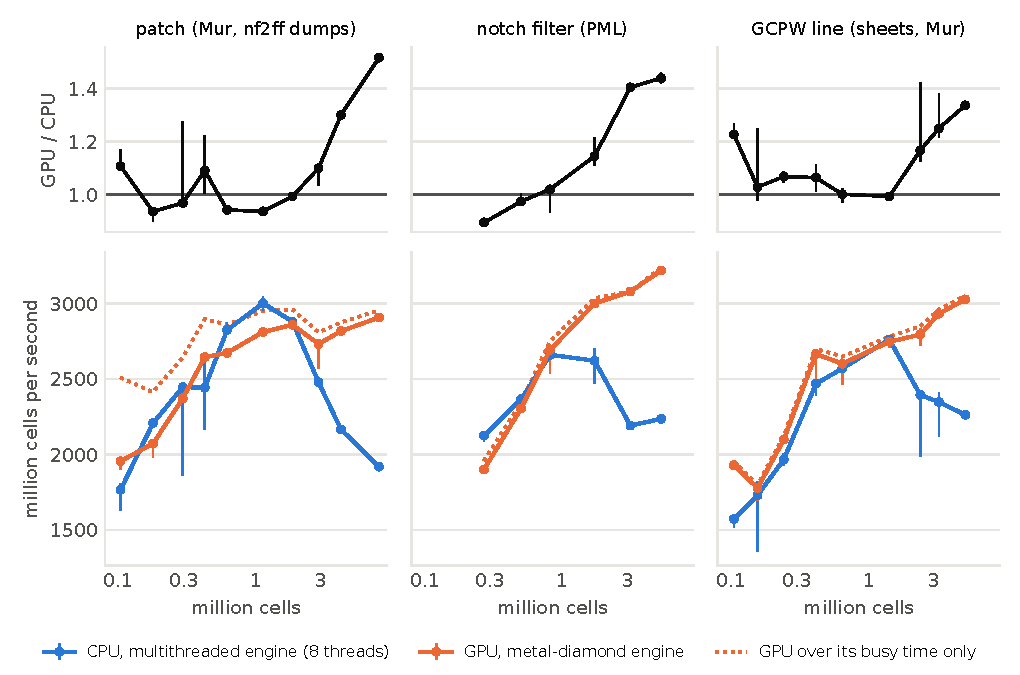
\includegraphics[width=\textwidth]{fig_crossover}
\caption{GPU against CPU by grid size on cg29 (\code{results/gpu\_crossover\_cg29\_2026-11-05.txt}). Top: the GPU
engine's speed over the multithreaded engine's at 8 threads, median of the paired rounds used and their range (4
rounds per point; 9 points rest on 3 and 2 on 2, see the text). Bottom: the medians in \MC\ with the range over the
same rounds; the dotted line is the GPU's rate over its busy time alone
(\code{OPENEMS\_DIAMOND\_TIMING=1}), so the gap down to the GPU's own line is time it waited for the CPU. The patch
and notch meshes are refined by the bench's scale factor (the tutorials at scale 1, patch x5 and notch x3 at scales 5
and 3); the GCPW line's scale multiplies its cell size (scale 1 is the 0.242\,M-cell line of the tables, scales 2 to
0.3 give 0.105 to 5.1\,M cells); logarithmic cell axis.}\label{fig:crossover}
\end{figure}

\paragraph{Tiles and $K$.} No one tiling is best for every model. In a sweep on cg23 (the faster of two runs, others'
CPU 0.4--2 cores, GPU up to 15\,\%) the default $K=4$ with 8:8 tiles was best or within 8\,\% on the four models built
from the tutorials and 8--9\,\% below the best setting on the two boards. In paired runs against the default the
SMA launch gained 1.132$\times$ [1.107--1.144] with $K=2$ and 6:4 tiles (cg24) and the GCPW line 1.114--1.117$\times$
per round with $K=4$ and 12:8 tiles (cg23; \code{results/diamond\_engine\_cg24\_cg27\_2026-11-04.txt}, section 8). The
run-time tuner of cg28 (above) chooses among four tilings. In the cg23 sweep four of the six models ran best with one
of them, and the SMA launch and the patch tutorial with a
$K=2$ tiling, 0.3 and 1.2\,\% faster than the best of the four; in a $K$ sweep on cg27 (the faster of two runs, not
paired; \code{results/fused\_sweep\_k1\_2026-11-04.txt}, part B) the default $K=4$ with 8:8 tiles beat $K=2$ with 4:4 tiles
and every $K=1$ tiling on all six models. $K=2$ with 6:4 tiles, the SMA launch's best in the paired runs of cg24
(against 1.065$\times$ for $K=3$ with 8:6 tiles), is not among the four, nor among the seven of cg31
(Section~\ref{sec:cg31}), and was not timed after cg24 up to cg29; the record of the sweep of thirteen tilings of
2026-11-11 does not list its tilings (\code{results/diamond\_engine\_cg28\_tuner\_2026-11-04.txt}, header;
\code{results/metal\_engine\_cg31\_2026-11-11.txt}).
The earlier fixed 1\,024 threads per tile cost 44\,\% on the notch tutorial and 21\,\% on the SMA launch against the
rule above (loaded Mac; \code{results/diamond\_engine\_cg21\_2026-11-04.txt}, section 4).

\paragraph{From cg24 to cg27.} The operator setup of cg24 runs on all cores: before it, the diamond engine set up
notch x3 in 5.55\,s and patch x5 in 6.48\,s, now in 2.74 and 1.69\,s, against 2.61 and 1.60 for the multithreaded
engine (loaded Mac; \code{results/diamond\_engine\_cg24\_cg27\_2026-11-04.txt}, section 5). A diagnostic build that
leaves parts of the work out (results not identical by design; 3 rounds) showed where the boards' time went: the SMA
launch ran 1.343$\times$ faster without the UPML, 1.257$\times$ with every cell on one operator and 1.167$\times$ without
the excitation, the GCPW line 1.514$\times$ without the sheets and 1.283$\times$ without Mur (section 7). The excitation
and the sheets became runs (cg25), the coefficients split tables (cg27); in one build, split against packed gave
1.053$\times$ [1.03--1.07] on the SMA launch and 1.031$\times$ [1.03--1.04] on the GCPW line (8 rounds, others 4--5
cores). Paired in one session against cg24 (5 rounds; others 4--5.6 cores, load average 11.7--25.2), cg27 ran the SMA
launch 1.265$\times$ [1.22--1.28] faster (median 1\,184 to 1\,482\,\MC) and the GCPW line 1.303$\times$ [1.29--1.37]
(1\,361 to 1\,773). The notch tutorial, notch x3 and patch x5 stayed within noise (0.983--1.012$\times$); the patch
tutorial's 1.251$\times$ [0.93--1.47] rests on 343 short calls under that load and is noise (section 3). Folding the
UPML stages into the cell update gave nothing (paired against cg24, 4 rounds: SMA launch 1.023$\times$
[0.934--1.106], notch tutorial 0.948$\times$, notch x3 0.988$\times$) and was removed (section 1).

\paragraph{Where the GPU waits.} With \code{OPENEMS\_DIAMOND\_TIMING} the engine reports its GPU time. On cg24 the GPU
was busy 96--99\,\% of the time-stepping loop on the two boards and notch x3 and 91\,\% on patch x5, but 78\,\% on the
patch tutorial and 76\,\% on the notch tutorial, whose \code{IterateTS} calls are short (31 steps between the patch
tutorial's nf2ff dumps, 81 on the notch tutorial) and leave the GPU idle while the CPU works between them. On cg29, in
the size sweep above, the patch tutorial kept the GPU busy 79--82\,\% of the loop (73--79\,\% in later runs), but the
notch tutorial 97\,\% with the same 81-step calls: its cg24 figure, from a loaded Mac, was not reproduced. Timed per
phase, notch x3 spent 12/17/18/53\,\% of the GPU time in the four kinds of tile, against a work split of
10/18/18/54\,\% at $M=V=8$, $K=4$: per cell update the four cost the same
(\code{results/diamond\_engine\_cg24\_cg27\_2026-11-04.txt}, section 6).

\paragraph{The run-time tuner (cg28).} Table~\ref{tab:gpuspeed}(a) gives the paired comparison with cg27 on a quiet
Mac: 1.094$\times$ on the SMA launch, 1.114$\times$ on the GCPW line, 1.061$\times$ on notch x3 and 1.064$\times$ on
the patch tutorial. On the notch tutorial and patch x5 the default is the best tiling; there the tuning, 575 and 623
steps with the other tilings in turn, costs 0.4--0.5\,\% of these short runs, and less in real runs of 34\,000 to
190\,000 steps. The choices were those of the best fixed tiling in the paired sweeps and the same in every repeat
(\code{results/diamond\_engine\_cg28\_tuner\_2026-11-04.txt}, sections 2 and 3).

\paragraph{Fused but not blocked ($K=1$).} At $K=1$ a threadgroup updates the voltages and then the currents of its
tile in one pass, and the four kinds of tile complete the tile edges, so each field value is read and written once
per step: the 49\,B per cell of the CPU's fused sweep, the case that Section~\ref{sec:ceiling} bounds at
2\,470--2\,590\,\MC. Measured on cg27 (Table~\ref{tab:gpuspeed}(b); paired, 4 rounds, others' CPU 2.5--4 cores, GPU
3--5\,\%), it ran notch x3 at 1\,716--1\,733\,\MC\ and patch x5 at 1\,530--1\,844 over three tile sizes, 0.54--0.65
times $K=4$. At each model's best tile that is 1.25--1.30 times the base's unfused GPU engine (ratio of the medians),
67--75\,\% of the bound, and 85--90\,GB/s at 49\,B per cell, where the streaming kernels drew 121--127\,GB/s; against
the CPU best of cg18 on a quiet Mac, a comparison across sessions, it is 0.85 (notch x3) and 1.07 times (patch x5)
(\code{results/fused\_sweep\_k1\_2026-11-04.txt}). The per-step structure (four dispatches, the tile edges, a
threadgroup barrier between the two half steps) costs more than the bytes it saves; the bound is a traffic bound only.
Blocking over time steps does what fusing alone does not: $K=2$ (2\,123 and 2\,408\,\MC) is still below the bound,
$K=4$ (2\,986 and 2\,817) above its upper end on both models. A one-dispatch fused kernel was not built: tiles that
compute their own edges would overwrite values their neighbours still read in the same dispatch, so it needs a second
copy of both fields, and every extension would have to follow.

\paragraph{End to end.} Through the author's toolkit (cg23; one run each, another session's job on one core, load
average 2.6--8.0) the engine cut the toolkit's default runs (probe end $-60$\,dB, hold 0.5) from 7.43 to 5.95\,s on
the GCPW line (1.25$\times$) and from 43.71 to 34.23\,s on the SMA launch at 0.871\,M cells (1.28$\times$), and the
full runs to \code{max\_time} by 1.15$\times$ and 1.26$\times$ (\code{FDTD.Run} wall time), against the multithreaded
engine of the same build with its automatic thread count (\code{results/rfsim\_e2e\_gpu\_2026-11-04.txt}). On cg27, under a heavier load, the GPU
runs gave the same port data (\code{results/diamond\_engine\_cg24\_cg27\_2026-11-04.txt}, section 9). The end-to-end
runs of cg29 are in Section~\ref{sec:results}.

\begin{table}[htbp]\centering\small
\textbf{(a)} cg28 (tiling chosen at run time) against cg27, paired, 5 rounds; quiet Mac (others' CPU 0.5--1.3 cores,
GPU 2--4\,\%)\\[3pt]
\resizebox{\textwidth}{!}{%
\begin{tabular}{@{}lrrllll@{}}
\toprule
model (cells, steps) & cg27 & cg28 & cg28 / cg27 & \code{TUNE=0} / cg27 & tiling chosen & tuning steps \\
\midrule
SMA launch (0.871\,M, 6000)      & 1671 & 1828 & 1.094 [1.092--1.097] & 1.001 [0.999--1.003] & $K=3$, 8:6  & 584 \\
GCPW line (0.242\,M, 15000)      & 1896 & 2113 & 1.114 [1.068--1.117] & 0.999 [0.963--1.003] & $K=4$, 12:8 & 588 \\
notch x3 (5.247\,M, 3000)        & 3039 & 3226 & 1.061 [1.061--1.064] & 0.998 [0.996--1.000] & $K=4$, 12:8 & 614 \\
patch tutorial (0.104\,M, 10500) & 1640 & 1764 & 1.064 [1.010--1.152] & 1.000 [0.942--1.042] & $K=3$, 6:6  & 532 \\
notch tutorial (0.270\,M, 16000) & 1908 & 1902 & 0.996 [0.994--1.001] & 0.998 [0.994--1.002] & $K=4$, 8:8  & 575 \\
patch x5 (7.863\,M, 2400)        & 2930 & 2917 & 0.995 [0.994--0.997] & 1.003 [1.002--1.005] & $K=4$, 8:8  & 623 \\
\bottomrule
\end{tabular}}

\vspace{8pt}
\textbf{(b)} The fused, unblocked sweep ($K=1$) on cg27, paired, 4 rounds (others' CPU 2.5--4 cores, GPU 3--5\,\%);
\MC\ (ratio to $K=4$)\\[3pt]
\resizebox{\textwidth}{!}{%
\begin{tabular}{@{}lrrrrrr@{}}
\toprule
model (cells) & base GPU engine (unfused) & $K=1$, 8:8 & $K=1$, 16:8 & $K=1$, 32:16 & $K=2$, 4:4 & $K=4$, 8:8 \\
\midrule
notch x3 (5.247\,M) & 1330 (0.446) & 1716 (0.573) & 1729 (0.579) & 1733 (0.579) & 2123 (0.710) & 2986 \\
patch x5 (7.863\,M) & 1469 (0.515) & 1799 (0.637) & 1844 (0.649) & 1530 (0.541) & 2408 (0.852) & 2817 \\
\bottomrule
\end{tabular}}
\caption{Speed of the Metal diamond engine, \MC\ (medians of the rounds; a ratio is the median of the per-round
ratios, with its range). Tiles are $M$:$V$. (a) \code{results/diamond\_engine\_cg28\_tuner\_2026-11-04.txt}, section 3;
the tiling chosen and the steps the tuning took come from one separate run per model (section 2; others about 0.5--1
core), and the choice was the same in every repeat. \code{TUNE=0} is cg28 with \code{OPENEMS\_DIAMOND\_TUNE=0}, the
fixed $K=4$, 8:8 of cg27. (b) \code{results/fused\_sweep\_k1\_2026-11-04.txt}, part A. The base GPU engine is
\code{--engine=gpu} of the fork's base (7bb294f), not upstream master's merged engine. The traffic bound of a fused
sweep at 49\,B per cell is about 2\,470--2\,590\,\MC\ (Section~\ref{sec:ceiling}). Every run of both sessions equals
its session's first run, and so the multithreaded engine with \code{OPENEMS\_FTZ=1}.}
\label{tab:gpuspeed}
\end{table}

\subsection{Limits and open questions}
\begin{itemize}
\item \textbf{One machine.} Everything here ran on the base M5 with its 10 GPU cores, whose bus the CPU shares. The M5
  Pro (307\,GB/s~\cite{macmini}) was measured later, with cg31, as a set of its own (Section~\ref{sec:m5pro}); the M5
  Max and the M5 Ultra (1.2\,TB/s~\cite{studiom5}) were not measured; for
  luikore's engine, 1.3--4.2$\times$ its own unfused path is reported on an M4 Pro and an M5 Max~\cite{luikore228}.
\item \textbf{No head-to-head with luikore's engine on the six models.} On this M5 its diamond path refused all six
  models (Mur faces; on the GCPW line also the conducting sheets) and ran only variants with every Mur face replaced
  by PEC, on which this engine was not run (\code{results/others\_2026-11-04/}, Section~\ref{sec:ceiling}). Since
  2026-11-11 there is one on luikore's own benchmark model, a uniform grid with PEC walls: cg31's engine ran 3\,981
  and 3\,309\,\MC\ at 3.0 and 17.0\,M cells, luikore's 3\,952 and 2\,829 (Section~\ref{sec:threebuilds},
  Table~\ref{tab:threebuilds}). Its diamond path still refuses the six models.
\item \textbf{No bytes per cell.} The traffic model of Section~\ref{sec:fused} gives the bytes of a sweep that streams
  every array once or twice per step. With $K$ steps per tile the traffic depends on what the caches keep, and it was
  not measured with hardware counters, so this engine has no bytes-per-cell figure and no bar in
  Figure~\ref{fig:bandwidth}. Its rates above the bound show only that it moves less than 49\,B per cell update.
  Section~\ref{sec:cg31} adds a count from the tile schedule, 20--29\,B of field per cell and step for a tile that
  stays cached through its block; it is a count, not a measurement.
\item \textbf{GPU memory} was not measured: the shared field buffers, the four tilings' buffers while tuning (seven
  tilings since cg31), the extension buffers. Only the coefficient tables are known (above).
\item \textbf{Graded meshes and extension work.} The boards run below the large uniform models, for their UPML, sheet
  and excitation work and their many distinct operators (the ablation above), and for their size: refined to 3.2 and
  5.1\,M cells, the GCPW line ran between patch x5 and notch x3 (Figure~\ref{fig:crossover}). The SMA launch,
  1\,829\,\MC\ at 1.07\,M cells in Table~\ref{tab:current} against 2\,747--2\,812 for the GCPW line and the patch
  antenna at 1.1--1.4\,M cells in the size sweep (another session), was not scaled. The tuner picks among four tilings
  only. Since cg31 (Section~\ref{sec:cg31}) a block takes three dispatches, the UPML and the dispersive stages take a
  z-vector or the three components of a cell at a time, Mur faces of one axis share a barrier and the tuner has seven
  tilings: the GCPW line and the SMA launch (0.871\,M cells) gained 1.09$\times$ and 1.14$\times$
  (Table~\ref{tab:cg31}). The extensions still cost, and the cost is tied to their code being compiled into the
  kernel, not to the loops over their cells; that is not explained.
\item \textbf{Coverage.} TFSF, steady-state detection and subclasses of the dispersive extensions put a model on the
  one-thread CPU loops; probes and dumps run on the CPU between calls, which, with the start and finish of each call's
  command buffers, left the GPU idle for about a quarter of the loop on the two tutorials at cg24, and at cg29 still for 18--27\,\% on the patch tutorial (3\,\% on the notch
  tutorial; Figure~\ref{fig:crossover}). Up to cg29 the engine also waited for the base's energy estimate, one CPU
  thread over both fields every Nyquist period of a run's first 60\,s; since cg31 a run without an end criteria makes
  none (Section~\ref{sec:cg31}).
\item \textbf{fp16 field storage} was not tried: late-run currents of $10^{-6}$\,A lie below the half-precision normal
  range, which ends at $6\times10^{-5}$ (project log), so the fields would need scaling, and the result could not be
  bit-identical.
\item \textbf{Load.} The speeds of cg19 to cg27 and of the $K=1$ runs come from a loaded Mac (each with its load
  above). Of the GPU-against-GPU comparisons of this section only cg28's is quiet (that of cg31 with cg29,
  Table~\ref{tab:cg31}, ran with the other sessions paused); the GPU against the CPU engine and stock is
  Table~\ref{tab:current}, and against the CPU engine by grid size the size sweep, which waited for a quiet Mac
  before every run; its ratios on grids below 0.3\,M cells still moved by up to 16\,\% between sessions.
\end{itemize}

\section{The modelling side: shorter runs for the same answer}\label{sec:modelling}

Once the engine is at the bus, a run's wall time is cells $\times$ time steps $\div$ speed, and the first two are
set by the model and by openEMS's time-step criterion. Three changes act there; all live in the author's simulation
toolkit (rfsim) except the end criterion, which is in openEMS. The changes made to the toolkit in this project are not
published, since the toolkit itself is private; this section and \code{CHANGELOG.md} describe them.

\subsection{A run-end criterion on the port probes}\label{sec:probeend}
openEMS stops a run when the total field energy has fallen below a threshold relative to its peak (default
$-50$\,dB) or at a maximum number of steps or time. On both boards the energy criterion never fires: a Gaussian
pulse has a DC component, the open structure stores it as a static charge, and the energy stays far above the
threshold. At the end of the full runs of Table~\ref{tab:probeend} it still reads $-11.1$\,dB (SMA) and $-14.9$\,dB
(GCPW) of its peak (\code{results/rfsim\_e2e\_2026-11-03.txt}), while every port signal is below $-80$\,dB of its
peak after about a quarter of the run. Runs therefore always went to \code{max\_time}, and the toolkit proved
settling after the fact from the port files. Upstream master has since added an opt-in DC-free Gaussian pulse (commit
d686f1d, 2026-10-24: \code{SetGaussExcite(f0, fc, dc\_free=True)}, a sine instead of a cosine carrier); it is not in
v0.37.0 or in the fork's base. It leaves no static charge, so the energy criterion can fire, but it changes the
excitation: its spectrum falls to zero at DC, so the bottom of the band (50\,MHz for these boards) is driven more
weakly. The criterion below keeps the model and its pulse as they are.

The fork adds a second criterion, off unless \code{OPENEMS\_PROBE\_END\_DB} is set to a negative level in dB; an
invalid value of it or of \code{OPENEMS\_PROBE\_END\_HOLD} prints a warning. Every integral probe (port voltages and
currents, field probes) tracks the largest absolute value it has seen and its latest value; a waveguide
(mode-matching) probe counts with its mode amplitude only, not its mode purity. At every step at which one of the
processings runs (a probe or dump sample, or an energy estimate; on the GCPW line the probes sample every 490 steps, a
quarter of the Nyquist interval), the engine computes the worst ratio latest/peak over all probes, so a run can only
stop on such a step. It stops once that ratio has stayed below the threshold for a hold time of
\code{OPENEMS\_PROBE\_END\_HOLD} excitation lengths (default 1). The hold starts again at every check at which a
probe is above the threshold, a probe has seen no signal yet (its peak is still exactly zero), or the excitation is
still running; the excitation counts as running until the end of its signal plus the largest excitation delay, taken
over every grid (the child grids of a cylindrical multigrid included) and including the propagation delay of a
total-field/scattered-field (TFSF) source. A probe that never sees a signal holds the run to its end; once all the
others have settled, a one-time notice names it. A far probe can pick up tiny numerical precursors shortly before the
pulse arrives, and those count as a signal, so the hold should be longer than the longest one-way delay from the
excitation to a probe. A probe whose own peak is below $10^{-6}$ of the largest peak of its kind (a current probe on an
open end, say) is measured against $10^{-6}$ of that largest peak instead of its own near-zero peak. The criterion
needs a Gaussian excitation and at least one probe; if either is missing it prints a warning and ignores the setting.
The time-domain probe and port files of a stopped run are a bit-identical prefix of the full run's (checked for every
stopped run of Table~\ref{tab:probeend}; only the stop point changes); frequency-domain dumps and nf2ff data are sums
over the shorter record and change accordingly. The toolkit sets the variables around every \code{FDTD.Run()}: by
default \code{probe\_end\_db=-60} and, since toolkit commit 4a7e20e of 2026-11-04, \code{probe\_end\_hold=0.5}
(\code{RFSIM\_PROBE\_END\_HOLD=1} restores the earlier default of 1).
Table~\ref{tab:probeend} shows the effect on both boards.

\begin{table}[H]\centering\small
\resizebox{\textwidth}{!}{\begin{tabular}{@{}llrrl@{}}
\toprule
model & setting & steps & time & change vs the full run \\
\midrule
GCPW line, 12\,ns & full run (max\_time) & 94\,217 & 13.7\,s & -- \\
 & $-60$\,dB, hold 1 & 45\,570 & 8.6\,s & $S_{21}$ $8.0\times10^{-4}$\,dB, $S_{11}$ $1.3\times10^{-4}$ lin., $Z_0$ $-0.0003\,\Omega$ \\
 & $-80$\,dB, hold 1 & 47\,040 & 7.1\,s & $S_{21}$ $7.9\times10^{-4}$\,dB, $S_{11}$ $1.2\times10^{-4}$ lin., $Z_0$ $-0.0009\,\Omega$ \\
 & $-60$\,dB, hold 0.5 & 34\,300 & 5.2\,s & $S_{21}$ $7.1\times10^{-4}$\,dB, $S_{11}$ $2.2\times10^{-4}$ lin., $Z_0$ $-0.0005\,\Omega$ \\
\addlinespace
SMA launch, 10\,ns & full run (max\_time) & 182\,622 & 168.5\,s & -- \\
 & $-60$\,dB, hold 1 & 103\,831 & 97.6\,s & $S_{11}$ 0.0089\,dB at $-22.8$\,dB, $S_{21}$ $2.3\times10^{-4}$\,dB, $Z_0$ $-0.0066\,\Omega$ \\
 & $-80$\,dB, hold 1 & 106\,113 & 99.8\,s & $S_{11}$ 0.0100\,dB, $S_{21}$ $1.9\times10^{-4}$\,dB, $Z_0$ $-0.0037\,\Omega$ \\
 & $-60$\,dB, hold 0.5 & 77\,588 & 72.9\,s & $S_{11}$ 0.0188\,dB, $S_{21}$ $2.2\times10^{-4}$\,dB, $Z_0$ $-0.0092\,\Omega$ \\
\bottomrule
\end{tabular}}
\caption{Probe end criterion on the two boards: cg18, automatic thread count, one run each, measured on 2026-11-03
(\code{results/rfsim\_e2e\_2026-11-03.txt}); the SMA launch on the 1.071\,M-cell mesh of the toolkit's former
0.02\,mm floor ($\Delta t$ 54.76\,fs). On the GCPW line the $-60$\,dB, hold 0.5 row is the toolkit's
default run since 2026-11-04; on the SMA launch that default also has the 0.05\,mm mesh floor (Table~\ref{tab:mesh}).
Time: wall time of \code{FDTD.Run} (operator setup and time stepping). Changes against the
full run of the same board, the largest over 50\,MHz--2\,GHz: $|\Delta S_{21}|$ in dB; $|\Delta S_{11}|$ linear on the
GCPW line (its $S_{11}$ stays below $-40$\,dB) and in dB where $|S_{11}|>-40$\,dB on the SMA launch; $\Delta Z_0$ is
the change of $\mathrm{Re}\,Z_0$ at 640\,MHz (GCPW) and 1\,GHz (SMA). In the GCPW's $-60$\,dB, hold 1 run the tuner
picked 8 threads (1\,304\,\MC, against 1\,636--1\,683\,\MC\ at 4 threads in the other fdtdKit GCPW runs), so it took
longer than the $-80$\,dB run, which has more steps.}\label{tab:probeend}
\end{table}

\subsection{z lines in multiples of four}
The SSE engines pack four z lines per vector and compute $4n_v$ slots per $(x,y)$ column ($n_v=\lceil N_z/4\rceil$
z-vectors; the spare slots are the top lane of the last z-vectors), so a board with 17 z lines costs the time of 20.
The toolkit can now halve the largest z cell (the air above the board) until the line count is a multiple of four; it
never splits the boundary cells at z max (one for Mur, $N$ for PML\_$N$) and never shrinks the time step. The GCPW
line goes from 17 to 20 lines and from 0.242 to 0.285 million cells in the \emph{same} wall time (bench: 1.13\,s versus
1.10\,s for 8\,000 steps at 4 threads), with the time step unchanged. It is a finer mesh, so results move, by
$5\times10^{-5}$ relative in the probes and $10^{-4}$\,dB in $S_{21}$; it is opt-in. These numbers are from the
project log, not in \code{results/}, and were taken with the first version of the padding, which also split the top
boundary cell; the toolkit's current version keeps that cell, so its mesh differs at the top (the line count, and
with it the timing, is the same). Rounding down instead, by dropping the top-most air line (17 to 16 lines), would save one
z-vector of run time, but it lowers the lid by one air cell: a change of the model rather than of its mesh, left to
the toolkit's user.

\subsection{A minimum cell size for the SMA launch}\label{sec:meshfloor}
The SMA launch has 69\,500 distinct operators and, on the toolkit's original mesh (that of 2026-10-17), a time step
of 53.0\,fs set by cells of 0.025--0.045\,mm (operator count and cell sizes from the project log, the time step from
\code{results/sma\_mesh\_sweep\_2026-11-01.txt}). Those cells are not design intent: they are where a tangent line of
the pin, the PTFE bore or a via edge lands 0.025--0.045\,mm from a line of the regular 0.075 or 0.15\,mm grids. The
builder merged lines closer than 0.02\,mm by keeping the first; it now takes a \code{min\_cell} floor and merges with
priorities: strip and gap lines (the port's $1/3$--$2/3$ edge rule) always stay, a geometry line wins over a grid
line, and two geometry lines meet in the middle so the error is split. The first core cell under the top plane also
starts at the floor.

A first version of this merge was swept on 2026-11-01 (engine cg16, against the full run on the original mesh; the
first table of \code{results/sma\_mesh\_sweep\_2026-11-01.txt}). At 0.06\,mm the four-cell prepreg lost two of its
cells and $S_{11}$ moved by up to 3.3\,dB ($-19.98$ against $-22.80$\,dB at 1\,GHz); the last row of
Table~\ref{tab:mesh} keeps that run as history. The pre-publication review of this change then found two bugs in
that first merge. The floor was not multiplied by the model's \code{scale} factor, so the 0.6 convergence mesh was
merged with the unscaled floor and the coarse/fine pair was no longer a convergence pair; and the merge scanned the
lines from $-y$ to $+y$, so chains of three or more close lines resolved differently on the two sides and a
mirror-symmetric structure got an asymmetric mesh at every floor above 0.02\,mm. The merge is now independent of the
scan order (\code{core.merge\_lines}): protected lines never move and are never merged; a pair or a short run of
geometry lines closer than the floor is replaced by its mean, and a longer run (a grid finer than the floor) is
thinned to evenly spaced lines at least the floor apart; grid lines give way; and the builder refuses a floor that is
not below every fixed cell of the stack-up or the strip rule (0.0526\,mm and above for this board, 0.06\,mm included).

The 0.02\,mm mesh, the toolkit's default until 2026-11-04, is the same line for line with both merges; against
the original mesh it differs in the 14 lines that the caption of Table~\ref{tab:mesh} lists, and its time step is
54.76\,fs instead of 53.0\,fs. With the corrected merge the 0.04 and 0.05\,mm meshes gained lines (0.953 and 0.871
million cells; the first merge had dropped lines asymmetrically). A sweep of these meshes on 2026-11-02 ran while
other simulations loaded the machine, so its run times could only be estimated. Figure~\ref{fig:mesh} and
Table~\ref{tab:mesh} give the sweep measured on 2026-11-03 with cg18 and the corrected merge, against the full run on
the 0.02\,mm mesh; it reproduces the step counts of 2026-11-02 exactly and replaces the estimated
times. The suggestion stands: 0.05\,mm with a hold of 0.5 needs 2.54 times fewer cell-steps and 2.61 times less run
time than the earlier defaults (the 0.02\,mm mesh with a hold of 1; 37.4\,s against 97.6\,s), with $S_{11}$ within
0.12\,dB at $-22.8$\,dB and $Z_0$ 0.12\,$\Omega$ higher; with a hold of 1 the floor alone gives 1.90 and 1.97 times
(49.5\,s). That error is far inside the 30\,dB return-loss bench floor the model documents for itself: an error wave
30\,dB below the incident one, on a reflection of $-22.8$\,dB, allows any reading from $-19.7$ to $-27.8$\,dB. The
author adopted it on 2026-11-04: since toolkit commit 4a7e20e the toolkit's defaults are the 0.05\,mm floor
(0.871\,million cells on this board) and a hold of 0.5 for every run, and \code{RFSIM\_MIN\_CELL=0.02} and
\code{RFSIM\_PROBE\_END\_HOLD=1} restore the old ones.

\begin{table}[H]\centering\small
\resizebox{\ifdim\width>\textwidth\textwidth\else\width\fi}{!}{\begin{tabular}{@{}lrrrrrrr@{}}
\toprule
floor & cells & $\Delta t$ & steps & run & $S_{11}$ at 1\,GHz & $\max|\Delta S_{11}|$ / $|\Delta S_{21}|$ & $\Delta Z_0$ \\
\midrule
0.02\,mm$^{\dagger}$ & 1.071\,M & 54.8\,fs & 103\,831 & 97.6\,s & $-22.80$\,dB & 0.0089 / 0.0002\,dB & $-0.007$\,$\Omega$ \\
0.03\,mm & 1.007\,M & 58.5\,fs & 97\,097 & 85.7\,s & $-22.79$\,dB & 0.0292 / 0.0006\,dB & +0.03\,$\Omega$ \\
0.04\,mm & 0.953\,M & 78.0\,fs & 72\,891 & 58.0\,s & $-22.72$\,dB & 0.0782 / 0.0014\,dB & +0.12\,$\Omega$ \\
0.05\,mm & 0.871\,M & 84.4\,fs & 67\,340 & 49.5\,s & $-22.69$\,dB & 0.1156 / 0.0021\,dB & +0.10\,$\Omega$ \\
0.02\,mm, hold 0.5 & 1.071\,M & 54.8\,fs & 77\,588 & 72.9\,s & $-22.80$\,dB & 0.0188 / 0.0002\,dB & $-0.009$\,$\Omega$ \\
0.05\,mm, hold 0.5$^{*}$ & 0.871\,M & 84.4\,fs & 50\,320 & 37.4\,s & $-22.69$\,dB & 0.1157 / 0.0021\,dB & +0.12\,$\Omega$ \\
\midrule
\multicolumn{8}{@{}l@{}}{\emph{history: first merge, 2026-11-01 (engine cg16; see the caption)}} \\
0.06\,mm & 0.625\,M & 130.1\,fs & 43\,680 & 24.3\,s & $-19.98$\,dB & 3.292 / 0.0237\,dB & +0.43\,$\Omega$ \\
\bottomrule
\end{tabular}}
\caption{SMA launch mesh floor sweep, 10\,ns, probe end $-60$\,dB with a hold of 1 unless stated, measured on
2026-11-03 with cg18 (the tuner picked 8 threads in every run), one run each, with the corrected merge (the
2026-11-03 section of \code{results/sma\_mesh\_sweep\_2026-11-01.txt}; the same runs as in
\code{results/rfsim\_e2e\_2026-11-03.txt}). Run: wall time of \code{FDTD.Run}. Changes against the full run on the
0.02\,mm mesh (182\,622 steps of 54.76\,fs, Table~\ref{tab:probeend}): $\Delta S_{11}$ in dB where
$|S_{11}|>-40$\,dB over 50\,MHz--2\,GHz, $\Delta S_{21}$ the largest over that band, $\Delta Z_0$ the change of
$\mathrm{Re}\,Z_0$ at 1\,GHz (to 0.01\,$\Omega$ where it exceeds 0.01\,$\Omega$). $^{\dagger}$The toolkit's default
until 2026-11-04 (with a hold of 1). $^{*}$The toolkit's default since 2026-11-04 (toolkit commit 4a7e20e).
The first row's mesh differs from the toolkit's original mesh (that of 2026-10-17: 188\,697 steps of 53.0\,fs for
10\,ns) in 14 lines: nine move by at most 0.01\,mm (four in x, five in y) and five y lines between 3.6 and 4.45\,mm by
up to 0.10\,mm, where the original y mesh was not mirror-symmetric. The last row is history: the 0.06\,mm run of the
first merge (2026-11-01, against the full run on the original mesh; the first table of the same file), in which the
four-cell prepreg lost two of its cells; the builder refuses that floor now.}\label{tab:mesh}
\end{table}

\begin{figure}[htbp]\centering
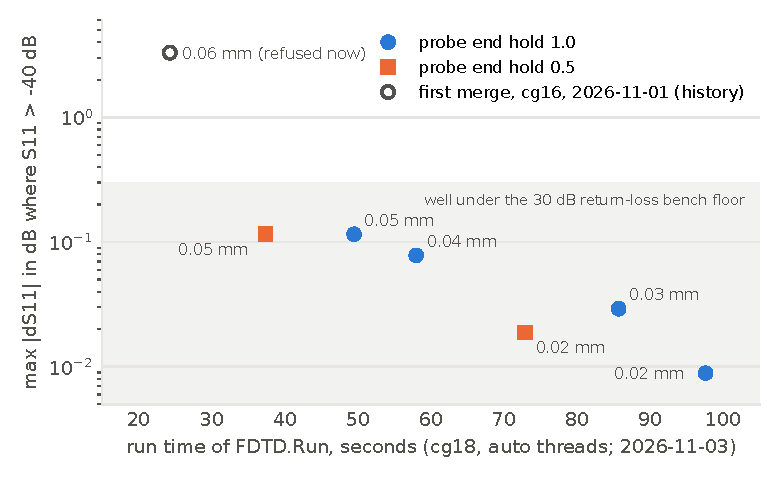
\includegraphics[width=0.62\textwidth]{fig_mesh}
\caption{Run time against the $S_{11}$ error for the mesh floors of Table~\ref{tab:mesh}, measured on 2026-11-03 with
cg18 and the corrected merge. The hollow grey point is history: the 0.06\,mm run of the first
merge (2026-11-01, engine cg16, against the full run on the original mesh), a floor the builder now
refuses.}\label{fig:mesh}
\end{figure}

\section{Results}\label{sec:results}

\subsection{Engine speed}
Figure~\ref{fig:speed} compares stock and snapshot cg14 on the six models: fdtdKit at each model's best thread count,
stock at its best for the four tutorial models and at 4 threads for the two boards, whose stock thread count was not
swept. Figure~\ref{fig:progress} shows how the speed-up accumulated snapshot by snapshot (Table~\ref{tab:snapshots}
names them); Figure~\ref{fig:threads} and Table~\ref{tab:final} give the thread scaling of cg14 and the automatic
choice. These engine-speed figures and tables stop at cg14. Snapshot cg18 (patches 0001--0006, the build installed on
the author's Mac from 2026-11-04 to 2026-11-06) went through the same full check on a quiet machine on 2026-11-03
(\code{results/*\_cg18.txt}):
bit-identical to stock on all six
models; its best speeds differ from cg14's by $-2.7$ to $+1.6$\,\% on five models and by $+8.2$\,\% on the GCPW line
(whose cg13 run had reached 1\,745\,\MC); on the four models of up to about a million cells it reaches
1\,361--1\,961\,\MC, 3.1--6.8$\times$ the stock rows of the same tables. The cg17 tables in \code{results/} are
correctness checks, run while the machine was loaded. The current build, cg29, is compared with stock on the CPU and
on the Metal diamond engine in Section~\ref{sec:current}.

Part of the patch tutorial's factor is not the patches' (\code{results/*\_base.txt}, 2026-11-03, best of two runs on
a quiet machine). The fork's base, upstream's \code{gpu-engine} branch at 7bb294f with stock's CSXCAD and nf2ff
libraries, runs that model 1.13$\times$ faster than stock (308.5 against 273.4\,\MC, both at their best, 2 threads),
all of it on the dump side: with the dumps off both reach 342.2\,\MC\ at 2 threads. The difference is the base's
background HDF5 writer, which writes the model's 12 time-domain dumps off the main thread and keeps their files open
(the CPU engines still evaluate the dumps on the main thread; only the base's GPU engine evaluates them from a field
snapshot, and the Metal diamond engine of Section~\ref{sec:gpu} leaves them to the CPU between its calls). Snapshot
cg18 runs that model 5.98$\times$ faster than the base (1\,845.9\,\MC\ at 4 threads), so the
patches' own factor there is about 6.0$\times$. On the notch tutorial, the GCPW line and patch x5 the base runs within
0.98--1.03$\times$ of stock; the SMA launch was not run with it. Every run in these files has stock's probes and
$S$-parameters.

\begin{figure}[htbp]\centering
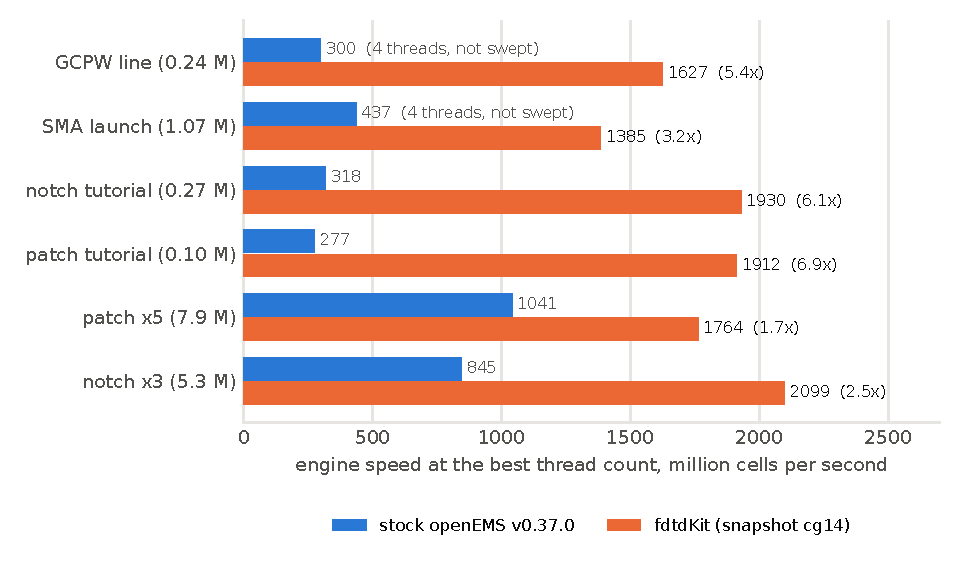
\includegraphics[width=0.9\textwidth]{fig_speed}
\caption{Stock v0.37.0 against fdtdKit snapshot cg14 (\code{results/*\_cg14.txt}), same results bit for bit. fdtdKit at
each model's best thread count; stock at its best for the tutorial models (Table~\ref{tab:step1}) and, for the two
boards, one 4-thread reference run each (the cg10 run for the GCPW line, the cg14 run for the SMA launch), as their
stock thread count was not swept. On the patch tutorial about 1.13$\times$ of the factor comes from the fork's base
(see the text).}\label{fig:speed}
\end{figure}

\begin{table}[p]\centering\footnotesize
\begin{tabular}{@{}lp{0.82\textwidth}@{}}
\toprule
snapshot & added \\
\midrule
A & spin barriers, hook plan \\
AB & + inner loop (IJKN) \\
ABCDEG & + work stealing, automatic thread count (0.15\,s windows), Mur fast path, UPML on vectors, fused sweep with
line hooks for Mur, UPML, excitation and lumped RLC, background HDF5 writer \\
cg, cg2 & rebased on upstream's gpu-engine branch at commit 7bb294f (its gather and asynchronous dumps; the branch has
since been deleted upstream), slab balancing; Field\_Gather\_SSE \\
cg6 & Mur line hooks vectorised in memory order (from cg4; the dump experiments of cg3 and cg5 removed) \\
cg8 & thread tuner timed in pieces of window/8 with slab balancing between them (cg7), refined search \\
cg9 & threaded operator setup, nf2ff matrix product, CSXCAD lookups, operator/field export \\
cg10 & staggered allocations (allocation-placement valley), \code{--disable-dumps} crash fix \\
cg11 & scalar-SSE UPML path for z-only PML slabs \\
cg12 & line hooks for the dispersive extensions (conducting sheets) \\
cg13 & packed coefficient tables \\
cg14 & compressed UPML coefficient tables \\
cg15 & user-initiated thread QoS \\
cg16 & probe end criterion \\
cg17 & review fixes (patch 0005): Debye hooks, probe end arming, setup cache key, portability guards
(Section~\ref{sec:reviewfixes}) \\
cg18 & final-review fixes (patch 0006): probe end with excitation delays and waveguide probes, packed tables always
built, on/off switches, tuner clamp, flush-to-zero state restored, size limits (Section~\ref{sec:reviewfixes}) \\
cg19 & Metal diamond engine, \code{--engine=metal-diamond} (0007): cell updates, excitation and Mur on the GPU
(Section~\ref{sec:gpu}) \\
cg20 & + lumped RLC elements on the GPU (0008) \\
cg21 & + UPML on the GPU; extension data in three buffers; threads per tile from the tile size (0009) \\
cg22 & + Drude/Lorentz materials and conducting sheets on the GPU: all six models run there (0010) \\
cg23 & + Debye materials on the GPU (0011) \\
cg24 & GPU engine's operator setup on all cores (\code{Operator\_Multithread}); \code{OPENEMS\_DIAMOND\_TIMING} (0012) \\
cg25 & excitation and dispersive elements as runs; per-tile offsets read once (0013) \\
cg26 & grid sizes as constants of the kernel; Mur and UPML records passed by value (0014) \\
cg27 & split coefficient tables for graded meshes (0015) \\
cg28 & tiling chosen at run time (0016) \\
cg29 & CPU items (0017--0027, one per topic; Section~\ref{sec:cg29}): operator index per z-vector, merged ADE for
conducting sheets, UPML y-rows, UPML setup on the setup threads (PR \#244), line hooks for the steady-state detection
and for Debye materials, geometry coefficient tables, \code{OPENEMS\_FUSED\_STAT}, neighbour flags instead of the two
barriers with RLC slots by time step (Discussion \#492), steady-state detection on the flags, no flag spin above the
P-core count \\
\bottomrule
\end{tabular}
\caption{Snapshots. Each is a complete set of dylibs plus the cumulative patch, kept for bisection on the author's
machine. \code{patches/openems/} publishes the fork as patches 0001--0027: 0001--0006 end at cg18 (0001 = cg8, 0002 =
cg9, 0003 = cg10--cg15, 0004 = cg16, 0005 = cg17, 0006 = cg18), the build installed on the author's Mac from
2026-11-04 to 2026-11-06; 0007--0016 are cg19--cg28, one per snapshot (Table~\ref{tab:gpucov}); 0017--0027 are cg29,
one per topic (Table~\ref{tab:cg29}), the build installed there since 2026-11-06. A row lists what the snapshot added
over the row above; the intermediate snapshots cg3--cg5 and cg7 appear inside the cg6 and cg8
rows.}\label{tab:snapshots}
\end{table}

\begin{figure}[htbp]\centering
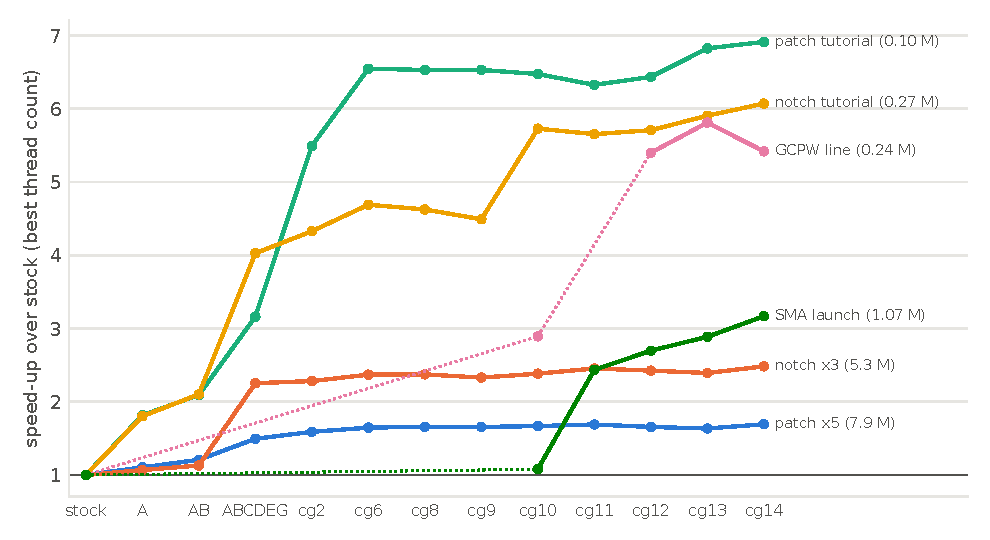
\includegraphics[width=0.95\textwidth]{fig_progress}
\caption{Speed-up over stock per snapshot (the best thread count of each check run; \code{results/summary.json}, which
\code{paper/figures/parse\_results.py} collects from the tables in \code{results/}). Stock as in
Figure~\ref{fig:speed}. The two boards joined the suite at cg10 and the GCPW line was not run at cg11; dotted lines
bridge those gaps. The two runs behind each value differ by 1.2\,\% in the median and by 9\,\% or more in one pair in
ten (399 pairs in the tables of 2026-10-28 and 2026-10-29 in \code{results/}), so steps of that size are noise: the
GCPW's from cg13 to cg14 (1\,745 to 1\,627\,\MC\ at 4 threads; the two cg13 runs gave 1\,745 and 1\,608) is one. The
patch x5 point of A (1\,151\,\MC, 8 threads) is a run whose load figure is invalid in its table; load can only slow a
run, so it is kept.}\label{fig:progress}
\end{figure}

\begin{figure}[htbp]\centering
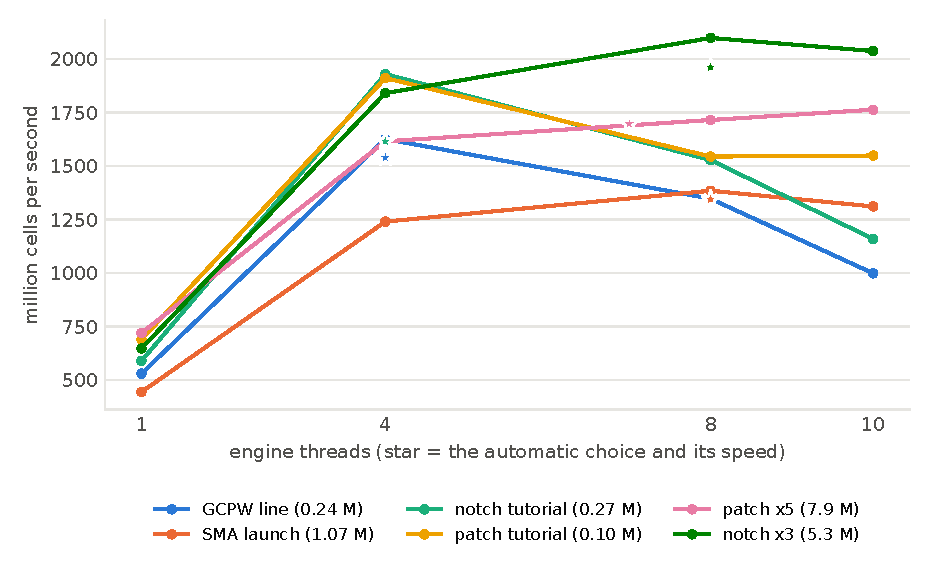
\includegraphics[width=0.85\textwidth]{fig_threads}
\caption{Thread scaling of snapshot cg14 (the check runs of 2026-10-29, \code{results/*\_cg14.txt}). Stars: the
automatic choice and the speed it reached, which includes the search of about 1.5\,s (project log; none for the patch
tutorial: its 0.7\,s run ends before the search prints its choice).}\label{fig:threads}
\end{figure}

\begin{table}[H]\centering\small
\begin{tabular}{@{}lrrrrrr@{}}
\toprule
model & stock (thr) & 1 thr & 4 thr & 8 thr & 10 thr & auto (picked) \\
\midrule
GCPW line (0.24\,M)      & 300 (4)  & 530 & 1627 & 1348 & 999  & 1540 (4) \\
SMA launch (1.07\,M)     & 437 (4)  & 444 & 1241 & 1385 & 1311 & 1344 (8) \\
notch tutorial (0.27\,M) & 318 (4)  & 590 & 1930 & 1528 & 1160 & 1615 (4) \\
patch tutorial (0.10\,M) & 277 (2)  & 690 & 1912 & 1545 & 1550 & 1499 (--) \\
patch x5 (7.9\,M)        & 1041 (8) & 720 & 1616 & 1716 & 1764 & 1697 (7) \\
notch x3 (5.3\,M)        & 845 (8)  & 648 & 1841 & 2099 & 2038 & 1962 (8) \\
\bottomrule
\end{tabular}
\caption{Snapshot cg14, \MC; fdtdKit columns from \code{results/*\_cg14.txt} (the run label in those files is
\code{cgy}). Stock: the best of the Table~\ref{tab:step1} sweep for the tutorials; for the two boards one 4-thread
reference run each (cg10 GCPW, cg14 SMA), as their stock thread count was not swept. The patch tutorial's 0.7\,s auto
run ends before the search prints its choice.}
\label{tab:final}
\end{table}

Two patterns of cg14 deserve a sentence. Single-thread speed rose 1.8 to 4.4 times over stock's sse-compressed engine
on the four models that have a stock single-thread run (Table~\ref{tab:step1}; the inner loop, the allocation
stagger, the boundary paths); of the patch tutorial's 2.7 times, the fork's base alone gives 1.18 times at one thread (296.6
against 251.3\,\MC, both with the multithreaded engine on one thread; \code{results/patch\_s1\_n10500\_base.txt}). And
the best thread count is 4 for models up to a few hundred thousand cells, where the four P cores saturate what the
per-step synchronisation leaves, and 8 to 10 above a million, where the E cores add bandwidth; the automatic choice
finds this within 3--7\,\% on the two boards and the two large models, while on the 0.6--2.7\,s tutorial runs the
search itself costs 16--22\,\% (in the cg18 check the GCPW line's 2.4\,s automatic run also lost 13\,\%). In cg29,
whose neighbour flags replace the two barriers per time step (Section~\ref{sec:cg29}), 8 threads was the fastest
setting measured on all six models, the smallest included (Section~\ref{sec:current}).

\subsection{The current build on the CPU and on the GPU (cg29)}\label{sec:current}
Table~\ref{tab:current} sets the current build, cg29 (patches 0001--0027), against stock v0.37.0 on the six models,
on the CPU and on the Metal diamond engine of Section~\ref{sec:gpu}, in one paired interleaved run per model on
2026-11-05 (\code{results/speed\_cg29\_2026-11-05.txt}; 4 rounds, the step counts of \code{bench/check.sh}). On the
CPU, cg29's best setting of the three measured (4 and 8 threads and the automatic count) is 8 threads on every
model, the patch tutorial's 0.104\,M cells included; the automatic count ran 1.2--7.5\,\% below it (the medians of
the rows). At 8 threads cg29 runs the four models of up to about a million cells at 1\,808--1\,961\,\MC,
4.73--6.89$\times$ stock at stock's best of 2, 4 and 8 threads, and the two large models at 1\,958 (patch x5) and
2\,177\,\MC\ (notch x3), 1.95$\times$ and 2.72$\times$. The Metal diamond engine runs the four at 4.83--7.40$\times$
stock and the two large models at 2.87$\times$ and 3.99$\times$. Against the CPU engine at its best, paired in the
same rounds, it is ahead on patch x5 (1.47$\times$), notch x3 (1.46$\times$) and the GCPW line (1.17$\times$), level
on the SMA launch (1.00$\times$; 0.99--1.13 over the rounds) and behind on the notch tutorial (0.97$\times$) and the
patch tutorial (0.93$\times$). Grid size decides most of this (Figure~\ref{fig:crossover}): in a sweep of three models
over 0.1--7.9\,M cells the GPU led in every round from 1.7--2.9\,M cells on and by 1.25--1.52$\times$ above 3\,M, and
below that the two engines were within 0.89--1.23$\times$ of each other, the side depending on the model and on the
session. On the patch tutorial, whose nf2ff dumps end a GPU call every 31 steps, the GPU stands idle for 18--27\,\% of the
time-stepping loop, while the CPU evaluates the dumps and while each call's command buffers start and finish; on the
notch tutorial it is busy 97\,\% of the time but runs slower on so small a grid
(Section~\ref{sec:gpu}).

Every CPU run's port probes are identical to stock's at 4 threads. The GPU runs differ from them by
$1.7\times10^{-7}$ to $9.4\times10^{-7}$ relative: Apple's GPU flushes subnormal numbers to zero and the CPU keeps
them, and with \code{OPENEMS\_FTZ=1} on the CPU the two engines are identical on all six models
(\code{results/*\_cg29gpu.txt}; Section~\ref{sec:policy}). The SMA launch runs here on the 1.071\,M-cell mesh of the
earlier tables (\code{RFSIM\_MIN\_CELL=0.02}), not on the 0.871\,M cells that the toolkit's default has built since
2026-11-04 (Table~\ref{tab:models}); rates on the two meshes do not compare. A round started once the other processes
were quiet and was run again (on the SMA launch, a single run) when they rose above the limit during it (the caption
gives the rule); during the runs kept the others used a median of 0.5--0.8 cores per model, at most 1.5.

Two things set Table~\ref{tab:current} apart from Table~\ref{tab:final}: its stock reference ran in the same rounds,
at 2, 4 and 8 threads on every model, while Table~\ref{tab:final} took stock's rates for the tutorials from the
step-1 sweep and one 4-thread run for each board; and its snapshot is cg29, not cg14. Stock's rates also differ
between the two sessions (the SMA launch at 4 threads 437 against 379\,\MC, both on the 1.071\,M mesh), so the ratio
of the two tables' factors is not cg29's gain over cg14. For cg29 against cg18, paired with each other in rounds of
their own over the six models (5 rounds, other processes on 0.3--0.6 cores, the SMA launch on its 0.871\,M mesh),
Section~\ref{sec:cg29} gives 1.03--1.23$\times$ at 4 threads and 1.13--1.44$\times$ at 8
(\code{results/cpu\_items\_cg29\_2026-11-05.txt}, section 4).

% Generated by figures/tables.py from results/speed_cg29_2026-11-05.txt; edit the script, not this file.
\begin{table}[H]\centering\small
\resizebox{\ifdim\width>\textwidth\textwidth\else\width\fi}{!}{\begin{tabular}{@{}lrrrrrrrr@{}}
\toprule
 & stock v0.37.0 & \multicolumn{3}{c}{cg29, CPU (multithreaded)} & cg29, GPU & \multicolumn{3}{c@{}}{paired ratio} \\
\cmidrule(lr){2-2}\cmidrule(lr){3-5}\cmidrule(lr){6-6}\cmidrule(l){7-9}
model (cells) & best (thr) & 4 thr & 8 thr & auto & diamond & CPU / stock & GPU / stock & GPU / CPU \\
\midrule
GCPW line (0.242\,M) & 286 (4) & 1548 & \textbf{1808} & 1689 & 2113 & 6.33 & 7.40 & 1.17 \\
SMA launch (1.071\,M) & 379 (4) & 1388 & \textbf{1833} & 1799 & 1829 & 4.73 & 4.83 & 1.00 \\
notch tutorial (0.270\,M) & 303 (4) & 1595 & \textbf{1961} & 1814 & 1893 & 6.56 & 6.26 & 0.97 \\
patch tutorial (0.104\,M) & 268 (2) & 1829 & \textbf{1854} & 1832 & 1729 & 6.89 & 6.48 & 0.93 \\
patch x5 (7.86\,M) & 1003 (8) & 1705 & \textbf{1958} & 1889 & 2879 & 1.95 & 2.87 & 1.47 \\
notch x3 (5.25\,M) & 800 (8) & 1736 & \textbf{2177} & 2097 & 3193 & 2.72 & 3.99 & 1.46 \\
\bottomrule
\end{tabular}}
\caption{Snapshot cg29 (patches 0001--0027) against stock v0.37.0 on the six models, \MC, measured on 2026-11-05 (\code{results/speed\_cg29\_2026-11-05.txt}). One paired interleaved run per model (\code{bench/abtest.py}, 4 rounds, the step counts of \code{bench/check.sh}): every round runs stock at 2, 4 and 8 threads, cg29's multithreaded engine at 4 and 8 threads and with the automatic thread count, and cg29's Metal diamond engine, in turn, once the other processes use at most 1.5 cores and 10\,\% of the GPU, and is run again, up to three times, when they rose above that during one of its runs; the SMA launch row comes from a re-run that repeats the single loaded runs instead (\code{--run-redo 3}). Rates: the median over the rounds; ratios: the median of the per-round ratios. Stock: the best of its three thread counts. Bold: cg29's best CPU setting, which the two CPU ratios use. Every CPU run's port probes are identical to stock's at 4 threads; the GPU runs differ from them by at most $9.4\times10^{-7}$ relative, because the GPU flushes subnormal numbers (with \code{OPENEMS\_FTZ=1} on the CPU they are identical, \code{results/*\_cg29gpu.txt}). The SMA launch on the 1.071\,M-cell mesh of the earlier tables (\code{RFSIM\_MIN\_CELL=0.02}); the toolkit's default since 2026-11-04 builds 0.871\,M cells. The other processes used a median of 0.5--0.8 cores per model during the runs kept.}\label{tab:current}
\end{table}


\subsection{End-to-end run time}
Figure~\ref{fig:runtime} and Table~\ref{tab:e2e} give the number the author cares about: the wall time of a complete
simulation of each board from the toolkit, timed around its \code{FDTD.Run} call (operator setup and time stepping).
All runs were made on 2026-11-03 with the toolkit as it was that day and the meshes it built, one per board with
stock v0.37.0 and one per setting with cg18 (\code{results/rfsim\_e2e\_2026-11-03.txt}). The columns are:
the full run with stock, which goes to \code{max\_time} because the energy criterion never fires
(Section~\ref{sec:probeend}); the same full run with fdtdKit, same steps, so the difference is the solver's alone;
fdtdKit with the probe end at $-60$\,dB and a hold of 1, the toolkit's default until 2026-11-04; and a hold of 0.5
with, on the SMA launch, the 0.05\,mm mesh floor of
Section~\ref{sec:meshfloor}, the shortest setting tested, which the author made the toolkit's default on 2026-11-04
(toolkit commit 4a7e20e). Model and Gaussian pulse are
the same in every column (the SMA launch's mesh is coarser in the last). The solver alone gives 5.6$\times$ on the
GCPW line and 3.3$\times$ on the SMA launch; the probe end with the earlier defaults brings this to 8.9$\times$ and
5.8$\times$, the toolkit's current defaults to 14.7$\times$ and 15.0$\times$, at the accuracy costs of
Tables~\ref{tab:probeend} and~\ref{tab:mesh}. Stock ran with the thread counts the toolkit uses
for a stock library, 4 on the GCPW line and 8 on the SMA launch, the same counts the tuner picked for the two full
runs. On the SMA launch this 8-thread stock run reached 348\,\MC, while stock's 4-thread bench run on the same board
reached 437\,\MC\ (Table~\ref{tab:final}): the SMA factors are against the toolkit's stock setting.

\begin{figure}[htbp]\centering
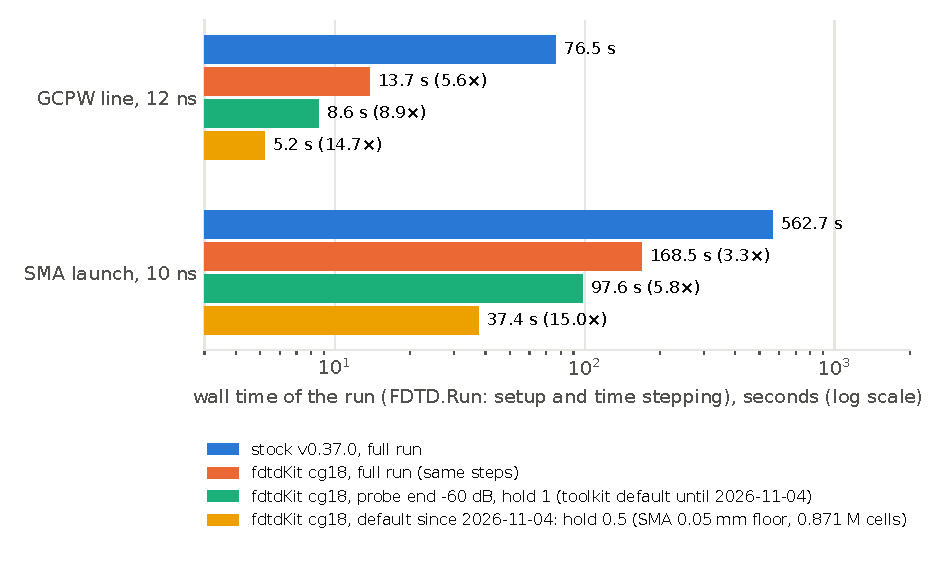
\includegraphics[width=0.85\textwidth]{fig_runtime}
\caption{Wall time of \code{FDTD.Run} for a complete simulation of the two boards, measured on 2026-11-03
(Table~\ref{tab:e2e}): stock v0.37.0 and fdtdKit (snapshot cg18) for the full run, cg18 with the probe end at
$-60$\,dB and a hold of 1 (the toolkit's default until 2026-11-04), and
cg18 with the toolkit's defaults since 2026-11-04 (a hold of 0.5; on the SMA launch also the 0.05\,mm mesh floor).
Labels: the time and, for fdtdKit, the factor against stock.}\label{fig:runtime}
\end{figure}

\begin{table}[H]\centering\small
\resizebox{\ifdim\width>\textwidth\textwidth\else\width\fi}{!}{\begin{tabular}{@{}lrrrrr@{}}
\toprule
 & & stock v0.37.0 & \multicolumn{3}{c@{}}{fdtdKit (cg18)} \\
\cmidrule(lr){3-3}\cmidrule(l){4-6}
 & & full run & full run & probe end $-60$\,dB, & toolkit default \\
board & cells & & (same steps) & hold 1$^{\dagger}$ & since 2026-11-04$^{*}$ \\
\midrule
GCPW line, 50\,mm, 12\,ns & 0.242\,M & 94\,217 steps & 94\,217 steps & 45\,570 steps & 34\,300 steps \\
 & & 76.5\,s & 13.7\,s, 5.6$\times$ & 8.6\,s, 8.9$\times$ & 5.2\,s, 14.7$\times$ \\
\addlinespace
SMA launch, 10\,ns & 1.071\,M & 182\,622 steps & 182\,622 steps & 103\,831 steps & 50\,320 steps \\
 & & 562.7\,s & 168.5\,s, 3.3$\times$ & 97.6\,s, 5.8$\times$ & 37.4\,s, 15.0$\times$ \\
\bottomrule
\end{tabular}}
\caption{End-to-end runs of the two boards from the author's toolkit, measured on 2026-11-03 with snapshot cg18
(patches 0001--0006, the build installed on the author's Mac from 2026-11-04 to 2026-11-06) and with stock v0.37.0,
one run each on a quiet
machine (before each run the other
processes used less than one core for 10\,s; the file gives their load during each run), all on meshes that the
toolkit built that day (\code{results/rfsim\_e2e\_2026-11-03.txt}). Time: wall time of \code{FDTD.Run}
(operator setup and time stepping); the model build (0.11--0.79\,s) and the port evaluation (\code{CalcPort}, at most
0.03\,s) are not included. Factor: stock time over fdtdKit time. Stock ran with the thread counts the toolkit uses for
a stock library (4 on the GCPW line, 8 on the SMA launch), fdtdKit with its tuner; the stock full runs' port files are
byte-identical to fdtdKit's. In the GCPW's $-60$\,dB, hold 1 run the tuner picked 8 threads (1\,304\,\MC, against
1\,636--1\,683\,\MC\ at 4 threads in the other fdtdKit GCPW runs). $^{\dagger}$The toolkit's default until
2026-11-04. $^{*}$Probe end $-60$\,dB with a hold of
0.5; on the SMA launch also the 0.05\,mm mesh floor of Section~\ref{sec:meshfloor} (0.871\,M cells); the GCPW line
has no mesh floor. The shortest setting tested on 2026-11-03; the author made it the toolkit's default on 2026-11-04
(toolkit commit 4a7e20e).}\label{tab:e2e}
\end{table}

Table~\ref{tab:e2ecg29} has the same boards with cg29 on 2026-11-05, with the toolkit's current defaults and as full
runs (the SMA launch on its 0.871\,M mesh in both), on the CPU (the multithreaded engine with the automatic thread
count) and on the Metal diamond engine, in interleaved rounds (\code{results/rfsim\_e2e\_cg29\_2026-11-05.txt}).
Paired per round, the GPU ran the default runs
1.37$\times$ (GCPW line) and 1.22$\times$ (SMA launch) as fast as the CPU engine and both full runs 1.17$\times$; over
the rounds in which both runs were clean the ratios were 1.27$\times$ and 1.21$\times$ for the default runs (two
rounds each) and 1.23$\times$ and 1.08$\times$ for the full runs (one round each). Both engines stopped at the same
steps, and the GPU's results differ from the CPU's by the amounts in the caption, as the GPU flushes subnormal
numbers and the CPU runs here keep them. These runs saw more load than those of Table~\ref{tab:e2e}: the other
processes used a median of 1.0--1.6 cores per row, and in 5 of the 20 runs kept they stayed above the limit through
the third redo. In the one round in which both of the SMA launch's default runs were loaded, the CPU took 36.2\,s
against 27.9--28.9\,s in the clean rounds and the GPU 24.4\,s against 23.5--23.6\,s. With that load the CPU
columns are not a comparison with cg18: the GCPW line's default run took 5.6\,s on cg29's CPU engine here and 5.2\,s
on cg18's quiet run of Table~\ref{tab:e2e}, while in bench runs that pair the two builds round by round (5 rounds,
other processes on 0.4 cores) cg29's automatic thread count runs that board 1.30$\times$ and the SMA launch, on the
same 0.871\,M mesh, 1.42$\times$ as fast as cg18's (\code{results/cpu\_items\_cg29\_2026-11-05.txt}, section 4).
Since 2026-11-06 cg29 is the installed build (Section~\ref{sec:method}), so the toolkit's runs, on the CPU engine with
the automatic thread count and the probe end, run on it with no change on the toolkit's side; the Metal engine stays
opt-in, and the toolkit does not select it.

% Generated by figures/tables.py from results/rfsim_e2e_cg29_2026-11-05.txt; edit the script, not this file.
\begin{table}[H]\centering\small
\resizebox{\ifdim\width>\textwidth\textwidth\else\width\fi}{!}{\begin{tabular}{@{}lrrrrrrr@{}}
\toprule
 & & & \multicolumn{3}{c}{cg29, \code{FDTD.Run} wall time} & \multicolumn{2}{c@{}}{2026-11-03, same steps} \\
\cmidrule(lr){4-6}\cmidrule(l){7-8}
run & cells & steps & CPU & GPU & CPU / GPU & stock & cg18 \\
\midrule
GCPW line, full run & 0.242\,M & 94\,217 & 13.1\,s & 11.2\,s & 1.17$\times$ & 76.5\,s & 13.7\,s \\
GCPW line, toolkit default & 0.242\,M & 34\,300 & 5.6\,s & 4.1\,s & 1.37$\times$ & -- & 5.2\,s \\
SMA launch, full run & 0.871\,M & 118\,475 & 68.1\,s & 58.5\,s & 1.17$\times$ & -- & -- \\
SMA launch, toolkit default & 0.871\,M & 50\,320 & 28.9\,s & 23.6\,s & 1.22$\times$ & -- & 37.4\,s \\
\bottomrule
\end{tabular}}
\caption{End-to-end runs of the two boards from the author's toolkit with snapshot cg29 on 2026-11-05 (\code{results/rfsim\_e2e\_cg29\_2026-11-05.txt}): the multithreaded engine with the automatic thread count (CPU) against the Metal diamond engine (GPU), with the toolkit's defaults since 2026-11-04 (SMA mesh floor 0.05\,mm, 0.871\,M cells; probe end $-60$\,dB with a hold of 0.5 excitation lengths: ``toolkit default'') and with the probe end off (``full run'', to \code{max\_time}: GCPW 12\,ns, SMA 10\,ns). Time: wall time of \code{FDTD.Run} (operator setup and time stepping), the median over 2--3 interleaved rounds; each run started once the other processes used at most 1.5 cores and 10\,\% of the GPU and was run again, up to three times, when they rose above that during it; in 5 of the 20 runs kept the others stayed above that through the third redo (at most 4.4 cores): the medians include them, and the file gives the medians of the clean runs as well. CPU\,/\,GPU: the median of the per-round ratios of the run times. In every round both engines stop at the same step; the GPU's results differ from the CPU's by at most $7.3\times10^{-3}$\,dB in $S_{11}$ (where $|S_{11}|>-40$\,dB), $2.0\times10^{-4}$\,dB in $S_{21}$ and $5.4\times10^{-3}$\,$\Omega$ in $Z_0$ at the reference frequency, as the GPU flushes subnormal numbers (the file gives each round). The last two columns are the runs with the same settings and steps in Table~\ref{tab:e2e} (one run each, stock with the toolkit's 4 threads, cg18 with its tuner, on a quiet Mac: the others below one core for 10\,s before each run); the SMA's full run on the 0.871\,M mesh was not made there. During the runs here the others used a median of 1.0--1.6 cores per row, so the CPU columns are not a comparison with cg18 (paired, cg29 against cg18: Section~\ref{sec:cg29}).}\label{tab:e2ecg29}
\end{table}


\subsection{Common benchmarks}\label{sec:common}
The tables so far use this project's own models. Four measurements of 2026-11-10 use tests that readers outside the
project know by name: upstream's own benchmark on current master, STREAM, a free-space cube after the gprMax benchmark
models, and the radar cross-section of a metal sphere against the Mie series
(\code{results/common\_benchmarks\_2026-11-10.txt}; \code{scripts/common\_bench/}). The fork is the installed build
cg29 in all four.

\paragraph{Upstream's benchmark, and master's new engine.}
Upstream master has a benchmark tool, \code{benchmark/bench.py}: six cases (an empty box, a box with PML, an
inhomogeneous one, a dispersive one, an antenna with field dumps, a cylindrical mesh) at about 1\,M (size S) and
8\,M cells (size M), each timed for 3\,s of time stepping with the \code{openEMS} binary. Since the fork's base,
master has also gained a third engine, \code{--engine=cpu}, beside \code{multithreaded} and
\code{gpu}~\cite{thliebig495}. The tool ran twice on master 1d710c2: master alone on its three engines (part A), and
master against the fork on the \code{multithreaded} engine, the one engine both have, interleaved as upstream asks
(part B); 4 and 8 threads, three repeats (Table~\ref{tab:upstream}). During both parts the other processes used a
median of 0.22 cores (three of 75 samples above 0.8). The tool's column that says whether two builds compute the same
thing was not produced: it needs master's Python module, which was not built.

\begin{table}[H]\centering\small
\begin{tabular}{@{}llrrrrrr@{}}
\toprule
 & & \multicolumn{3}{c}{part B, interleaved} & \multicolumn{3}{c@{}}{part A, master alone} \\
\cmidrule(lr){3-5}\cmidrule(l){6-8}
case & size & master & fdtdKit & ratio & master & master & master \\
 & & \code{multithr.} & \code{multithr.} & & \code{multithr.} & \code{cpu} & \code{gpu} \\
\midrule
ideal & S & 1\,181 & 2\,456 & 2.08$\times$ & 1\,267 & 1\,907 & 1\,703 \\
pml & S & 189 & 1\,056 & 5.60$\times$ & 201 & 709 & 1\,163 \\
inhomogeneous & S & 187 & 1\,014 & 5.42$\times$ & 203 & 678 & 1\,153 \\
dispersive & S & 48 & 479 & 10.0$\times$ & 53 & 921 & 737 \\
antenna & S & 148 & 871 & 5.87$\times$ & 162 & 679 & 1\,078 \\
cylindrical & S & 911 & 1\,544 & 1.69$\times$ & 1\,029 & 1\,304 & 1\,537 \\
\addlinespace
ideal & M & 1\,088 & 1\,739 & 1.60$\times$ & 1\,360 & 2\,099 & 1\,689 \\
pml & M & 277 & 1\,061 & 3.83$\times$ & 295 & 1\,225 & 1\,414 \\
inhomogeneous & M & 266 & 967 & 3.63$\times$ & 286 & 1\,188 & 1\,413 \\
dispersive & M & 53 & 448 & 8.47$\times$ & 52 & 1\,109 & 739 \\
antenna & M & 214 & 908 & 4.24$\times$ & 230 & 1\,088 & 1\,334 \\
cylindrical & M & 823 & 1\,012 & 1.23$\times$ & 921 & 1\,755 & 1\,590 \\
\bottomrule
\end{tabular}
\caption{Upstream's \code{benchmark/bench.py} on the M5, 2026-11-10, in \MC: the better of 4 and 8 threads per
cell of the table, each the median of three repeats as the tool reports it. Master: openEMS 1d710c2 with CSXCAD
fdff4b5; fdtdKit: the installed cg29. Part B ran the two builds interleaved; part A ran master alone, 15 minutes
earlier, so its \code{cpu} and \code{gpu} columns are not paired with the fork. The tool's spread was below 5\,\%
in most rows and above 10\,\% in ten of the 120 (master's dispersive S rows in part B, 23 and 26\,\%, among
them); the file has every row.}\label{tab:upstream}
\end{table}

On the engine both builds have, the fork runs 1.23--8.5$\times$ as fast as master at 8\,M cells and
1.69--10.0$\times$ at 1\,M, the least on the cylindrical mesh and the most on the dispersive case, as against v0.37.0
(Section~\ref{sec:cg29}). Master's new \code{cpu} engine changes the picture at 8\,M cells: taken as measured,
its rates are 1.15--1.23$\times$ the fork's on the ideal, pml, inhomogeneous and antenna cases, 1.73$\times$ on the
cylindrical mesh and 2.5$\times$ on the dispersive case. The two columns come from different parts, and master's own
\code{multithreaded} rates were 6--25\,\% higher in part A than in part B (dispersive M: 2\,\% lower); with each engine
taken relative to master's \code{multithreaded} rate of its own part, the \code{cpu} engine is level with the fork
on the ideal case (0.97$\times$), 1.08--1.14$\times$ on pml, inhomogeneous and antenna, 1.55$\times$ on the
cylindrical mesh and 2.5$\times$ on the dispersive case. At 1\,M cells the fork is ahead of the \code{cpu} engine on
five cases (1.18--1.50$\times$ as measured) and behind on the dispersive one (0.52$\times$). So on large grids
upstream's own new engine is level with or ahead of this fork's CPU engine, and well ahead with dispersive material;
a paired run of the two, with the probes compared, has not been made. The fork's Metal diamond engine was not part of
this run: every case of the tool uses the steady-state detection, which that engine runs on its CPU loops
(Section~\ref{sec:future}).

\paragraph{STREAM.}
The introduction takes the machine's memory bus as about 150\,GB/s from Apple's figure. STREAM~\cite{stream}, the
usual measure of sustained memory bandwidth (version 5.10, 100\,M elements per array, OpenMP, the best of 20 passes),
gives Table~\ref{tab:stream}: 120--130\,GB/s at 4 threads and 125--138\,GB/s at 8 and 10, and one thread alone
already draws 110--115\,GB/s. STREAM counts 16 or 24 bytes per element and not the read that a store to a new cache
line may cost, so its figures are a lower bound of the traffic. They sit where this paper's kernels do: the Metal
kernels drew 121--127\,GB/s (Section~\ref{sec:gpu}), and the fused CPU sweep 95\,GB/s at 4 threads
(Section~\ref{sec:engine}). A system process held one core during the run.

\begin{table}[H]\centering\small
\begin{tabular}{@{}lrrrr@{}}
\toprule
threads & Copy & Scale & Add & Triad \\
\midrule
1 & 114.3 & 110.4 & 114.5 & 115.3 \\
4 & 129.0 & 130.3 & 120.3 & 120.1 \\
8 & 135.9 & 125.5 & 124.7 & 125.0 \\
10 & 137.7 & 125.7 & 126.2 & 126.1 \\
\bottomrule
\end{tabular}
\caption{STREAM 5.10 on the M5 (16\,GB), best rate in GB/s ($10^9$ bytes per second), 2026-11-10; Apple clang
\code{-O3 -mcpu=native}, OpenMP, 100\,M elements per array.}\label{tab:stream}
\end{table}

\paragraph{A free-space cube.}
The gprMax project times its solver on cubes of free space with one dipole source and its default 10-cell
absorbing boundary, from $100^3$ to $800^3$ cells~\cite{gprmax,gprmaxgpu}. The model \code{cube} of
\code{bench/models.py} builds the same problem in openEMS: $N^3$ cells of 1\,mm, one excited cell edge at the
centre, \code{PML\_10} on all six faces, one voltage probe. Table~\ref{tab:cube} has $N=100$ to 400, the largest
that 16\,GB hold with room to spare, in three paired rounds per size. These are rates of one model on three builds of
one solver; they are not set against the rates that gprMax publishes for its own code.

\begin{table}[H]\centering\small
\begin{tabular}{@{}rrrrrrrrr@{}}
\toprule
$N$ & cells & steps & stock & fdtdKit & fdtdKit & Metal & CPU / & Metal / \\
 & & & best & 4 thr & 8 thr & diamond & stock & CPU \\
\midrule
100 & 1.0\,M & 6\,000 & 181 & 923 & 1\,222 & 992 & 6.77$\times$ & 0.81$\times$ \\
150 & 3.4\,M & 1\,800 & 256 & 1\,038 & 1\,339 & 1\,353 & 5.22$\times$ & 1.01$\times$ \\
200 & 8.0\,M & 800 & 299 & 1\,030 & 1\,228 & 1\,470 & 4.11$\times$ & 1.20$\times$ \\
300 & 27\,M & 600 & 370 & 946 & 1\,097 & 1\,703 & 2.97$\times$ & 1.55$\times$ \\
400 & 64\,M & 600 & 439 & 875 & 1\,034 & 1\,834 & 2.35$\times$ & 1.77$\times$ \\
\bottomrule
\end{tabular}
\caption{The free-space cube with a 10-cell PML on every face, 2026-11-10, in \MC: medians of three paired rounds
(\code{bench/abtest.py}). Stock: v0.37.0 at the better of 4 and 8 threads ($N\ge300$: 8 threads only); fdtdKit:
cg29, \code{multithreaded}. Ratios: of the medians, the CPU ratio with fdtdKit at 8 threads. Every CPU run's probe is
identical to stock's; the Metal engine's differs by $5.9\times10^{-7}$ to $3.9\times10^{-6}$ relative (it flushes
subnormals). Other processes: a median of 1.3--1.6 cores during the runs of $N=100$ and 150, where a run that saw
them above the limit of 1.5 cores was kept after one redo in every round, and 0.3--0.7 cores for
$N\ge200$, where that happened in one round each at $N=200$ and 300.}\label{tab:cube}
\end{table}

The absorbing boundary sets the scale of these rates. At $N=100$ the six PML slabs hold 49\,\% of the cells and at
$N=400$ 14\,\%, and stock updates PML cells far more slowly than plain ones, so stock's rate rises from 181 to
439\,\MC\ with the size, the opposite of the six models. The fork's CPU engine stays at 1\,034--1\,339\,\MC, 2.4 to
6.8 times stock. The Metal diamond engine passes the CPU engine at about 3\,M cells, as in
Figure~\ref{fig:crossover}, and at 64\,M cells it runs 1.77$\times$ as fast, the largest lead in a paired run of
this project; its rate still rises at the largest size.

\paragraph{A metal sphere against the Mie series.}
The monostatic radar cross-section of a perfectly conducting sphere has an exact series
solution~\cite{mie}, and openEMS ships the case as a tutorial (\code{RCS\_Sphere}: radius 200\,mm, a plane wave from
a total-field/scattered-field box, \code{PML\_8}, the far field through the nf2ff box).
\code{scripts/common\_bench/mie.py} runs it with a fixed number of steps and compares 95 frequencies, $ka=0.41$ to
4.19, with the series (Table~\ref{tab:mie}).

\begin{table}[H]\centering\small
\begin{tabular}{@{}llrrr@{}}
\toprule
cell at 1\,GHz & build, engine & cells & mean $|$error$|$ & largest \\
\midrule
$\lambda/20$ (the tutorial's) & stock v0.37.0 & 0.57\,M & 0.770\,dB & 2.943\,dB \\
$\lambda/20$ & fdtdKit, multithreaded & 0.57\,M & 0.770\,dB & 2.943\,dB \\
$\lambda/40$ & fdtdKit, multithreaded & 4.33\,M & 0.357\,dB & 0.880\,dB \\
$\lambda/40$ & fdtdKit, Metal diamond$^{*}$ & 4.33\,M & 0.357\,dB & 0.880\,dB \\
\bottomrule
\end{tabular}
\caption{Backscatter of a PEC sphere of 200\,mm radius against the Mie series, 95 frequencies with $ka$ from 0.41
to 4.19, 2026-11-10; 1\,400 steps at $\lambda/20$ and 2\,000 at $\lambda/40$. $^{*}$The engine has no GPU version of
the plane-wave source and ran its CPU loops.}\label{tab:mie}
\end{table}

The error is the method's and the mesh's: a staircased sphere on a uniform mesh, with a mean that halves when the cell is halved.
It is not the fork's. Stock and fork give the same error to the digits shown; their cross-sections differ by at most
$2.5\times10^{-6}$ relative, all of it from the fork's separable far-field routine
(Section~\ref{sec:beyond}), and with that routine switched off (\code{OPENEMS\_NF2FF\_LEGACY=1}) the two are identical
at all 100 frequencies. One thing this case showed about the tutorial itself: with its energy end criterion the stop
step is not reproducible (1\,104 and 1\,340 steps in two stock runs), because the engine tests the criterion between
chunks of steps whose length follows the measured speed, and two such runs differ by up to $1.6\times10^{-3}$ in
the cross-section. Comparisons across builds need a fixed step count, as everywhere else in this paper.

\section{After publication: the build of 2026-11-11 (cg31)}\label{sec:cg31}

Every table before this section is of snapshot cg29 or earlier. On 2026-11-11, the day after the repository was
published, twelve commits followed (patches 0028 to 0039): one on the energy schedule of a run without an end criteria
(0028), ten on the Metal diamond engine (0029 to 0038) and one on the cylinder extension (0039). The build, cg31, has
been the installed one on the author's Mac since that day. This section records what was looked for, what changed and
what it gave (\code{results/metal\_engine\_cg31\_2026-11-11.txt}).

\subsection{Where the Metal engine's time went}
Three observations set the work list.

\emph{An energy sum on one thread.} The fork's base estimates the field energy every Nyquist period during the first
60\,s of a run, so that a run with an end criteria stops at a reproducible step. The estimate is one pass of one CPU
thread over both fields, and the engine waits for it. On a benchmark model with a Nyquist period of 51 steps this was
4--6\,\% of the time-stepping loop on 3--17\,M cells; with a period of 519 steps the time lost outside the engine fell
from 0.23\,s to 0.03\,s per 3\,000 steps (project log). A run with a fixed number of steps and no end criteria has
nothing to stop on, so it now makes no such estimates (patch 0028), as in v0.37.0. The author's board runs have a
criteria and Nyquist periods above a thousand steps: for them the estimate costs 0.1--0.2\,\% (project log) and stays.

\emph{Extensions cost by being present.} In a timing-only build that leaves parts of the kernel out (results wrong by
design), the GCPW line ran 1.35$\times$ as fast without its Mur faces, 1.32$\times$ without its conducting sheets and
2.0$\times$ without any extension; the SMA launch 1.69$\times$ without its UPML slab on one z face.
But on a later snapshot, where the same builds of the GCPW line gave 1.26$\times$, 1.22$\times$ and 1.94$\times$,
skipping one stage at run time, with the code still in the kernel, gave only 1.02--1.07$\times$ each (the sheets' Pre
and Apply, Mur's Pre and Post). The cost is tied to the code being compiled into the kernel, not
to the loops over the few cells it handles; what in the GPU's execution makes it so was not found. Empty extra barriers
cost nothing measurable, and moving the Pre stages of Mur and of the sheets into the half-step before, beside the cell
update, which saves one barrier per half-step with identical fields, ran 2--4\,\% \emph{slower} and was dropped.

\emph{Not at the bus on mid-size grids.} Counted from the tile schedule, a tile that stays cached for its block loads
and stores 20--29 bytes of field per cell and time step, which at the measured rates is 79--105\,GB/s at 3\,M cells,
below the 125--138\,GB/s that STREAM measures on this machine (Section~\ref{sec:common}); the count assumes perfect
reuse within a block and was not measured. At 17\,M cells with 257 z lines a tile is 0.9--1.5\,MB, because a tile
holds every z line, and the shallower $K=3$ tilings win although they move more bytes (the byte counts and tile sizes
of this paragraph are from the project log).

\subsection{What changed}
\begin{table}[H]\centering\small
\begin{tabular}{@{}lp{0.60\textwidth}l@{}}
\toprule
patch & change & switch (default on) \\
\midrule
0028 & no energy schedule in a run without an end criteria & \\
0029, 0032 & Mur faces of one axis share a barrier; Post and Apply in one pass where a tile's faces are on one axis &
  \code{DIAMOND\_MURMERGE} \\
0029 & a call's rest in blocks of nearly equal depth (10 steps at $K=4$: 4, 3, 3) & \code{DIAMOND\_EVEN} \\
0030 & three dispatches per block: the mountain$\times$valley and valley$\times$mountain tiles do not depend on each
  other and go together & \code{DIAMOND\_MERGE} \\
0031, 0032, 0034 & no divergent branch for the z neighbour; divisions by run-time widths as multiplications by
  reciprocals from the host; threads without work leave a Mur stage early & \code{DIAMOND\_FASTIDX} \\
0031 & the pipeline is told that a threadgroup is a whole number of SIMD groups & \code{DIAMOND\_TGFLAG} \\
0033 & UPML of the boxes with every z line (the x and y slabs) a z-vector at a time & \code{DIAMOND\_PML4} \\
0035 & UPML of the z slabs three components of a cell at a time & \code{DIAMOND\_PML3} \\
0036 & dispersive materials (sheets, Drude/Lorentz, Debye) three components of a cell at a time & \\
0037 & offsets and counts of the extension data as constants of the kernel, which is compiled after the data are
  packed & \\
0038 & seven tilings in a two-stage tuner (adds $K=4$ with 10,6 and 9,2 tiles and $K=5$ with 12,8); the per-tile
  lists in their own buffer & \code{DIAMOND\_CAND} \\
0039 & line hooks for the cylinder extension (Section~\ref{sec:cg31cyl}) & \\
\bottomrule
\end{tabular}
\caption{The commits of 2026-11-11. Switch names carry the prefix \code{OPENEMS\_}; \code{=0} restores the earlier
behaviour (\code{DIAMOND\_CAND=4}: the four tilings of patch 0016). Every step was a snapshot of its own (cg30a to
cg30l, cg31a) that passed \code{scripts/checks/diamond\_check.sh} with 72 of 72 comparisons
identical.}\label{tab:cg31items}
\end{table}

The mountain$\times$valley and the valley$\times$mountain tiles of a block can share a dispatch because a mountain
cell reads only cells that were mountain cells one half-step earlier, in both directions: a cell leaves its x mountain
or its y mountain first, so it is updated by one of the two kinds only, and neither kind reads what the other writes
within the block. The UPML stages were scalar loops over single floats, three components and up to four lanes apart;
an x or y slab has every z line, so its cells fill whole z-vectors and one pass can update a float4 of one component
with the same operations per lane, while a z slab has one lane of a z-vector per cell and its pass now takes the
three components of a cell together. One build in this series was wrong: it computed the reciprocals for the
divisions on the GPU, and on this M5 (macOS 27.0.1) the GPU's own \code{0xffffffff / w} returns 3\,579\,139\,454 for
$w=3$, where 1\,431\,655\,765 is right. The identity check caught it as wrong fields on the Mur cases; the
reciprocals now come from the host.

\subsection{What it gave}
\begin{table}[H]\centering\small
\begin{tabular}{@{}lrrrrrr@{}}
\toprule
 & \multicolumn{3}{c}{Metal diamond engine} & \multicolumn{2}{c}{CPU engine, cg31} & Metal / \\
\cmidrule(lr){2-4}\cmidrule(lr){5-6}
model & cg29 & cg31 & cg31 / cg29 & 8 threads & 4 threads & CPU best \\
\midrule
GCPW line, 0.24\,M & 2\,118 & 2\,307 & 1.09$\times$ & 2\,000 & 1\,816 & 1.15$\times$ \\
SMA launch, 0.87\,M & 1\,854 & 2\,108 & 1.14$\times$ & 1\,955 & 1\,509 & 1.08$\times$ \\
patch tutorial, 0.10\,M & 1\,753 & 1\,887 & 1.08$\times$ & 1\,910 & 1\,868 & 0.99$\times$ \\
notch tutorial, 0.27\,M & 1\,904 & 2\,907 & 1.53$\times$ & 2\,129 & 1\,909 & 1.37$\times$ \\
patch x5, 7.86\,M & 2\,901 & 3\,100 & 1.07$\times$ & 2\,104 & 1\,802 & 1.47$\times$ \\
notch x3, 5.25\,M & 3\,210 & 3\,702 & 1.15$\times$ & 2\,330 & 1\,853 & 1.59$\times$ \\
\addlinespace
PEC box, 3.0\,M & 3\,692 & 4\,408 & 1.19$\times$ & 2\,614 & 2\,156 & 1.69$\times$ \\
PEC box, 17\,M & 3\,056 & 3\,507 & 1.15$\times$ & 1\,736 & 1\,550 & 2.02$\times$ \\
cube with 10-cell PML, 1.0\,M & 980 & 1\,546 & 1.58$\times$ & 1\,343 & 1\,012 & 1.15$\times$ \\
cube with 10-cell PML, 8.0\,M & 1\,483 & 1\,839 & 1.24$\times$ & 1\,293 & 1\,049 & 1.42$\times$ \\
\bottomrule
\end{tabular}
\caption{The Metal diamond engine before (cg29) and after (cg31) the commits of 2026-11-11, with cg31's CPU engine
beside it: median \MC\ of four paired rounds per model on 2026-11-11 with the other sessions on the machine paused
(the other processes used 0.2--0.9 cores; a run that saw more than 1.5 cores was repeated once). cg31 / cg29: the
median of the per-round ratios, which over the rounds stayed within 3\,\% of the value shown except on the patch
tutorial (0.92--1.13), the notch tutorial (1.42--1.53) and the two cubes (1.51--1.58 and 1.20--1.29). The PEC box is
the benchmark model of luikore's engine (Table~\ref{tab:threebuilds}), the cube that of Table~\ref{tab:cube}. The SMA
launch is on the toolkit's current mesh. Every cg31 Metal run's probes are identical to cg29's.}\label{tab:cg31}
\end{table}

The two boards gain 9 and 14\,\%; the notch tutorial and the PML cube gain the most (53\,\%, and 58 and 24\,\%), in
good part from the UPML stages on whole faces (patch 0033); the two large tutorial models gain 7 and 15\,\% and the
PEC box 19 and 15\,\%. With that the Metal engine is ahead of the CPU
engine on every model but the patch tutorial, where the two are level. cg31 also passed, on the CPU side,
\code{emskit fdtd check} on the six models against stock (all identical, 18 of 18 rows), the Debye check and both
boards end to end, which stop at the same steps as with cg29 (34\,300 and 50\,320); the validation suite on the Metal
engine (15 of 15) ran on the snapshot of patches 0001--0038 (cg30l), before the cylinder patch.

\subsection{Three builds on one model}\label{sec:threebuilds}
Section~\ref{sec:gpu} had no head-to-head with luikore's Metal engine~\cite{luikore228}: its diamond path refuses the
six models. It does run its own benchmark model, a uniform grid with PEC walls, one dielectric box and a point
excitation, so the three builds were run on that model, each binary from the same model file, interleaved, with the
other sessions paused (Table~\ref{tab:threebuilds}; \code{scripts/luikore\_compare/},
\code{results/engines\_on\_luikore\_model\_2026-11-11.txt}).

\begin{table}[H]\centering\small
\begin{tabular}{@{}lrr@{}}
\toprule
engine & 3.0\,M cells & 17.0\,M cells \\
\midrule
fdtdKit (cg31), Metal diamond & 3\,981 & 3\,309 \\
luikore PR \#228 (55ce11b), Metal & 3\,952 & 2\,829 \\
master 1d710c2, \code{gpu} & 1\,638 & 1\,566 \\
master 1d710c2, \code{cpu}, 8 threads & 1\,872 & 1\,933 \\
fdtdKit (cg31), \code{multithreaded}, best of 8 and 10 threads & 2\,371 & 1\,659 \\
luikore PR \#228, \code{multithreaded}, 8 threads & 1\,296 & 1\,042 \\
master 1d710c2, \code{multithreaded}, 8 threads & 1\,246 & 1\,055 \\
\bottomrule
\end{tabular}
\caption{Three builds on the benchmark model of luikore's engine, one Apple M5, 2026-11-11: median \MC\ of three
interleaved repetitions (3\,000 steps at 3.0\,M cells, 1\,000 at 17.0\,M); the other processes used a median of 0.44
cores before a run, at most 1.14. The \code{multithreaded} engines of the three builds give identical probes; the
others differ from them by $7\times10^{-6}$ to $3\times10^{-5}$ relative.}\label{tab:threebuilds}
\end{table}

On its own model luikore's engine and cg31's are level at 3.0\,M cells (1.01$\times$) and cg31's is 1.17$\times$ as
fast at 17\,M; the night before, cg29's had run 3\,728 and 3\,092, 0.94$\times$ and 1.09$\times$ luikore's in that
run (3\,958 and 2\,848; \code{results/luikore\_compare\_cg29\_2026-11-11.txt}). cg31's engine is 2.4$\times$ and
2.1$\times$ master's \code{gpu} engine here, luikore's 2.4$\times$ and 1.8$\times$.
On the CPU, cg31 is 1.27$\times$ master's new \code{cpu} engine at 3.0\,M cells and 0.86$\times$ at 17\,M: on the large
grid master's engine is ahead, as in Table~\ref{tab:upstream}. Two things qualify the table. It is one model, the best
case of a GPU engine (a regular grid, no boundary work). And a model file whose \code{endCriteria} is 0 makes the
\code{openEMS} program use its default of $-60$\,dB, so here the fork and master make the energy estimates of
Section~\ref{sec:cg31} and luikore's build does not: run from Python, where 0 means no criteria, cg31's Metal engine
does 4\,408 and 3\,507\,\MC\ on this model (Table~\ref{tab:cg31}).

Master's \code{cpu} engine blocks in time: all threads work in one tile of the size of the performance cores' cache
for up to eight steps. With that switched off (\code{OPENEMS\_CPU\_TBLOCK=0}) it ran upstream's ideal case at 8\,M
cells at 1\,347 and 1\,436\,\MC\ (4 and 8 threads) against 2\,010 and 2\,099 blocked the day before, and the PML case
at 891 and 1\,069 against 1\,117 and 1\,225: the blocking is worth 1.46--1.49$\times$ and 1.15--1.25$\times$ on this
machine (two runs a day apart). The fork's fused sweep, at 1\,739 on the ideal case, is ahead of master's unblocked
kernel and behind its blocked one. The experiment of Section~\ref{sec:rejected} that found no gain in temporal blocking
on the CPU gave every thread a sub-grid of its own, which does not fit the cache four threads share; one tile for
all threads is the next CPU item.

\subsection{A closed cylinder on the fused sweep}\label{sec:cg31cyl}
The cylinder extension, which closes a mesh in $\alpha$ and handles $r=0$, declared no hooks, so such a mesh ran the
unfused plan with the extension's two Post hooks on one thread. Both hooks stay on the x-line (r-line) they read and
keep no state, so they are line hooks now (patch 0039) and the mesh runs the fused sweep with the neighbour flags. On
a closed cylinder of 61$\times$72$\times$41 lines with $r=0$ the engine ran 1\,857 and 1\,891\,\MC\ at 8 threads before
and 2\,503 and 2\,553 after (two rounds in the quiet block; at 4 threads the rounds disagree, 2\,126 and 2\,176
against 2\,125 and 2\,400; stock 464--474). Five probes on the axis and the $\alpha$ seam equal stock's, the raw
fields are bit-identical to the unfused plan and at 1, 4, 8 and 10 threads, with and without $r=0$, and the
cylindrical multigrid tutorial, which stays unfused, has 18 datasets with no difference
(\code{scripts/cylinder\_closed/}). The first version of this test had its source between two mesh lines: every
probe was zero and every comparison passed. The script now puts the source and the probes on mesh lines.

\subsection{A shorter pulse (tested, not adopted)}\label{sec:pulse}
The toolkit excites with a Gaussian of centre $f_{\max}/2$ and width $f_{\max}/2$. A baseband Gaussian (centre 0,
width $f_{\max}$) covers the same band with half the length, and a toolkit run lasts the pulse plus a hold of half a
pulse length. Both boards were run with both pulses and compared with the toolkit pulse run to the full time
(Table~\ref{tab:pulse}; \code{scripts/pulse/}, \code{results/pulse\_test\_2026-11-11.txt}; the excitation was set on
the built model, the toolkit was not changed).

\begin{table}[H]\centering\small
\begin{tabular}{@{}llrrrr@{}}
\toprule
board & pulse, hold & steps & max $\Delta S_{21}$ & max $\Delta|S_{11}|$ & max $\Delta Z_0$ \\
\midrule
GCPW line & toolkit, 0.5 & 34\,300 & 0.0007\,dB & $1.0\times10^{-4}$ & 0.05\,$\Omega$ \\
 & baseband, 0.5 & 22\,540 & 0.0042\,dB & $5.5\times10^{-4}$ & 0.09\,$\Omega$ \\
 & baseband, 1.0 & 27\,930 & 0.0016\,dB & $2.2\times10^{-4}$ & 0.17\,$\Omega$ \\
SMA launch & toolkit, 0.5 & 50\,320 & 0.0003\,dB & $2.1\times10^{-5}$ & 0.66\,$\Omega$ \\
 & baseband, 0.5 & 25\,900 & 0.0004\,dB & $4.8\times10^{-5}$ & 0.53\,$\Omega$ \\
 & baseband, 1.0 & 34\,040 & 0.0005\,dB & $4.2\times10^{-5}$ & 0.51\,$\Omega$ \\
\bottomrule
\end{tabular}
\caption{The toolkit's pulse and a baseband pulse of half its length on the two boards, probe end at $-60$\,dB with
the hold in lengths of the pulse used, against the toolkit pulse run to the full time (94\,217 and 118\,475 steps),
50\,MHz to 2\,GHz. $|S_{11}|$ linear: the GCPW line's $S_{11}$ is $-40$ to $-52$\,dB, the SMA launch's $-17$ to
$-23$\,dB.}\label{tab:pulse}
\end{table}

The baseband pulse cuts the steps 1.52$\times$ on the GCPW line and 1.94$\times$ on the SMA launch; the errors grow a
few-fold and stay small ($S_{21}$ within 0.005\,dB, $|S_{11}|$ at the $-65$\,dB level and below). It is not the
toolkit's default: a baseband pulse carries DC, and a board with a conductor that has no DC path, or a series
capacitor, was not tested; there the signals may not settle and the run would go to its full time.

\section{The same build on a second machine: an M5 Pro Mac mini}\label{sec:m5pro}

Every other speed of this report was measured on the M5 laptop of Section~\ref{sec:background}. On 2026-11-12 the
installed build and the tiled sweep of patch 0040 were measured on a second machine, a Mac mini with an Apple M5 Pro,
with the same library files, not rebuilt: cg31 is the fork's commit ff2538a (patches 0001--0039; the CPU engine
\code{multithreaded} and the GPU engine \code{metal-diamond}), cg32d is 0ef186b (patch 0040), and stock is v0.37.0
(\code{results/m5pro\_speed\_set\_2026-11-12.txt}, \code{results/m5pro\_tiled\_sweep\_2026-11-12.txt}; the scripts are
in \code{scripts/m5pro/}). These numbers form a set of their own. They are compared only with each other: no table of
this section holds a number of the M5, and no ratio between the two machines is given, since the two chips differ in
cores, caches and memory at once.

\paragraph{The machine.} Mac mini, Apple M5 Pro (Mac17,16): 5 ``Super'' cores (\code{hw.perflevel0}, one L2 cache of
16\,MiB) and 10 ``Performance'' cores (\code{hw.perflevel1}, two L2 caches of 8\,MiB), 24\,GB of unified memory,
macOS~27.2.1 (26B131). Apple's figure for the M5 Pro's memory is 307\,GB/s~\cite{macmini}. The engine's automatic
thread search (Section~\ref{sec:engine}) starts at the \code{hw.perflevel0} count, here 5, and the \code{auto} rule of
the tiled sweep reads the 16\,MiB of that cluster's L2 cache.

\paragraph{How it was measured.} In two blocks of a night queue on the machine, with no other measured job beside
them: the tiled sweep from 03:36 to 04:16 (\code{stageB.zsh}), the rest from 07:13 to 08:32 (\code{stageA.zsh}:
bandwidth, kernels and thread sweep; \code{stageC.zsh}: speed table; \code{stageD.zsh}: valley and switches;
\code{stageE.zsh}: the two boards end to end; every stage exited 0). Every rate of Tables~\ref{tab:m5prothreads},
\ref{tab:m5prospeed} and~\ref{tab:m5protiled} and of the valley and the switches is a median of interleaved rounds of
\code{bench/abtest.py}. Before each of those runs the gate (\code{scripts/m5pro/common.zsh}) waits up to 20\,s for the
other processes to use at most 300\,\% CPU, 3 of the 15 cores, and a run made above that is run once more; every row
of the two records lists the other processes' median CPU and GPU use during its runs. STREAM and the two kernels ran
without that gate, and the end-to-end runs went through \code{emskit fdtd e2e}, one run each, after a wait of up to
240\,s for the other processes to use at most 70\,\% CPU. macOS's own indexing (\code{mediaanalysisd}, Spotlight) ran
all night. A first try of the tiled-sweep timing at 02:23, with a stricter gate (70\,\%, up to 240\,s), was stopped:
the indexing kept the others at 1 to 3.5 cores, so nearly every run waited its full time (8 of 162 runs in 55
minutes). Most rows ran beside 0.1 to 0.4 cores of other load. Near or above one core: the speed rows of the notch
tutorial (a median of 1.15 cores) and of patch x5 (1.27), whose ranges are wider, and the patch tutorial's row with the
automatic count (1.13); in the tiled sweep notch x3's tiled row at 5 threads (1.14), the 2.95\,M-cell box with $k=8$
and tiles of 33 x-lines (3.25) and with $k=4$ (1.09), and on the PML cube the fused rows and the rows with $k=4$ and
with the hook stages on one thread (2.3 to 3.2 cores), while its tiled \code{auto} rows ran beside 0.15 to 0.74. A job
of another program (a design-rule check of a circuit board, about 1.5 to 2 cores, no GPU) ran from about 07:29 to
07:36. It fell on round 3 of the patch x5 thread sweep, whose medians over all four rounds and over rounds 0 to 2
differ by 0.5\,\% at most, so all four rounds are kept; and on round 0 of the GCPW sweep, whose runs were 0.7 to
14.5\,\% slower than the median of rounds 1 to 3 (the others column of that round shows at most 0.9 cores), so the
GCPW row of Table~\ref{tab:m5prothreads} uses rounds 1 to 3, which moves no median by more than 1.8\,\% (the record
prints both).

\paragraph{Correctness on this machine.} On the first evening on the machine, 2026-11-11 from 21:21 to 21:35, the same
libraries passed the checks of Section~\ref{sec:method}: \code{emskit fdtd check installed --lite} and
\code{check cg32d --lite} identical to stock on the six models (18 of 18 rows each), the validation suite 15 of 15 with
the default engine and thread count and with \code{metal-diamond}, \code{diamond-check} 72 of 72, and the Debye check.
The tiled sweep's identity checks of Section~\ref{sec:tiled} passed at 5, 7, 10, 13 and 15 threads (42 of 42 probe
sets on the six models, the closed cylinder's raw fields, the steady-state run and the Debye box;
\code{results/tiled\_sweep\_cg32\_2026-11-11.txt}). In the measurements below every CPU run of cg31 gave probes
identical to its reference run, and so did all 162 runs of the tiled sweep; the GPU rows are within $10^{-6}$ relative
of their reference ($1.7\times10^{-7}$ to $9.4\times10^{-7}$: Apple's GPU flushes subnormal numbers, the CPU reference
keeps them).

\subsection*{Memory bandwidth and the standalone kernels}
STREAM~\cite{stream} (version 5.10, 100\,M elements per array, 20 passes, OpenMP) gives a Triad rate of 131\,GB/s on
one thread and 256, 244 and 259\,GB/s at 5, 10 and 15 (Table~\ref{tab:m5proband}): the five Super cores alone reach the
bus limit, about 256 to 262\,GB/s. The standalone fused kernel (\code{scripts/kernel/kb\_idx.cpp} with
\code{KB\_FUSED=1}, on a grid of the patch x5 size) gains with every thread count, and on one independent sub-grid per
thread (\code{kb\_tile.cpp}) it runs at 4\,561\,\MC\ at 15 threads, 223\,GB/s at the 49\,B per cell of the traffic
model, 86\,\% of STREAM Triad. The same program's shared tile, in which all threads work on one tile for several
steps, is 1.21--1.30$\times$ its fused sweep at every thread count measured.

\begin{table}[H]\centering\small
\begin{tabular}{@{}lrrrrrr@{}}
\toprule
 & \multicolumn{2}{c}{STREAM, GB/s} & \code{kb\_idx.cpp} & \multicolumn{3}{c@{}}{\code{kb\_tile.cpp}} \\
\cmidrule(lr){2-3}\cmidrule(lr){4-4}\cmidrule(l){5-7}
threads & Copy & Triad & fused, one grid & fused, a sub-grid per thread & one shared tile & ratio \\
\midrule
1 & 135 & 131 & 825--829 & & & \\
5 & 262 & 256 & 2\,645--2\,684 & 2\,685 (132\,GB/s) & 3\,486 & 1.30$\times$ \\
10 & 235 & 244 & 3\,065--3\,088 & 3\,553 (174\,GB/s) & 4\,417 & 1.24$\times$ \\
15 & 262 & 259 & 3\,183--3\,659 & 4\,561 (223\,GB/s) & 5\,512 & 1.21$\times$ \\
\bottomrule
\end{tabular}
\caption{M5 Pro: STREAM 5.10 (best rate of 20 passes, 100\,M elements per array, OpenMP) and the two standalone
kernels, in \MC: \code{kb\_idx.cpp} with \code{KB\_FUSED=1} on one $209\times209\times180$ grid (7.86\,M cells, the
patch x5 size, 8 steps; the range of three runs), and \code{kb\_tile.cpp} on the same grid size, 56 steps: its fused
sweep with one sub-grid per thread (GB/s at 49\,B per cell) and its best shared tile ($k=8$, tiles of 17 x-lines, at
every thread count; $k=2$ with 15 x-lines falls to 2\,337 at 15 threads, 0.51$\times$). Every kernel configuration is
bit-identical to its reference. \code{results/m5pro\_speed\_set\_2026-11-12.txt}, sections 1 and 2.}\label{tab:m5proband}
\end{table}

\subsection*{Threads}
Table~\ref{tab:m5prothreads} has cg31's CPU engine at five of the counts from 1 to 15 and with the automatic count
(\code{numThreads=0}) on three models; the full sweep, every count from 1 to 15, is in the record. All three run
fastest at 15 threads, 7.0$\times$ (notch x3), 5.1$\times$ (patch x5) and 7.5$\times$ (GCPW line) their rate on one
thread. Patch x5 dips at 9 and 10 threads (3\,608 to 3\,618\,\MC\ against 3\,922 at 8); this is not explained. The
engine's own choice starts at 5 and tries 5, 7, 9, \ldots, 15, then 3, then one count either side of the best
(Section~\ref{sec:engine}): it took 15 threads in all four rounds of notch x3 and 9, 14, 9 and 14 on patch x5, where
the dip misleads it; on the GCPW line it printed no choice, since the 15\,000-step run (about 1\,s) ends before the
search does. On these runs of 1 to 2.7\,s the automatic count runs at 0.81$\times$ (notch x3), 0.88$\times$ (patch
x5) and 0.72$\times$ (GCPW line) of the best fixed count: the search costs roughly 0.3 to 0.5\,s a run.

\begin{table}[H]\centering\small
\begin{tabular}{@{}lrrrrrrlrr@{}}
\toprule
model & 1 & 5 & 8 & 10 & 15 & auto & auto's choice & 15 / 1 & auto / best \\
\midrule
notch x3, 5.25\,M & 690 & 2\,611 & 3\,639 & 4\,102 & 4\,860 & 3\,948 & 15, 15, 15, 15 & 7.0$\times$ & 0.81$\times$ \\
patch x5, 7.86\,M & 782 & 2\,705 & 3\,922 & 3\,608 & 3\,965 & 3\,502 & 9, 14, 9, 14 & 5.1$\times$ & 0.88$\times$ \\
GCPW line, 0.24\,M & 565 & 2\,365 & 2\,847 & 3\,170 & 4\,241 & 3\,054 & none printed & 7.5$\times$ & 0.72$\times$ \\
\bottomrule
\end{tabular}
\caption{M5 Pro: cg31's CPU engine at 1, 5, 8, 10 and 15 threads and with the automatic count, in \MC, medians of 4
interleaved rounds (2\,000, 1\,200 and 15\,000 steps); the GCPW row uses rounds 1 to 3 (see the text). Auto's choice:
the count the engine printed in each round. Best: the best fixed count, 15 threads on all three.
\code{results/m5pro\_speed\_set\_2026-11-12.txt}, section 3.}\label{tab:m5prothreads}
\end{table}

\subsection*{Speed: stock, the CPU engine and the Metal engine}
Table~\ref{tab:m5prospeed} sets cg31 against stock on the six models, on the CPU at 5, 10 and 15 threads and with the
automatic count, and on the Metal diamond engine. Stock is slower at 10 threads than at 5 on four of the six models;
cg31's CPU engine is fastest at 15 threads on all six. At its best fixed count it runs the four models of up to about
a million cells 9.6--17.3$\times$ as fast as stock at stock's best and the two large models 4.39$\times$ (notch x3) and
2.74$\times$ (patch x5). The Metal engine leads on the two large grids (1.45$\times$ and 1.69$\times$ the CPU engine at
15 threads) and on the two tutorials (1.10$\times$ and 1.18$\times$); on the two boards the CPU engine at 15 threads
is level with it (the GCPW line) or ahead (the SMA launch, 1.10$\times$).

\begin{table}[H]\centering\small
\resizebox{\ifdim\width>\textwidth\textwidth\else\width\fi}{!}{\begin{tabular}{@{}lrrrrrrrrr@{}}
\toprule
 & \multicolumn{2}{c}{stock v0.37.0} & \multicolumn{4}{c}{cg31, CPU engine} & cg31, & CPU / & GPU / \\
\cmidrule(lr){2-3}\cmidrule(lr){4-7}
model & 5 thr & 10 thr & 5 thr & 10 thr & 15 thr & auto & Metal & stock & CPU \\
\midrule
GCPW line, 0.24\,M & 283 & 130 & 2\,213 & 3\,096 & 4\,123 & 3\,034 & 4\,085 & 14.6$\times$ & 0.99$\times$ \\
SMA launch, 0.87\,M & 449 & 345 & 1\,960 & 3\,170 & 4\,307 & 2\,966 & 3\,916 & 9.6$\times$ & 0.91$\times$ \\
notch tutorial, 0.27\,M & 270 & 162 & 2\,252 & 3\,297 & 4\,111 & 2\,907 & 4\,836 & 15.2$\times^{*}$ & 1.18$\times$ \\
notch x3, 5.25\,M & 952 & 1\,124 & 2\,598 & 4\,172 & 4\,931 & 4\,023 & 7\,140 & 4.39$\times$ & 1.45$\times$ \\
patch tutorial, 0.10\,M & 152 & 60 & 2\,397 & 2\,436 & 2\,633 & 2\,390 & 2\,901 & 17.3$\times$ & 1.10$\times$ \\
patch x5, 7.86\,M & 1\,135 & 1\,406 & 2\,668 & 3\,636 & 3\,857 & 3\,360 & 6\,511 & 2.74$\times^{\dagger}$ & 1.69$\times$ \\
\bottomrule
\end{tabular}}
\caption{M5 Pro: stock v0.37.0 at 5 and 10 threads, cg31's CPU engine at 5, 10 and 15 threads and with the automatic
count, and cg31's Metal diamond engine, in \MC, medians of 5 interleaved rounds. CPU / stock: cg31's best fixed count
(15 threads on every model) over stock's best; GPU / CPU: the Metal engine over cg31's best fixed count; both are
ratios of the medians. The SMA launch is on the toolkit's current mesh. Most rows ran beside 0.2 to 0.4 cores of other
load, the patch tutorial's row with the automatic count beside 1.13. $^{*}$The notch tutorial's rows ran beside 1.15 cores and its stock rows spread from 220 to 350\,\MC, so
12--19$\times$. $^{\dagger}$Patch x5 ran beside 1.27 cores (cg31 at 15 threads 3\,662 to 4\,083). Every CPU run's
probes are identical to stock's at 5 threads; the Metal rows differ by $1.7\times10^{-7}$ to $9.4\times10^{-7}$
relative. \code{results/m5pro\_speed\_set\_2026-11-12.txt}, section 4.}\label{tab:m5prospeed}
\end{table}

\subsection*{The two boards end to end}
Table~\ref{tab:m5proe2e} has the two boards end to end, as in Table~\ref{tab:e2e}, on this machine with the toolkit's
defaults (the engine picks the threads, the probe end at $-60$\,dB with a hold of 0.5, on the SMA launch the 0.05\,mm
mesh floor; \code{emskit fdtd e2e}, one run each, the other processes on 0.2 to 0.4 cores). Stock has no probe-end
criterion, so its runs go to \code{max\_time}: the factors hold the steps that the probe end saves (2.7$\times$ on the
GCPW line, 2.4$\times$ on the SMA launch) and the engine (10.9$\times$ and 11.3$\times$ in \MC). In these runs the
engine's own thread choice ran the GCPW line at 3\,281\,\MC, where 15 fixed threads ran 4\,123 in
Table~\ref{tab:m5prospeed}, and the SMA launch at 4\,147 against 4\,307: on a run of a few seconds the search costs
about 20\,\%, on the 11\,s SMA run about 4\,\%.

\begin{table}[H]\centering\small
\begin{tabular}{@{}lrrr@{}}
\toprule
board & stock v0.37.0 & cg31, CPU engine & cg31, Metal engine \\
\midrule
GCPW line & 94\,217 steps (\code{max\_time}) & 34\,300 steps (probe end) & 34\,300 steps (probe end) \\
 & 75.8\,s & 2.8\,s, 27$\times$ & 2.4\,s, 32$\times$ \\
\addlinespace
SMA launch & 118\,475 steps (\code{max\_time}) & 50\,320 steps (probe end) & 50\,320 steps (probe end) \\
 & 281.2\,s & 11.0\,s, 25.6$\times$ & 11.2\,s, 25.1$\times$ \\
\bottomrule
\end{tabular}
\caption{M5 Pro: the two boards end to end through the toolkit with its defaults, wall time of \code{FDTD.Run}, one
run each; factor: stock's time over cg31's. \code{results/m5pro\_speed\_set\_2026-11-12.txt}, section
7.}\label{tab:m5proe2e}
\end{table}

\subsection*{The valley and the scheduling switches}
The allocation-placement valley of Section~\ref{sec:valley} is still there on this chip under macOS~27.2.1, and the
allocator's stagger still removes it: on the GCPW line (0.24\,M cells) cg31 runs 563\,\MC\ on one thread and 191 with
\code{OPENEMS\_NO\_STAGGER=1} (0.34$\times$), 2\,482 and 915 at 5 threads (0.37$\times$); stock runs 155 and 289.
Only the rates were measured; where macOS~27.2.1 places the two field arrays was not tested. Of the scheduling switches
on notch x3, the engine runs 9 to 13\,\% slower without the neighbour flags of cg29 (Section~\ref{sec:cg29}): with
the spin barriers in their place (\code{OPENEMS\_FLAGS=0}) it runs 0.87$\times$ at 15 threads (4\,308 against 4\,953\,\MC) and
0.91$\times$ at 10 (3\,714 against 4\,074). A spin of 50\,$\mu$s on the flag waits at every thread count
(\code{OPENEMS\_FLAGS\_SPIN\_US=50}; by default the waits do not spin once the threads outnumber the
\code{hw.perflevel0} cores) and the default QoS class in place of user-initiated (\code{OPENEMS\_QOS=0}) change nothing
measurable on a quiet machine: 0.99$\times$ each at 15 threads, and 1.01$\times$ for the second at 10
(\code{results/m5pro\_speed\_set\_2026-11-12.txt}, sections 5 and 6; 4 rounds each).

\subsection*{The tiled sweep}
Table~\ref{tab:m5protiled} repeats the timing of Table~\ref{tab:tiled} on this machine, at 5, 10 and 15 threads. The
fused sweep scales to all 15 cores, 1.4--2.1$\times$ from 5 to 15 threads, except on the 16.8\,M-cell PEC box, where
it is nearly flat (2\,986 to 3\,326\,\MC): that grid is memory-bound, and the tiled sweep lifts it to 4\,752
(1.43$\times$). This is the one model where the tiled sweep pays, and the one where it also gained most in
Table~\ref{tab:tiled}. On the other five it
loses (0.41--0.97$\times$): the fused sweep keeps gaining from the ten Performance cores, while the tiled sweep peaks
at 10 threads and falls at 15. Equal shares (\code{OPENEMS\_BALANCE=0}) came within 3\,\% of the measured ones except
on the 2.95\,M-cell box at 15 threads (3\,530 against 3\,258, a wide range); the hook stages on one thread
(\code{OPENEMS\_TBLOCK\_HOOKS=0}) were slower wherever they ran (patch x5 2\,613 against 3\,071, notch x3 1\,647
against 2\,141, the PML cube 674 against 1\,531, all at 5 threads); and set depths beat \code{auto} at the same thread
count only within the noise (3\,\% or less), except on the SMA launch with tiles of 65 x-lines at 5 threads (1\,660
against 1\,564, +6\,\%; still 0.40$\times$ of the fused sweep at 15 threads).

\begin{table}[H]\centering\small
\begin{tabular}{@{}lrrrrrrrr@{}}
\toprule
 & & \multicolumn{3}{c}{fused sweep (cg31)} & \multicolumn{3}{c}{tiled sweep, \code{auto}} & best tiled / \\
\cmidrule(lr){3-5}\cmidrule(lr){6-8}
model & cells & 5 thr & 10 thr & 15 thr & 5 thr & 10 thr & 15 thr & best fused \\
\midrule
patch x5 (Mur) & 7.86\,M & 2\,827 & 3\,764 & 4\,078 & 3\,071 & 3\,945 & 3\,896 & 0.97$\times$ \\
notch x3 (PML at the x ends) & 5.25\,M & 2\,577 & 4\,078 & 4\,946 & 2\,141 & 2\,477 & 2\,155 & 0.50$\times$ \\
cube with 10-cell PML & 8.0\,M & 1\,508 & 2\,117 & 2\,355 & 1\,531 & 1\,533 & 1\,237 & 0.65$\times$ \\
PEC box & 16.8\,M & 2\,986 & 3\,103 & 3\,326 & 3\,049 & 4\,357 & 4\,752 & 1.43$\times$ \\
SMA launch & 0.87\,M & 1\,912 & 3\,154 & 4\,106 & 1\,564 & 1\,692 & 1\,543 & 0.41$\times$ \\
PEC box & 2.95\,M & 3\,197 & 4\,850 & 5\,602 & 3\,353 & 3\,789 & 3\,258 & 0.68$\times$ \\
\bottomrule
\end{tabular}
\caption{M5 Pro: the fused sweep (cg31) and the tiled sweep (cg32d with \code{OPENEMS\_TBLOCK=auto}) of the
multithreaded engine, in \MC, medians of three interleaved rounds, 2026-11-12 03:36 to 04:16. Best tiled: the fastest
tiled setting of a model, \code{auto} at 10 threads on every model but the 16.8\,M-cell box (\code{auto} at 15
threads); best fused: 15 threads on every model. The other processes used a median of 0.1 to 0.6 cores per model and
2.3 during the PML cube, whose fused rows ran beside 2.3 to 3.1 cores and its tiled rows beside 0.15 to 0.74, so its
0.65$\times$ sets a loaded fused best against a quiet tiled best; notch x3's tiled row at 5 threads ran beside 1.14.
All 162 runs gave probes identical to the
fused sweep's at 5 threads. The models are those of Table~\ref{tab:tiled}.
\code{results/m5pro\_tiled\_sweep\_2026-11-12.txt}.}\label{tab:m5protiled}
\end{table}

On a grid of the patch x5 size the standalone kernel gains more from the shared tile than the engine does on this
machine, and it still gains at 15 threads, where the engine does not. In \code{kb\_tile.cpp} one shared tile runs 1.30$\times$, 1.24$\times$ and 1.21$\times$ the kernel's fused sweep at 5, 10 and 15 threads
(Table~\ref{tab:m5proband}). In the engine, on patch x5, the tiled sweep runs 1.086$\times$ the fused sweep at 5
threads (paired), 3\,945 against 3\,764\,\MC\ at 10 and 3\,896 against 4\,078 at 15, so 0.97$\times$ best against best.
What the engine loses against the kernel was not measured; the engine adds a barrier per task, the hook stages of the
extensions and the operator tables, and one barrier per task across all threads may cost more as threads are added
(a reading, not a measurement). The kernel ran at 07:14, three hours after the engine's runs, in the other block of
the night. The
verdict is the one of Section~\ref{sec:tiled}: the tiled sweep stays opt-in, never a default, and it gives the two
boards nothing. A rule that switched it on by itself would need the grid to be far past the cache and the fused sweep
to be memory-bound, which only a timed comparison at run time can tell; that is not built.

\paragraph{What this set shows.} On this chip the fork's CPU engine is fastest at 15 threads on every model measured
(on the 16.8\,M-cell box and the patch tutorial it gains only about 1.1$\times$ from 5 to 15 threads), while stock is slower at 10 threads than at 5 on four of six; the automatic thread count costs 0.3 to 0.5\,s a run,
which matters on runs of a few seconds; the Metal engine leads on the large grids and the tutorials and is level or
behind on the two boards; the allocation-placement valley persists under macOS~27.2.1 and the stagger still removes it; the neighbour
flags still pay; and the tiled sweep pays only on a memory-bound grid with little extension work. Bit identity held for
every CPU run, as on the M5.

\section{Positioning: fdtdKit and other electromagnetic solvers}\label{sec:positioning}
fdtdKit makes one open-source solver faster on one class of machine; it does not widen what openEMS can model. This
section places it against the tools an RF engineer would otherwise use, so that the speed-ups of
Section~\ref{sec:results} are not read as a claim they do not make. No commercial solver was run for this report;
the comparisons with them below are qualitative or, where a number appears, a roofline bound~\cite{roofline} computed
from published hardware figures, not a measurement.

\paragraph{Commercial solvers.} Industrial RF design runs mostly on commercial packages. Ansys HFSS solves
Maxwell's equations in the frequency domain with the finite-element method on an automatically and adaptively
refined tetrahedral mesh~\cite{hfssmesh}; this suits high-$Q$ resonators, curved geometry and fine features that a
Cartesian staircase mesh resolves poorly. CST Studio Suite offers, among several solvers, a time-domain
finite-integration solver closely related to FDTD, with GPU acceleration~\cite{cstgpu}; Remcom XFdtd is an FDTD
solver with GPU acceleration as well~\cite{xfdtd}. Beyond the solvers, these packages bring CAD import, automatic
meshing with convergence control, parameter optimisation, a graphical front end, vendor validation and support.
fdtdKit touches none of this: model setup, meshing and post-processing are openEMS's and the author's scripts.

\paragraph{Raw speed.} Section~\ref{sec:ceiling} shows that the CPU engine runs close to what the cores can draw from
memory. A commercial FDTD/FIT solver on a data-centre GPU is therefore bounded far higher: an NVIDIA H100 SXM has
3.35\,TB/s of memory bandwidth~\cite{h100}, which at the 74 bytes per cell of an unfused update is a roofline bound of
about 45\,000\,\MC, some 20 times the M5's bound for the same traffic (Section~\ref{sec:ceiling}). Real codes reach a
fraction of their roofline, and we have no measurement of any commercial code, but on large models fdtdKit should not
be expected to match such a system. Its comparison class is a laptop or desktop without a licence.

\paragraph{Open-source solvers.} Among free tools, MEEP~\cite{meep} is the reference FDTD code for photonics and
gprMax~\cite{gprmax} for ground-penetrating radar; openEMS is the usual choice for PCB-scale RF and antenna work,
largely for its Matlab/Octave and Python interfaces. fdtdKit keeps openEMS's interfaces unchanged and its results bit
for bit identical to stock for the same number of time steps (Section~\ref{sec:method}), so existing scripts gain the
speed-up without modification (for SAR the two Python modules must be rebuilt against the new libraries,
\code{BUILD.md} section 6). That holds for the CPU engines, which stay the default. The opt-in Metal engine
(\code{--engine=metal-diamond}, Section~\ref{sec:gpu}) is bit-identical to the multithreaded CPU engine run with
\code{OPENEMS\_FTZ=1}, not to stock, because Apple's GPU flushes subnormal floats to zero; against stock its port
probes differ by $1.7\times10^{-7}$ to
$9.4\times10^{-7}$ relative (Section~\ref{sec:policy}). A script that ends on the energy end criterion can stop at a
different step than stock v0.37.0, because the fork's base checks that criterion on a different schedule (upstream
commit eb1c5ee, Section~\ref{sec:policy}); for the same number of steps the records are identical.

\paragraph{Prior work on FDTD and openEMS performance.} That low-order FDTD is bound by memory bandwidth on
multicore CPUs, and that the remedy is to reuse data in cache, is well established: Cessenat reports a more than
twofold reduction from cache-aware restructuring of the Sophie code~\cite{sophie}, and temporal (time-space) tiling
of FDTD and of stencils in general has been studied extensively~\cite{fukaya2018,malas2015}. For openEMS itself, an
openEMS contributor (GitHub user \code{biergaizi}) has documented the engine's synchronisation and memory-traffic
bottlenecks and developed an experimental tiling engine, reported bit-identical to the multithreaded engine, with
speed-ups of about 2--6$\times$ reported in the project's discussion forum~\cite{biergaizi154,biergaizi29}; at the
time of writing that work is not merged. fdtdKit's CPU engine reaches a comparable range by a different route (fewer
barriers, a leaner inner loop, a fused single-pass sweep, the allocation stagger and the dispersive-material hooks)
without temporal tiling. Two time steps per sweep gained 10--14\,\% in our first standalone kernel, which ran the stock
arithmetic (invariants hoisted, the 12 coefficient tables) as a fused sweep on one independent sub-grid per thread
(project log; Section~\ref{sec:rejected}); with the current engine's loops in the same set-up, trapezoidal blocking of
two to four steps per sweep (after MrHighVoltage's fork, next paragraph) gained at most 6\,\% as an upper bound, measured
without halo lines or extension hooks (\code{results/cpu\_items\_cg29\_2026-11-05.txt}, section 2), so the CPU engine's
default sweep stays unblocked. Upstream master's new \code{cpu} engine
blocks with one tile for all threads (Section~\ref{sec:threebuilds} has what that is worth on this machine), and
since 2026-11-11 the fork has that form as an opt-in tiled sweep, which at 4 threads is ahead of the fused sweep at
its best on two large grids and behind on four other models (Section~\ref{sec:tiled}). Wavefront or diamond blocking
beyond that sweep's
trapezoids along x was not tried on the CPU.
The Metal engine of
Section~\ref{sec:gpu} does block over time steps, in diamond tiles on the schedule of another contributor's Metal
engine (next paragraph). Both fdtdKit's CPU factors and the 2--6$\times$ above are measured against stock openEMS, whose
sweep is unfused, and the two approaches are not exclusive. The FAQ~\cite{biergaizi29} also advises macOS users to
build openEMS with GCC rather than clang. The stock baseline of this report is the default clang build, and openEMS
was not built with GCC; in the standalone kernel at one thread GCC~16 runs the stock inner loop 1.16--1.39$\times$
faster than Apple clang and the rewritten one at about the same speed (the inner-loop item of
Section~\ref{sec:engine}). fdtdKit was also built on upstream's GPU work: the pre-merge \code{gpu-engine} branch at
commit 7bb294f (2026-10-12), whose GPU engine Sean Mollet added (commit bf30fa4, 2026-10-08) with follow-up work by
Thorsten Liebig, and whose gather and asynchronous dumps the fork uses (Section~\ref{sec:dumps}). The branch at
7bb294f alone runs the patch tutorial 1.13$\times$ faster than stock (both at their best), through its asynchronous
dump writer, so fdtdKit's 6.9$\times$ there (cg14, Table~\ref{tab:final}) includes about 1.13$\times$ from upstream; on
the notch tutorial, the GCPW line and patch x5 it runs at 0.98--1.03$\times$ stock (Section~\ref{sec:results}).
Upstream has since merged a reworked GPU engine, with a region-based gather, into master (c3a956b) and deleted the
branch; the merged engine was measured here on 2026-11-04 (below).

\paragraph{Concurrent work on openEMS speed.} In the weeks before and during this work, other contributors posted
speed work on openEMS, much of it, like this one, written with AI assistants. The list gives what their authors
posted, as of 2026-11-04: the numbers in it are their own, from other machines and models, and do not compare directly
with Table~\ref{tab:final}. When the list was written none of this work had been built or run here; later that day
two of the GPU engines were, on the six benchmark models (the paragraph after the list). The CPU pull requests, the
fork of Discussion \#492 and the SYCL backend were not built or run, but cg29 builds on three of them, credited in
Section~\ref{sec:cg29}: it takes the UPML part of \#244 by Noriaki Takashima (nori-proto), and it follows the
strict-order check of \#245 by Roel Bud\'e (unsettledroell404) and the lumped-RLC state slots indexed by the time step
that MrHighVoltage proposed in Discussion \#492.
\begin{itemize}
\item \textbf{A Metal engine with diamond blocking} (luikore, openEMS pull request \#228, opened
  2026-09-29~\cite{luikore228}), not merged. It advances a space-time diamond of four time steps per block; fdtdKit's
  Metal engine (Section~\ref{sec:gpu}) follows its tile schedule, without using any of its code. On a uniform grid
  with one dielectric box and PEC walls it reports 5\,752 and 4\,042\,\MC\ on an Apple M4 Pro (3.0 and 17.0 million
  cells) and 14\,734 and 11\,532\,\MC\ on an M5 Max, 1.9--6.3$\times$ the best multithreaded CPU run on the same
  machine. Its own unfused path ran at 2\,216\,\MC\ against 2\,455 for the CPU at 3.0 million cells on the M4 Pro, in
  line with Section~\ref{sec:ceiling}: on these machines the blocking, not the GPU as such, carries the gain. Its
  author calls the uniform grid Metal's best case and expects real PCB geometry to lose much of the speed-up. The
  engine is Cartesian only, a model with ADE materials (which include openEMS's conducting sheets,
  Section~\ref{sec:engine}) aborts on its default path, and its fields are checked against the SSE engine within
  relative-L2 limits, not bit for bit.
\item \textbf{Upstream's GPU engine} (Sean Mollet~\cite{mollet235}): the Metal and HIP engine that this work measured
  on the pre-merge branch (Section~\ref{sec:ceiling}) went into master as c3a956b on 2026-10-17. The merged version
  was measured here on 2026-11-04 (below).
\item \textbf{CPU engine changes with identical results.} Pull request \#231 (ismailakdag, opened
  2026-10-05~\cite{akdag231}) lets the multithreaded engine skip the barriers of extension hooks that have nothing to
  do, the idea behind this work's hook plan, and walks the SSE UPML loops along z; its outputs are bitwise identical
  on 24 setups, and it reports 1.2$\times$ (Mur) to 5$\times$ (PML-heavy) at one thread on a Ryzen~9 7900X and
  1.30--1.67$\times$ on an M5 Pro on an earlier base. A fork by MrHighVoltage (Discussion \#492,
  2026-10-26~\cite{mrhv492}) adds an AVX2 engine (x86 only), trapezoidal temporal blocking on the CPU and the GPU,
  barrier elision (552 to 189 barriers per time step), a thread tuner that scores real time steps, an asynchronous
  dump writer and a Vulkan GPU engine; it reports 1.7--4.45$\times$ multithreaded against upstream's SSE engine on
  x86 machines, with results bit-identical or differing by float32 rounding. Smaller pull requests multithread the
  Lorentz and Debye updates (\#245~\cite{pr245}) and the UPML and Debye coefficient setup (\#244~\cite{pr244}), both
  near items of Section~\ref{sec:engine}, and shorten the mesh-delta lookup (\#230~\cite{pr230}). A SYCL backend for
  Intel GPUs (\#243~\cite{sycl243}) fuses the voltage and current steps where the extensions allow.
\item \textbf{Upstream's plan} (Thorsten Liebig, Discussion \#495, 2026-10-31~\cite{thliebig495}): first a
  refactoring that separates the mesh geometry from the coefficient storage, with the speed pull requests on hold
  until it is done; then GPU kernels written once and shared by all backends. Fused voltage and current steps,
  asynchronous dump writing and temporal blocking are to go into that shared code once, temporal blocking last. Speed
  claims are to be measured with the \code{benchmark} tool of master against the existing engine on the same machine.
\end{itemize}

\paragraph{Two of these engines on the M5.} On 2026-11-04 upstream master at 5fecbb5 (2026-11-02), with its CPU engine
and \code{--engine=gpu} (the Metal backend of c3a956b), and luikore's pull request at 55ce11b, with its diamond path
and its legacy two-dispatch path (\code{OPENEMS\_METAL\_FUSED\_PIPELINE=0}), were built and run on the six benchmark
models next to stock and cg18 (\code{results/others\_2026-11-04/README.md}). The runs used this report's
\code{bench.py} (fixed step counts, the faster of two runs, port probes and $S$-parameters compared with stock), not
master's \code{benchmark} tool that Discussion \#495 asks for. Other work shared the Mac (a KiCad render loop from
another session at about 950\,\% CPU in bursts, Spotlight indexing), the other processes' GPU use was not measured,
and from about 06:00 another session was developing fdtdKit's Metal engine and may have used the GPU in the later runs,
so the numbers are rough. The SMA launch there has the 0.871\,M-cell mesh of the toolkit's current default, not the
1.071\,M cells of Table~\ref{tab:final}. luikore's diamond path refused all six models before the first step, with the
message that the Mur extension (on the GCPW line the conducting-sheet extension) ``has not migrated to the diamond
wavefront''; its legacy path, which that message reserves for diagnostic runs, ran them at 172--884\,\MC, below cg18
on every model. With every Mur face replaced by PEC (speed-only test cases, whose $S$-parameters are not those of the
real models; the GCPW line is left out, its sheets being refused too), the diamond path ran patch x5 and notch x3 at
3\,128 and 3\,734\,\MC, 2.00 and 1.86 times cg18's CPU engine, the notch tutorial at 1.47, the SMA launch at 1.05 and
the patch tutorial at 0.39 times, and at 2.1 to 6.4 times its own legacy path: on the M5, too, the blocking carries
the gain. Master's GPU engine ran the six models as they are at 0.42 to 1.06 times cg18: about level on patch x5
(1\,529 against 1\,510\,\MC) and on the SMA launch (1\,084 against 1\,019), 0.82 times on the GCPW line, and slowest
relative to cg18 on the patch tutorial (782 against 1\,856). On the PEC variant of the notch tutorial (0.270\,M cells)
it ran at 2\,374\,\MC\ against cg18's 2\,053, the faster of its two runs (1.82\,s, other processes at 43\,\% of a core
in the second before it; the other run at 1\,452\,\MC;
\code{notch\_s1\_n16000\_master-nomur.txt} in that folder), above the roughly 2\,000\,\MC\ that 74\,B per cell allow
from the M5's memory (Section~\ref{sec:background}); whether its kernels fuse the two half steps or this small model
stays in the GPU's caches was not examined. cg18 was identical to stock in every run, and so were
master's and luikore's CPU engines, except master's on the SMA launch (probes $1.5\times10^{-4}$ relative, $S_{11}$
$3.4\times10^{-3}$\,dB), a change in master since v0.37.0 that its GPU engine shows too. Apart from that, the GPU
engines differed from stock by $1.7\times10^{-7}$ to $1.3\times10^{-6}$ in the probes and by at most
$2.6\times10^{-4}$\,dB in the $S$-parameters (notch tutorial; within $3\times10^{-5}$\,dB elsewhere): master's on five
models by the same printed figures as fdtdKit's Metal engine (Section~\ref{sec:policy}), and luikore's two paths, on
the PEC variants, by the same figures as each other. None of them was compared with a CPU run with
\code{OPENEMS\_FTZ=1}. fdtdKit's Metal engine was not run on the PEC variants, and luikore's diamond path refused the
models as they are (its legacy path ran them), so on these models the two diamond engines have not been compared head
to head. They were on 2026-11-11, on luikore's own benchmark model and with master's engines beside them
(Section~\ref{sec:threebuilds}, Table~\ref{tab:threebuilds}): fdtdKit's Metal engine (cg31) ran 3\,981 and
3\,309\,\MC\ at 3.0 and 17.0 million cells, luikore's 3\,952 and 2\,829 and master's \code{gpu} engine 1\,638 and
1\,566.

Against this background the parts of fdtdKit that we have not found elsewhere are narrower than its speed-ups: the
acceptance rule applied throughout (bit identity on six models, with the closed-form validation suite and its
negative controls; Sections~\ref{sec:method} and~\ref{sec:repro}), the allocation-placement valley of the macOS
allocator, which slows stock openEMS too (Section~\ref{sec:valley}), the measured ceiling of one base-M5 memory bus
for the CPU and for the unfused GPU engine of the fork's base (Section~\ref{sec:ceiling}), with a fused and a
diamond-blocked Metal sweep
measured against it, and a diamond-blocked Metal engine that runs all six models on the GPU with every extension they
use (Mur and UPML boundaries, lumped ports, conducting sheets; Drude/Lorentz and Debye materials as well), bit-identical
to the CPU engine run with \code{OPENEMS\_FTZ=1} (Section~\ref{sec:gpu}).

\paragraph{Where fdtdKit stands.} For printed-circuit-board RF models on the CPU of Apple silicon, fdtdKit is to our
knowledge the fastest configuration of openEMS reported that keeps stock's results bit for bit: 3.2--6.9$\times$ stock
on the four models of up to about a million cells with snapshot cg14 (Table~\ref{tab:final}, the SMA launch on its
1.071\,M-cell mesh; Table~\ref{tab:current} has cg29 and Table~\ref{tab:cg31} the installed build, cg31), and,
with the modelling levers of Section~\ref{sec:modelling}, 15$\times$ end to end on the
SMA launch with the toolkit's defaults since 2026-11-04 (the 0.05\,mm mesh floor and a hold of 0.5, against stock's
full run on the 0.02\,mm mesh; cg18, Table~\ref{tab:e2e}), or 5.8$\times$ with the toolkit's defaults until
2026-11-04 (0.02\,mm and a hold of 1). On the GPU its opt-in Metal engine keeps the CPU engine's results bit for bit
when the CPU run also flushes subnormals, runs all six models on the GPU with every extension they use
(Section~\ref{sec:gpu}), and runs notch x3 and patch x5 at 3\,226 and 2\,917\,\MC\ (cg28, medians of five paired
rounds on a quiet Mac: other processes on 0.5--1.3 cores and 2--4\,\% of the GPU;
\code{results/diamond\_engine\_cg28\_tuner\_2026-11-04.txt}), where cg18's CPU engine reached 2\,046 and 1\,716 at
best on 2026-11-03 (\code{results/*\_cg18.txt}); with cg31 it runs them at 3\,702 and 3\,100
(Table~\ref{tab:cg31}). Of the other GPU engines measured on the M5, luikore's diamond path
refused all six models and master's ran them at 0.42 to 1.06 times cg18's CPU engine; on luikore's own benchmark
model cg31's Metal engine was level with luikore's at 3.0 million cells, 1.17$\times$ as fast at 17 million, and
2.1--2.4$\times$ as fast as master's \code{gpu} engine (Table~\ref{tab:threebuilds}). Whether diamond blocking on the
GPU keeps its gain on a base M5 and on PCB models is answered for fdtdKit's engine: on the M5 the fused, unblocked
Metal sweep, with its best tile, ran notch x3 and patch x5 at 0.58 and 0.65 times the blocked one (paired runs, other
processes on 2.5--4 cores) and the SMA launch (0.871\,M cells) and the GCPW line at 0.74 and 0.77 times (the faster
of two unpaired runs, other processes
on 3.3--5.6 cores; \code{results/fused\_sweep\_k1\_2026-11-04.txt}).

What is not shown: luikore's reported 4\,042--14\,734\,\MC\ on the M4 Pro and the M5 Max have no like-for-like fdtdKit
figure, because fdtdKit was not run on luikore's machines (on luikore's model it was, on this M5:
Table~\ref{tab:threebuilds}), and on the six models its diamond path ran here only on the PEC variants, next to
cg18's CPU engine and not next to fdtdKit's Metal engine; and master's GPU engine, about level with cg18's CPU engine
on patch x5 and the SMA launch, was not run on the six models next to cg29, cg31 or fdtdKit's Metal engine (the same
table has it on luikore's model). fdtdKit closes none of the
functional gaps listed above; closing some of them (Cartesian sub-gridding, conformal conductors, automatic mesh
convergence, PCB import) is the natural continuation and would need a different acceptance rule than bit identity,
since stock openEMS has no reference to be identical to.

\subsection{Outlook: clusters of Apple-silicon machines}\label{sec:cluster}
This subsection is an outlook: no cluster was built or run. Apart from the memory figures, which were measured for
this report on small boxes, and one STREAM figure of the M5 Pro (Section~\ref{sec:m5pro}), its numbers are published
hardware figures or arithmetic on them. The result of
Section~\ref{sec:ceiling} (on one machine the CPU engine is limited by one memory bus) points to the natural way to
scale: add buses. Every Mac mini or Mac Studio brings its own unified memory and its own bus, and since macOS 26.2
machines connected by Thunderbolt~5 can exchange data by remote direct memory access (RDMA)~\cite{rdmatb5}, over
links with a nominal rate of 80\,Gb/s (real throughput is lower). Published figures for current machines: a Mac mini
with M5 Pro has up to 64\,GB at 307\,GB/s~\cite{macmini}; a Mac Studio with M5 Ultra up to 512\,GB at
1.2\,TB/s~\cite{studiom5}. On a 24\,GB Mac mini with M5 Pro, STREAM's Triad measured 259\,GB/s at 15 threads, and the
five Super cores alone reached that limit (Section~\ref{sec:m5pro}).

\paragraph{Parameter studies.} Two simulations side by side on one machine gain nothing, because they share the bus
(Section~\ref{sec:rejected}). On separate machines they do not, so a sweep or an optimisation run spread over $n$
machines should scale close to $n$ with no change to the engine, only a job dispatcher. This is the cheapest use of a
cluster and the one most RF design work needs.

\paragraph{One large model.} openEMS had an MPI engine for domain decomposition up to v0.0.36, but it had not compiled
for years (it used the C++ MPI bindings that MPI-3 removed), and upstream removed it before v0.37.0 (commit 5261463,
2026-09-16). A model split across machines therefore needs a new domain-decomposed engine, which could carry the
fork's engine changes from the start. One fork has tried an x-slab split of one model across two GPUs with
host-staged halo exchange (td-krzysiek, described in Discussion \#495~\cite{thliebig495}); upstream's maintainer
replied there that multi-device engines are not a priority and that optimising the mesh usually pays more.
The arithmetic is favourable. During the time loop a plain cell holds about 28 bytes (six float field components and a
4-byte operator index), but the operator setup peaks near 100 bytes per cell, about 124 with a field-dump or nf2ff
box, and on a Mac the two share the same memory (measured for this report with snapshot cg18 at 2 threads on boxes of
up to $64^3$ cells; \code{results/memory\_per\_cell\_2026-11-03.txt}). cg29 allocates the operator index once per
z-vector of four cells instead of once per cell, about 3 bytes per cell less (patch 0017; not measured on these
boxes). Memory alone would therefore allow about four to five billion cells on one 512\,GB Mac Studio, before the
operating system's share; but the arrays use 32-bit sizes, and the code refuses meshes above about 4.29 billion nodes,
or 1.43 billion with field dumps, an nf2ff box, conducting sheets or the basic engine or \code{--engine=gpu};
\code{--engine=metal-diamond} keeps a model on the GPU only below $2^{32}$ floats per field array (about 1.43 billion
nodes) and up to 65\,535 lines in x or y, and runs the one-thread CPU loops above that (Section~\ref{sec:gpu}). A setup
that does not hold the whole mesh at once, and 64-bit sizes, would move the limit towards the run state. At equal
bytes per cell, 512\,GB is 6.4 times the 80\,GB of an H100. With the domain split into slabs, each half step exchanges
one plane of tangential fields per neighbour: for a $1000^3$-cell model on four machines that is about 8\,MB per
interface and half step, 16\,MB per step, about 1.6\,ms at the nominal link rate (more at the real throughput),
against roughly ten milliseconds of update per step if each machine ran at the bandwidth roofline. With the exchange
overlapped with the interior update, four M5 Ultra machines would offer an aggregate bus of about 4.8\,TB/s, above the
3.35\,TB/s of one H100~\cite{h100}. Two caveats: whether the CPU cores of an Ultra-class chip can draw on the whole
bus, and how far the Metal engine gets there, have to be measured (on the M5 a fused, unblocked Metal sweep stayed
near the fused CPU sweep, and only the diamond-blocked one ran the large models clearly faster,
Section~\ref{sec:gpu}); and the bit-identity rule carries over naturally, since a domain decomposition need not change
any cell's arithmetic, so a distributed run can be checked against a single-machine run to the bit.

\section{What did not work}\label{sec:rejected}
Recorded so that the same ground is not covered twice on this class of machine. The numbers in this list are
measurements from the project log (not in \code{results/}) unless a result file is named. The SMA launch is on its
1.071\,M-cell mesh in the project-log numbers and on its 0.871\,M-cell mesh in the result files of 2026-11-04 and
2026-11-05 (Table~\ref{tab:models}).
\begin{itemize}
\item \textbf{Two simulations side by side} for parameter studies. GCPW alone at 4 threads 1\,785\,\MC; two concurrent
  4-thread runs 967 + 957; two 5-thread runs 864 + 857; SMA one 8-thread run 1\,397 versus two 4-thread runs 691 + 692.
  The bus is shared; pairs give $-4$ to +8\,\%, inside the noise. Studies stay sequential.
\item \textbf{Coarser fused blocks} (\code{OPENEMS\_FUSED\_BLOCK=k} x-lines per block): GCPW +4\,\% (noise), notch
  tutorial 0 at 4 threads and $-7$\,\% at 8, SMA $-14$\,\% (block 4) and $-26$\,\% (block 16) at 4 threads. The L2
  reuse of the line behind is lost with wider blocks. The knob stays at 1.
\item \textbf{CPU field snapshots} so dumps could be evaluated in the background: $-3$\,\%; the 12 small nf2ff dumps
  evaluated concurrently: 0\,\%.
\item \textbf{Two or more time steps per sweep} ($k$-step temporal blocking) on the CPU: +10--14\,\% for $k=2$ in the
  standalone kernel of 2026-10-28 (\code{scripts/kernel/kb\_tb.cpp}: the stock arithmetic with its invariants hoisted
  and the 12 coefficient tables, a fused sweep, $k=1$, against $k=2$, on one independent sub-grid per thread), while
  every extension hook would need rewriting; not pursued then.
  Measured again for cg29 as an upper bound (standalone kernel \code{kb\_tbk}, not in \code{scripts/}: the fork's
  fused IJKN loops, one independent sub-grid per thread, so no halo exchange and no extension hooks, bit-identical for
  every $k$; 6 rounds, ratio to $k=1$): on a 7.9\,M-cell grid 1.038, 1.032 and 0.958$\times$ for $k=2$, 3 and 4 at 4
  threads and 0.990--1.020$\times$ at 8 (0.5 cores of other load); on a 5.25\,M-cell grid 0.971--0.976$\times$ at 4
  threads and 1.055--1.059$\times$ at 8 (1.2 cores). At most +6\,\%, against the +10--14\,\% above; why the fork's
  loops gain less was not examined. A real version (halo lines per thread, every extension's line hooks per sub-step)
  would gain less. Not built (\code{results/cpu\_items\_cg29\_2026-11-05.txt}, section 2). Deeper wavefront or diamond blocking on the
  CPU~\cite{malas2015,fukaya2018} was not tried; on the GPU, diamond blocking is the fork's Metal engine
  (Section~\ref{sec:gpu}, with the tile schedule of luikore's engine, PR \#228~\cite{luikore228}). Both tests gave
  every thread a sub-grid of its own. Upstream master's \code{cpu} engine blocks with all threads in one cache-sized
  tile, which is worth 1.15--1.49$\times$ to it on this machine (Section~\ref{sec:threebuilds}); that form was not
  tried and is open (Section~\ref{sec:future}).
\item \textbf{Compiler flags}: \code{-mcpu=apple-m4} gives an identical instruction stream; link-time optimisation (LTO)
  was not tried; \code{-ffast-math} is ruled out (not bit-identical); GCC~16, measured at one thread in the standalone
  kernel only, runs the stock inner loop 1.16--1.39$\times$ faster than Apple clang but the rewritten one at about the
  same speed (and not bit-identical; \code{results/kernel\_gcc\_vs\_clang\_2026-11-03.txt}, the inner-loop item of
  Section~\ref{sec:engine}). Flush-to-zero: no speed effect on Apple cores (Section~\ref{sec:ceiling}).
\item \textbf{fp16 field storage}: needs field scaling (late-run currents are $10^{-6}$\,A against a half-precision
  normal range ending at $6\times10^{-5}$), touches the 33 Metal kernels and the host mirror of the base's GPU engine,
  or, in the Metal diamond engine, its one kernel and the CPU code that reads the same field arrays (probes, dumps,
  the CPU fallback), and cannot be bit-identical. Not started.
\item \textbf{A Swift rewrite of the engine}: the prototype runs at the cell rate of upstream's Metal engine and of the
  CPU engine of the time (1\,670 versus 1\,638 versus 1\,562\,\MC\ on $201^3$, the CPU on snapshot cg9). Its diamond
  mode (\code{--diamond K}, 2026-11-04) reached 2\,445.7\,\MC\ at $K=4$ on $201^3$ against 1\,540.0 unblocked (one run
  each on a loaded machine, \code{results/diamond\_swift\_2026-11-04.txt}) and became the prototype of the Metal
  diamond engine (Section~\ref{sec:gpu}). The rewrite itself stays a side project.
\item \textbf{The default thread count by wall-clock ramp}: replaced, not tuned.
\item \textbf{The second review's CPU items that gained nothing} (measured for cg29; paired A/B in one build, median
  ratio; \code{results/cpu\_items\_cg29\_2026-11-05.txt}, section 2; item numbers of Table~\ref{tab:review2}): a cache
  of the automatic thread count per model (item 3; at real run lengths GCPW 1.021$\times$ [0.893--1.044], SMA
  1.002$\times$, 5 rounds, 0.5--0.8 cores: the search costs about 1.5\,s of a 10--80\,s run and finds the same count);
  a per-thread QoS split between P and E cores, a 200\,$\mu$s spin and 5\,ms slab balancing (item 4; at 8 threads on
  five models 0.949--1.357$\times$, 0.907--1.122$\times$ and 0.991--1.008$\times$, 5 rounds, 0.3--0.5 cores; with the
  flags the QoS split lost on three of six models at the automatic count, 0.886--0.948$\times$: gains on two or three
  models, losses of 3--11\,\% on the others); Mur z-face vectors (item 6; 0.982--1.012$\times$, 6 rounds, 0.4--2
  cores); per-line hook masks (item 7; 0.960--1.020$\times$, GCPW 1.005$\times$ and 1.009$\times$ at 4 and 8 threads,
  5--8 rounds); the split form of item 9, the distinct vectors in one table and four 16-bit ids per operator (SMA
  0.952--0.999$\times$, GCPW 0.933--0.954$\times$, patch x5 and notch x3 0.967--1.023$\times$, 5 rounds: the extra
  loads cost more than the smaller tables save; the geometry tables of Section~\ref{sec:cg29} replace it); and a
  50\,ms tuning window (short runs GCPW 1.053$\times$, notch tutorial 1.100$\times$, but at real run lengths GCPW
  1.017$\times$ [0.861--1.120] and SMA 0.993$\times$; the default stays 150\,ms). Not built: item 10, spin barriers
  for the start and stop of each processing interval (the boards' calls last 50--300\,ms, so the two wake-ups of
  20--40\,$\mu$s per call are under 0.1\,\%; the patch tutorial could gain 1--2\,\% at most, an estimate). Skipped:
  item 8, since the Metal diamond engine replaces the base's GPU engine. Of other contributors' ideas, two were already
  in the fork, MrHighVoltage's thread tuner that scores real time steps (since cg8) and PR \#231~\cite{akdag231} (the
  hook plan and the UPML rows along z), and two parts were not needed: the Debye half of PR \#244 (the Debye slab's
  setup takes 0.02\,s) and the threaded unfused dispersive hooks of PR \#245.
\item \textbf{On the GPU} (the Metal diamond engine, Section~\ref{sec:gpu}): a fused but unblocked sweep ($K=1$) runs
  the two large models at 0.57--0.65$\times$ of the default $K=4$ (0.54$\times$ on patch x5 at the widest tile; paired,
  4 rounds, 2.5--4 cores of other load; \code{results/fused\_sweep\_k1\_2026-11-04.txt}); the UPML folded into the cell
  update gained nothing (paired against cg24, 4 rounds: SMA 1.023$\times$ [0.934--1.106], notch tutorial 0.948$\times$,
  notch x3 0.988$\times$; \code{results/diamond\_engine\_cg24\_cg27\_2026-11-04.txt}); the I-J-K-N field order of the
  CPU engines is 7--9\,\% slower on the GPU than N-I-J-K (\code{results/diamond\_engine\_cg19\_2026-11-04.txt}); 1\,024
  threads per tile, the pipeline maximum and the first default, cost 44\,\% on the notch tutorial and 21\,\% on the
  SMA launch (\code{results/diamond\_engine\_cg21\_2026-11-04.txt}). A one-dispatch fused kernel was not built: it
  needs a second copy of both fields, and $K=4$ already runs above the bound such a kernel has. On 2026-11-11 (cg31,
  Section~\ref{sec:cg31}), moving the Pre stages of Mur and of the conducting sheets into the half step before,
  beside the cell update, saved a barrier per half step with identical fields but ran 2--4\,\% slower, and was
  dropped.
\end{itemize}

\section{Discussion and future work}\label{sec:future}
Three lessons generalise. First, measure the stock code on the real models before believing a roofline: the stock
engine was not bandwidth-bound on the models that mattered, it was synchronisation- and instruction-bound, and the
largest single gains (barriers, inner loop, the allocation-placement valley, the dispersive hooks) were not about bytes
at all. Second, bit identity is a practical acceptance test for FDTD engine work: it is cheap to check, it forbids
the reorderings that would otherwise creep in, it caught one real bug (the hook plan, wrong in two snapshots), and it
confirmed the Debye bug that the review found by reading the code. Third, on a unified-memory laptop the GPU is
another client of the same bus, and it pays only once it moves fewer bytes per cell update than the CPU can. The
unfused GPU engines measured here (the base's and the Swift/Metal prototype) were at best about as fast as the fused
CPU sweep. Fusing alone is not enough: the
fused, unblocked Metal sweep ($K=1$ of the diamond engine) runs the two large models at 1\,730--1\,840\,\MC,
1.25--1.30$\times$ the unfused GPU engine of the fork's base but 0.58--0.65$\times$ of $K=4$ and 67--75\,\% of the
2\,470--2\,590\,\MC\ bound of Section~\ref{sec:ceiling}, 85--90\,GB/s at 49\,B per cell, because its per-step
structure (four dispatches, the tile edges, a threadgroup barrier between the two half steps) costs more than the
bytes it saves (paired A/B, 4 rounds, 2.5--4 cores of other load; \code{results/fused\_sweep\_k1\_2026-11-04.txt}).
Blocked over time steps the GPU runs past that bound, 2\,820--2\,990\,\MC\ at $K=4$ ($K=2$, at 2\,120--2\,410, stays
below it). Paired with the CPU engine of the same build at its best, 8 threads (Table~\ref{tab:current}: cg29, 4
rounds, other processes on a median of 0.5--0.8 cores), the Metal diamond engine ran patch x5 and notch x3
1.47$\times$ and 1.46$\times$ as fast and the GCPW line 1.17$\times$; it was level on the SMA launch on its
1.071\,M-cell mesh (1.00$\times$), and on the two tutorials the CPU engine was ahead (the GPU at 0.97$\times$ on the
notch tutorial and 0.93$\times$ on the patch tutorial). At cg19 the CPU engine was ahead on a $61^3$ Mur box too
(0.23\,M cells, 2\,281 against 2\,099\,\MC\ at 4 threads, rough numbers under a load of 2--7;
\code{results/diamond\_engine\_cg19\_2026-11-04.txt}): the GPU runs below its own rate on a model that does not fill it. In a size sweep of three
models (Figure~\ref{fig:crossover}) it led in every round from 1.7--2.9\,M cells on, by 1.25--1.52$\times$ above
3\,M; on smaller grids it waits for the CPU between short calls (18--27\,\% of the loop on the patch tutorial at
cg29) or runs at a lower rate of its own (the notch tutorial), and the CPU engine is at its fastest between 0.6 and 1.9\,M cells; below 1.7--2.9\,M
cells the two are within 0.89--1.23$\times$ of each other (Section~\ref{sec:gpu}). The build of 2026-11-11, cg31,
raised the Metal engine's rates on the six models by 1.07--1.53$\times$ (three dispatches per block, UPML and
dispersive stages on z-vectors or on the three components of a cell, seven tilings); in its paired rounds the Metal
engine is ahead of the CPU engine at its best on five of them, by 1.08--1.59$\times$, and level on the patch tutorial
(Section~\ref{sec:cg31}, Table~\ref{tab:cg31}). Once both engines are near what they can draw from
memory, the cheapest remaining wins are in the model. Still open: fp16 field storage (Section~\ref{sec:rejected}); larger Apple GPUs, on which luikore's
diamond engine (PR \#228~\cite{luikore228}) reports several times the CPU (Section~\ref{sec:positioning}; on this M5
it refused the six models, which all have Mur faces, and ran the PEC variants of five of them, speed-only cases, at
0.39--2.00$\times$ cg18, \code{results/others\_2026-11-04/README.md}; on its own benchmark model cg31's Metal engine
was level with it at 3.0\,M cells and 1.17$\times$ as fast at 17\,M, Table~\ref{tab:threebuilds}); and spreading one
model over several machines (Section~\ref{sec:cluster}).

On the engine side, a second read-only optimisation review, made on 2026-11-02 after the work up to then, ranked what
was left (Table~\ref{tab:review2}); its gains were estimates. Its CPU items were built and measured for cg29 on
2026-11-05 (Section~\ref{sec:cg29}): items 1, 2 and 5 are kept, item 9 in another form and item 4 in part; items 3,
6 and 7 gained nothing outside the noise and were removed (Section~\ref{sec:rejected}); item 10 was not built and item
8 was skipped. Against the estimates, item 1 gained 12.5--18.3\,\% on the SMA launch (estimate 15--25\,\%), item 2
3.1--4.1\,\% on the GCPW line (8--12\,\%), and item 5 more than expected on the two boards at 8 threads (28.6 and
10.9\,\% against 0--3 and 3--8\,\%). The cost of the nf2ff dumps on the smallest model remains (14\,\% at snapshot
cg8, project log; on cg18 at 4 threads 1\,845.9\,\MC\ with them against 2\,198.1 without,
\code{results/patch\_s1\_n10500\_base.txt}). The one item that review missed is done in cg29: the operator index,
allocated per cell up to cg28 although only one entry per z-vector is used, is now allocated per z-vector, which saves
up to 3\,B per cell of DRAM traffic on meshes of up to 42 z lines (bit-identical, since only the layout changes):
patch x5 1.119$\times$ at 4 threads and 1.101$\times$ at 8, notch x3 1.042$\times$ and 1.052$\times$, the other four
models 1.005--1.021$\times$ (paired A/B in one build against \code{OPENEMS\_OP\_INDEX\_PER\_CELL=1}, other processes
on 0.3--1.4 cores; \code{results/cpu\_items\_cg29\_2026-11-05.txt}, section 1).

\begin{table}[htbp]\centering\small
\setlength{\tabcolsep}{4pt}
\begin{tabular}{@{}>{\raggedright\arraybackslash}p{0.25\textwidth}>{\raggedright\arraybackslash}p{0.16\textwidth}>{\raggedright\arraybackslash}p{0.29\textwidth}lc@{}}
\toprule
idea & expected gain GCPW / SMA / big models & measured on 2026-11-05 (cg29) & effort (h) & bit-identical \\
\midrule
1. UPML y-vector path for PML boxes that are not full-z slabs (four consecutive y rows as one vector, lane gathers) & 0 / +15--25\,\% / 0 & kept (0019): SMA 1.183$\times$ (1 thr), 1.125$\times$ (4), 1.129$\times$ (8); 6 rounds, 0.4--0.6 cores & 8--12 & yes \\
2. NEON 4-position ADE update for conducting sheets (Lorentz line hooks) & +8--12\,\% / 0 / 0 & kept (0018): GCPW 1.041$\times$ (4 thr), 1.031$\times$ (8); 8 rounds, 0.3--0.5 cores & 5--8 & yes \\
3. Thread-count cache per model and a 4-candidate search & about 1.2\,s per run / +1\,\% / 0 & dropped: at real run lengths GCPW 1.021$\times$ [0.893--1.044], SMA 1.002$\times$; 5 rounds, 0.5--0.8 cores & 3 & yes \\
4. Stable P/E assignment by per-thread QoS, longer spin, faster slab balancing & 0 / 0--8\,\% at 8 thr / 0--8\,\% at 8 thr & dropped: at 8 thr QoS split 0.949--1.357$\times$, spin 200\,$\mu$s 0.907--1.122$\times$, 5\,ms balancing 0.991--1.008$\times$; 5 rounds, 0.3--0.5 cores; kept in part: no flag spin above the P-core count (0027) & 2--3 & yes \\
5. Neighbour flags instead of the two global barriers & 0--3\,\% / +3--8\,\% / +4--10\,\% at 8 thr & kept (0025): 1.015--1.055$\times$ (4 thr), 1.073--1.286$\times$ (8; GCPW 1.286$\times$, SMA 1.109$\times$, big models 1.077--1.102$\times$); 5 rounds, 0.3--0.6 cores & 10--16 & yes \\
6. Mur z-face vectors (lane gathers over y) & +3--8\,\% / 0 / 0 & dropped: 0.982--1.012$\times$ (GCPW, patch tutorial, patch x5); 6 rounds, 0.4--2 cores & 4 & yes \\
7. Per-line active masks for the line hooks & +2--4\,\% / +1--2\,\% / 0 & dropped: 0.960--1.020$\times$ (GCPW 1.005$\times$, 1.009$\times$); 5--8 rounds & 2 & yes \\
8. The base's Metal engine: one dispatch per hook for all Mur faces, skip empty hooks & GPU path +30--50\,\% on GCPW-class models (estimate) / +5--10\,\% / 0 & skipped: the Metal diamond engine (Section~\ref{sec:gpu}) replaces the base's GPU engine & 8 & GPU only \\
9. Split packed coefficient tables (geometry part 48\,B + a small material id) & 0 / +3--6\,\% / +1--3\,\% & split form dropped (SMA 0.952--0.999$\times$, GCPW 0.933--0.954$\times$); kept as geometry tables (0023): SMA 1.067$\times$ (8 thr), 1.033$\times$ (auto), 1.025$\times$ (4), 0.992$\times$ (1); 8 rounds, 0.3--0.4 cores & 3 & yes \\
10. Spin barriers for the start/stop of each processing interval & tutorials +3--8\,\% / 0 / 0 & not built: two wake-ups of 20--40\,$\mu$s per call of 50--300\,ms, under 0.1\,\%; patch tutorial 1--2\,\% at most (estimate) & 1--2 & yes \\
\bottomrule
\end{tabular}
\caption{Second optimisation review (read-only, 2026-11-02): the gain it expected on the GCPW line, the SMA launch and
the two large models (estimates, made before any item was built), effort in hours, whether the result stays
bit-identical, and the outcome measured on 2026-11-05 for snapshot cg29 (Section~\ref{sec:cg29}; paired interleaved
A/B in one build, median of the per-round ratios, rounds and the other processes' load where recorded, the SMA launch
on its 0.871\,M-cell mesh; \code{results/cpu\_items\_cg29\_2026-11-05.txt}, sections 1 and 2).}\label{tab:review2}
\end{table}

The review also located why threads still wait at the barriers: the fused sweep runs static slabs that are rebalanced
only between processing intervals, while macOS migrates threads between the clusters on millisecond timescales
(per-x-line stealing is used only by the unfused plan). cg29 measured the wait (at 8 threads 24--27\,\% of the time at
the two barriers, 10--22\,\% on the neighbour flags that replace them; Section~\ref{sec:cg29}). The review also
separates the two boards, by its own estimates rather than by measurement: the GCPW board looks instruction-bound in
the P-cluster cache (its conducting-sheet update about 20--25\,\% of a step), while the SMA launch looks bus-bound,
with its scalar PML path costing about 5.7 plain cells per PML cell. One part of that is now measured: with every
z-vector on one operator (\code{OPENEMS\_DBG\_OPMASK=1} in a development build, wrong fields, timing only) the SMA
launch ran 1.140$\times$, 1.128$\times$ and 1.076$\times$ faster at 4, 8 and 1 threads, the GCPW line 1.086$\times$
and 1.027$\times$ at 4 and 8, and the two large models within the noise, so only the SMA launch streams its
coefficient tables from memory (\code{results/cpu\_items\_cg29\_2026-11-05.txt}, section 2).

cg31 (Section~\ref{sec:cg31}) worked on the Metal engine's per-step structure and on its extension stages: three
dispatches per block instead of four, UPML and dispersive stages that take a z-vector or the three components of a
cell at a time instead of single floats, Mur faces of one axis behind one barrier, seven tilings instead of four.
Three items are open after it. On the CPU, temporal blocking with one cache-sized tile for all threads, as upstream
master's \code{cpu} engine does it: the blocking is worth 1.15--1.49$\times$ to that engine on this machine, and on a
17\,M-cell grid it is ahead of the fork's CPU engine (Section~\ref{sec:threebuilds}), while the tests of
Section~\ref{sec:rejected} gave every thread a sub-grid of its own. In the Metal kernel, the cost of an extension
that is compiled in: in timing-only builds of two snapshots the GCPW line ran 1.26--1.35$\times$ as fast without its
Mur faces and 1.22--1.32$\times$ without its sheets, but skipping one of their stages at run time (on the later of the
two) gave 1.02--1.07$\times$, and what in the GPU's execution makes it so was not found. The third is a shorter excitation pulse (next paragraph).

Open on the modelling side: the same mesh-floor rule for the other builders; a convergence pair (coarse/fine) as part
of every study; the SMA launch's top PML, eight cells over the whole x-y face although only the coax wave has to be
absorbed there (a thinner one was not validated on the full-size board); a baseband excitation pulse for boards on
which every conductor has a DC path (on the two boards it cut the steps 1.52$\times$ and 1.94$\times$ with $S_{21}$
within 0.005\,dB of the full run; a board with a conductor without a DC path, or with a series capacitor, where the
signals may not settle, was not tested; Section~\ref{sec:pulse}); and the time step. openEMS's default step
(\code{CalcTimestep\_Var3}) is a per-node bound that is exact on a uniform mesh and conservative at grading steps: on
the GCPW line the largest eigenvalue of the lossless update operator puts the leapfrog limit of the bulk update 1.26
times above it (computed for this report from the operator exported by cg18,
\code{results/timestep\_bound\_gcpw\_2026-11-03.txt}). A larger step was not adopted: the results would not be
bit-identical, every mesh needs an eigenvalue solve, and stability with the Mur, PML, lumped and dispersive
extensions, which that bound leaves out, is not proven.

Upstreaming: the CPU engine changes are platform-independent apart from a few guarded details: thread QoS and the
P-core count that starts the thread search and, since cg29, ends the spin of the neighbour flags (macOS; other systems
start at half the available hardware threads, and their flag waits spin like the barriers), and the opt-in
flush-to-zero (arm64); the separable nf2ff path needs a CBLAS, and only Apple's Accelerate is wired in. The Metal
diamond engine is Apple-only: it is built with the base's Metal backend (\code{ENABLE\_METAL}, on by default on Apple)
and runs only when \code{--engine=metal-diamond} asks for it. The allocator stagger is not guarded: it applies on
every platform, although the valley it removes was seen only with the macOS allocator, and on the M5 it costs nothing
measurable outside the valley (Section~\ref{sec:valley}). The
fork is based on commit 7bb294f (2026-10-12) of upstream's \code{gpu-engine} branch. Upstream has since merged a
reworked GPU engine into master (c3a956b, 2026-10-17), deleted the branch, and replaced the operator and engine
classes the patches change (c0816a2, 2026-11-02), so a submission means porting each item and verifying it again
against a stock build of master. Upstream has also put speed pull requests on hold until a refactoring of the
operator classes is done~\cite{thliebig495}, and several items here overlap pull requests already in that queue
(\#228, whose tile schedule the Metal diamond engine follows; \#231; \#244, whose UPML part cg29 takes; \#245, whose
strict-order check cg29 follows; Section~\ref{sec:positioning}), so a submission would start from what is still
missing after them. Upstream's \code{AGENTS.md} also asks that a pull request claiming a speed-up include
the \code{benchmark/bench.py compare} table of master against the branch, run interleaved on one machine, and that no
dependency be added. Every case of that benchmark uses a sinusoidal source, which turns on the steady-state detection;
up to cg28 that extension had no line hooks, so the fork ran those cases on the unfused plan. Since cg29 its line
hooks and \code{TS\_LOCAL} put them on the fused sweep and the neighbour flags (fused against unfused: pml
1.36$\times$ at 4 threads, inhomogeneous 1.29$\times$ and 1.34$\times$ at 4 and 8, the dispersive case, with Debye
line hooks too, 6.5$\times$ and 10.0$\times$; Section~\ref{sec:cg29}). The tool was run on master and on the fork
on 2026-11-10 (Section~\ref{sec:common}, Table~\ref{tab:upstream}), without its probes column, which needs master's
Python module: on the \code{multithreaded} engine the fork is 1.23--10.0$\times$ master, and master's new \code{cpu}
engine is level with or ahead of the fork's CPU engine at 8\,M cells (on luikore's benchmark model, run interleaved
on 2026-11-11, cg31's CPU engine was 1.27$\times$ master's \code{cpu} engine at 3.0\,M cells and 0.86$\times$ at
17\,M; Table~\ref{tab:threebuilds}), so a submission of the CPU items would have
to show a gain over that engine, not over \code{multithreaded}. The Metal diamond engine does not run the steady-state detection on the GPU: with it, every step runs
the single-threaded CPU loops of the compressed engine (Section~\ref{sec:gpu}). A submission would also follow
upstream's AI policy~\cite{aipolicy} (a \code{Generated-by:} trailer, a sign-off, and a human who has read every
line).

\section{Reproducibility and artefacts}\label{sec:repro}
fdtdKit, the subject of this report, is the FDTD kit of EMSKit, a family of electromagnetic solvers for Apple
silicon; the family's other kits (femKit for finite elements, momKit for the method of moments and sbrKit for shooting
and bouncing rays) are developed separately and are not covered here. Until 2026-11-05 fdtdKit was called emsKit, and
the repository and its folder keep that name, as do the result files, the patches and the dated entries of
\code{CHANGELOG.md}.
The repository that accompanies this report, \repourl{} (archived at Zenodo, DOI
\href{https://doi.org/10.5281/zenodo.24118865}{10.5281/zenodo.24118865}), contains:
\begin{itemize}
\item \code{patches/openems/}: the fork as \code{git am} patches 0001--0039 on commit 7bb294f of upstream's
  \code{gpu-engine} branch (\code{BASE\_origin\_gpu-engine.txt}; upstream has since deleted the branch, so
  \code{BUILD.md} fetches the commit by its hash), and one cumulative diff that gives the same tree (dc4a352).
  0001--0006 are
  cg18, the build installed on the author's Mac from 2026-11-04 to 2026-11-06; 0007--0016 add the Metal diamond
  engine, one patch per snapshot cg19--cg28; 0017--0027 are the CPU items of cg29 (Section~\ref{sec:cg29}), so
  0001--0027 give cg29, the build installed there from 2026-11-06 to 2026-11-11; 0028--0039 are the twelve commits
  of 2026-11-11 (72a6492 to ff2538a, Section~\ref{sec:cg31}), so 0001--0039 give cg31, the build installed there
  since; the result files carry these snapshot names. All 39 patch files were made again on 2026-11-11; in
  0001--0027 only the numbering in the subject line changed.
  The fork's commits up to cg29 were rewritten for publication on 2026-11-07, with the author's public identity,
  the trailers
  of upstream's AI policy and the same trees, and pushed that day; the result files made before then and the
  entries of \code{CHANGELOG.md} dated before then give their earlier hashes, which \code{CHANGELOG.md} maps to the
  published ones. The version strings that the libraries of those snapshots print keep the hashes at which their
  build folders were configured, from before the rewrite; the fresh build of 2026-11-07 (pub29) prints the hash of
  its own \code{git am} commit, v0.37.0-45-g1d091c7, and the installed cg31 that of the fork's head,
  v0.37.0-57-gff2538a.
  \code{patches/csxcad/}: one patch on v0.7.0 (+9 lines), which the openEMS patches need. The changes made in this
  project to the author's simulation toolkit (rfsim) are not published, since the toolkit itself is private;
  Section~\ref{sec:modelling} and \code{CHANGELOG.md} describe them.
\item \code{bench/}: \code{bench.py}, \code{runner.py}, \code{models.py}, \code{check.sh}, \code{step1.sh}, and since
  2026-11-04 \code{usage.py} (the other processes' CPU and GPU use during a run, which every benchmark line now
  carries) and \code{abtest.py} (the paired interleaved A/B of Section~\ref{sec:cg29}). The four
  tutorial models run on any openEMS install; the two boards import the author's rfsim toolkit, which is private:
  neither it nor the changes made to it in this project are published, so they run only where the toolkit is installed
  (\code{RFSIM\_PATH}). \code{bench/validation/}: 15 checks, 12 against closed-form or exact references (dispersive
  slabs, a rectangular and a cylindrical cavity, a WR-90 guide, a microstrip line) and three that compare the engine
  under test with the basic engine of the same build on the dispersive slabs. Its runs are in
  \code{results/validation\_<tag>.md} (and \code{.json}). On the M5 cg18 passes 15 of 15 with the
  multithreaded engine at 4 threads (\code{cg18\_mt4}) and with the default engine and thread count
  (\code{cg18\_fastest}), and so do cg29 (\code{cg29\_mt4}, \code{cg29\_fastest}; \code{cg29pre\_*} are an earlier
  build of it), the fresh build of 2026-11-07 of the patches published then, 0001--0027 (\code{pub29\_mt4},
  \code{pub29\_fastest}), and stock v0.37.0 with its defaults (\code{stock-v0.37.0\_macos}); the Metal diamond engine passes 15
  of 15 at cg23 and cg27 (\code{cg23\_metal}, \code{cg27\_metal}; \code{VALIDATION\_ENGINE} selects the engine, the
  cylindrical cavity runs the cylinder engine whatever it says, and the dispersive slabs on the GPU equal the basic
  engine of the same build); snapshot cg17
  (patches 0001--0005) passes 15 of 15 with its defaults and with the multithreaded engine at 8 threads (\code{cg17},
  \code{cg17\_mt8}, two runs not recorded in this project's log). Earlier runs:
  stock v0.37.0 on a Linux x86\_64 virtual machine passed 12 of 12 (\code{stock-v0.37.0\_linux-sandbox}, the suite's
  earlier version without the three engine comparisons). Two negative controls fail as they should: a stock build
  with the Debye engine hooks disabled, on that machine, passes 2 of 3 (\code{negative-control\_debye-hooks-disabled});
  on the M5 a build of patches 0001--0004 (snapshot cg16, which has the Debye bug) with the multithreaded engine at
  2 threads passes 4 of 6, and both Debye checks fail (\code{negative-control\_patches-0001-0004\_mt2}).
\item \code{results/}: the benchmark tables, one file per model, step count and snapshot, with the load figure of
  every run, among them the full checks of cg18 (\code{*\_cg18.txt}) and of a fresh build of the patches published on
  2026-11-07, 0001--0027 (\code{*\_pub29.txt}), and the comparison of stock, the fork's base and cg18 (\code{*\_base.txt});
  \code{summary.json} (best speed per model and snapshot; the cg17 tables and every table after cg18, those of cg19,
  cg21, cg22, cg29, cg29pre and pub29 and the \code{*gpu.txt} tables of cg20 to cg29 and pub29, are correctness
  checks with unpaired runs, many of them on a loaded machine, so their speeds do not compare; for a
  \code{*\_cg2Ngpu.txt} or \code{*\_pub29gpu.txt} table the entry is its multithreaded row with
  \code{OPENEMS\_FTZ=1}); the mesh and cache-valley sweeps and the valley's
  placement test; the end-to-end runs of the two boards (\code{rfsim\_e2e\_2026-11-03.txt}, and on the GPU
  \code{rfsim\_e2e\_gpu\_2026-11-04.txt}); the kernel comparisons (GCC against clang, instructions per loop
  iteration); the correctness checks of cg18; the validation runs; the memory and time-step tables; the initial
  review. From 2026-11-04 and 2026-11-05: the Metal diamond engine's snapshots
  (\code{diamond\_engine\_cg19\_2026-11-04.txt} to \code{diamond\_engine\_cg28\_tuner\_2026-11-04.txt}, the Swift
  diamond mode \code{diamond\_swift\_2026-11-04.txt}, the thread sweep \code{diamond\_sweep\_cg21\_2026-11-04.txt}, the
  \code{diamond\_check} logs of cg21--cg23, the reduced CPU checks \code{*\_cg19.txt}, \code{*\_cg21.txt} and
  \code{*\_cg22.txt}, and the GPU-against-CPU tables \code{*\_cg}$N$\code{gpu.txt} of cg20--cg23 and cg27--cg29); the
  $K=1$ measurement (\code{fused\_sweep\_k1\_2026-11-04.txt}); the runs of upstream master
  and of PR \#228 (\code{others\_2026-11-04/}, with its \code{README.md}); the CPU items of cg29
  (\code{cpu\_items\_cg29\_2026-11-05.txt}, with the identity check tables \code{*\_cg29.txt}, whose speeds are the
  faster of two unpaired runs under the check's load, and \code{*\_cg29pre.txt} of an earlier build); the GPU against
  the CPU by grid size on cg29 (\code{gpu\_crossover\_cg29\_2026-11-05.txt}, Figure~\ref{fig:crossover}); and the
  tables of cg29:
  stock, cg29 on the CPU and the Metal diamond engine side by side (\code{speed\_cg29\_2026-11-05.txt},
  Table~\ref{tab:current}) and the end-to-end runs of cg29 on the CPU and the GPU
  (\code{rfsim\_e2e\_cg29\_2026-11-05.txt}, Table~\ref{tab:e2ecg29}), from which \code{paper/figures/tables.py}
  writes those two tables and the speed table of \code{README.md}. From 2026-11-10 and 2026-11-11: the common
  benchmarks (\code{common\_benchmarks\_2026-11-10.txt}, Section~\ref{sec:common}) and the records of the current
  build, cg31 (Section~\ref{sec:cg31}): its Metal engine against cg29's (\code{metal\_engine\_cg31\_2026-11-11.txt}),
  the three builds on luikore's model (\code{engines\_on\_luikore\_model\_2026-11-11.txt}; with cg29 the night before,
  \code{luikore\_compare\_cg29\_2026-11-11.txt}) and the pulse test (\code{pulse\_test\_2026-11-11.txt}).
\item \code{scripts/} (one line per script in \code{scripts/README.md}): the standalone kernels (\code{kb\_idx.cpp},
  \code{kb\_tb.cpp}) with the GCC-against-clang comparison (\code{gcc\_vs\_clang.sh}) and the instruction count per
  loop iteration (\code{loop\_insns.py} with the program-counter sampler \code{pc\_sampler.cpp}), the cache-valley
  box, sweep and placement test (\code{place.c}, \code{placement.sh}), the cylindrical-multigrid check, the
  setup/nf2ff phase timers, the probe-end and z-padding checks, the mesh sweep, the end-to-end runs
  (\code{scripts/e2e/}; \code{E2E\_ENGINE=metal-diamond} in \code{run\_one.py} runs them on the GPU), the memory and
  time-step checks, the HDF5 compare, the Debye regression check of patch 0005 (\code{scripts/checks/debye\_check.sh}),
  the Metal diamond engine's bit-identity check against the multithreaded engine with \code{OPENEMS\_FTZ=1}
  (\code{scripts/checks/diamond\_check.sh} with \code{diamond\_box.py} and \code{diamond\_compare.py}), the
  GPU-against-CPU size sweep (\code{scripts/gpu\_crossover/}: \code{sweep.sh}, \code{tiles.py}, \code{cells.py},
  \code{analyze.py}, and \code{mkresult.py} with \code{header.txt}), the builds and runs of the other engines
  (\code{scripts/others/}: \code{run\_others.sh}, \code{bench\_ext.py}, \code{xcompare.py}), and from 2026-11-10 and
  2026-11-11 the common benchmarks (\code{scripts/common\_bench/}), the three builds on luikore's model
  (\code{scripts/luikore\_compare/}), the closed cylinder (\code{scripts/cylinder\_closed/}) and the pulse test
  (\code{scripts/pulse/}).
\item \code{swift\_engine/}: the Metal kernel, with its diamond mode (\code{--diamond K}), its model builder and field
  compare.
\item \code{Package.swift}, \code{Sources/} and \code{Tests/}: fdtdKit's command line \code{emskit fdtd} (version
  0.1.0), a subcommand of the \code{emskit} tool of the EMSKit Swift package. It runs the tools above unchanged
  (\code{bench.py}, \code{abtest.py}, \code{check.sh}, the validation suite, the Debye and diamond checks, the
  end-to-end runs, or any openEMS Python script) and prints one JSON document per call; every speed and run time it
  prints carries the other processes' CPU and GPU use during that run, it installs nothing, and it refuses any
  location it would write inside the installed openEMS prefix or the snapshot folder. Its plan, with the log of its
  builds, tests and acceptance runs, is \code{Docs/fdtdKit/PLAN.md}. Written on 2026-11-05 and 2026-11-06 and
  corrected on 2026-11-09 and 2026-11-10 after two code reviews (Section~\ref{sec:disclosure}), it was last built
  and tested on 2026-11-10 with Swift~6.4.2 on macOS~27.0.1: its 244 unit tests pass (258 tests in 28 suites with
  the 14 smoke runs against the real tools). The smoke runs passed last earlier that day, before the day's later
  corrections, as did the runs on cg29: \code{check --lite} gave results identical to stock on the six models,
  \code{diamond-check} 72 of 72, and the GCPW end-to-end run finished (34\,300 steps). The checks of the installed cg29
  (Section~\ref{sec:method}) were run with it.
\item \code{paper/}: this report, its figures and the scripts that draw them, and \code{code\_notes.md}, the
  description of every code change of patches 0001--0006 written from the diffs (Section~\ref{sec:engine}; the later
  patches are described by their commit messages, \code{CHANGELOG.md} and Sections~\ref{sec:gpu},
  \ref{sec:cg29} and~\ref{sec:cg31}). Six figure scripts read
  \code{results/}: the cache-valley figure reads its two sweep files, the crossover figure
  \code{gpu\_crossover\_cg29\_2026-11-05.txt}, and the speed, thread, progress and bandwidth
  figures read \code{summary.json} (written by \code{figures/parse\_results.py}); the bandwidth figure adds four bars
  from the project log. The mesh-sweep and run-time figures hold their values in the script, copied from
  \code{results/sma\_mesh\_sweep\_2026-11-01.txt} and \code{results/rfsim\_e2e\_2026-11-03.txt}.
\end{itemize}
\code{BUILD.md} gives the build, install, verification and revert steps. Licences: openEMS is under the GPL and CSXCAD
under the LGPL, both version 3 or later. The openEMS patches are under the GPL like the files they change, the CSXCAD
patch under the LGPL like its files (the licence text is in \code{patches/csxcad/}); files copied from or based on
openEMS keep their upstream copyright and licence notices; the harness, the scripts (the figure scripts in
\code{paper/figures/} included), \code{paper/code\_notes.md}, \code{swift\_engine/} and the result files of this
repository are under GPL-3.0-or-later (\code{LICENSE}); the text and figures of this report are under CC BY 4.0
(\code{paper/LICENSE-CC-BY-4.0.txt}). The Swift package of the command line (\code{Package.swift}, \code{Sources/},
\code{Tests/}) is under GPL-3.0-or-later: its Swift files and its Python launcher (\code{fdtdkit\_run.py}) each carry
\code{SPDX-License-Identifier: GPL-3.0-or-later}, and \code{LICENSE} holds the licence text.

\section{Disclosure}\label{sec:disclosure}
The code changes, the benchmark harness, the command line, the measurements and most of this text were produced by AI
assistants (Claude, Anthropic, operated through Claude Code) over fourteen days (2026-10-28 to 2026-11-10), directed by
the author through a chat interface; the models are those recorded in the sessions' transcripts. In the main session:
Claude Opus 5.5 on 2026-10-28 until the evening (the benchmark harness, the stock baseline and the engine work of
patch 0001, snapshots A to cg8); Claude Fable 5.1 from then to the early morning of 2026-11-03 (it made the commits
of patches 0001--0005, so their trailers name it, and the trailer of 0001 also names Claude Opus 5.5, which wrote
that patch's code; it made the engine work of snapshots cg9 to cg17, the CSXCAD patch and the toolkit changes up to
2026-11-02, and most of the first version of this report);
and Claude Opus 5.5 from then on: the final review of 2026-11-03 with patch 0006 (below), on 2026-11-04 the Metal
diamond engine (patches 0007--0016) with its checks and the $K=1$ measurement, and on 2026-11-05 the CPU items of cg29
(patches 0017--0027), the measurements of Tables~\ref{tab:current} and~\ref{tab:e2ecg29} and the documentation pass
that brought this report up to date with them, whose fact sheets and edits were made by Claude Opus 5.5 agents in
workflows of the main session. The main session also ran the GPU-against-CPU size sweep of
Figure~\ref{fig:crossover} on 2026-11-05; five checkers and a skeptic, Claude Opus 5.5 agents in a read-only
workflow, then recomputed its rows from the raw runs and checked its text. At the author's request, Claude Opus 5.5
agents in workflows of the main session renamed the documents to fdtdKit on 2026-11-05 and made the command line
\code{emskit fdtd} on 2026-11-05 and 2026-11-06: its specification, code and tests, its build, its reviews and its
acceptance runs. On 2026-11-06 the main session and Claude Opus 5.5 agents installed cg29 on the author's Mac,
checked it from the install and brought this report up to date with the command line and the install. Later that
day the main session and Claude Opus 5.5 agents in one of its workflows applied the author's publishing decisions to
the repository and to this report (the author line, the repository's address, the licence of the command line's
Swift package, and leaving the toolkit changes out).
On 2026-11-07, at the author's request, the main session rewrote the commits of the two fork branches for
publication (the author's public identity and the trailers of upstream's AI policy, with the same trees), compared
every rewritten commit with its old one and pushed the two branches to the author's GitHub forks; it then made the
patches again from the published commits and replaced the hashes that point to the fork's code in this report and
in the repository's files (Section~\ref{sec:repro}). Claude Opus 5.5 agents in two read-only workflows of the main
session checked this work: before the push the first rewrite and a first version of the changed files, after it the
pushed branches and the final files. The same day the main session built the published patches from a fresh clone
and ran the full check on that build (Section~\ref{sec:method}); Claude Opus 5.5 agents in a third read-only
workflow checked its record against the raw logs, and the changed files. Later that day Claude Opus 5.5 agents in a
fourth read-only workflow (six auditors, a skeptic and a critic) audited the copy of the repository made for
publication; on 2026-11-08 Claude Opus 5.5 agents in another workflow of the main session applied the fixes that the
audit proposed and the author's decisions of that day (among them the licence wording of Section~\ref{sec:repro}) to
the repository and to this report. The same day the author ran Claude Code's cloud code review
(\code{/code-review ultra}; the model of its reviewers is not shown) on 18 of the command line's 31 source files
(7\,867 of the 11\,634 lines of the reviewed version: the files that start programs, choose the libraries, write or
delete files and decide pass or fail). It reported one bug (a binding without package metadata was taken for one that failed to import) and
five minor issues. On 2026-11-09 a separate Claude Opus 5.5 session, opened by the author in the review's copy, wrote
the six fixes and four tests. Claude Opus 5.5 agents in a read-only workflow of the main session checked them; the main
session corrected what they found (one fix had dropped a fallback; the handling of an interruption in another needed
three small changes), added five tests and carried all of it into the repository.
From the evening of 2026-11-09 the main session ran on Claude Fable 5.2: its agents reviewed all 31 source files of
the command line in a read-only workflow (four reviewers, a refuting verifier for each, a critic), and on 2026-11-10
agents of a second workflow fixed the confirmed findings and reviewed the fixes, three times; the main session ran the
checks.
After that period, on 2026-11-11, the main session (Claude Fable 5.2) made the build cg31 (patches 0028--0039), its
measurements and Section~\ref{sec:cg31}; the search for the bottlenecks before it was the work of four read-only
reviewers, each followed by a checker that tried to refute its findings (agents of the same model in a workflow of
the main session), and the day before one read-only checker had recomputed the numbers of the common benchmarks of
Section~\ref{sec:common}.
A separate Claude Opus 5.5 session in the
repository's folder wrote the paragraph on concurrent work and measured two of the engines it lists (below); another
Claude Opus 5.5 session wrote the work plan of 2026-11-04 (a working note that is not part of the published
repository), which the author pasted into the main session. The multi-agent reviews and the research of 2026-11-04
and 2026-11-05 (a performance review of the
diamond kernel, a review of its tiling tuner, the reading of the other contributors' pull requests and fork) ran as
read-only workflows of the main session with Claude Opus 5.5 agents. Since 2026-11-07 the fork's commits carry
the author's public git identity and name the model in a \code{Generated-by:} trailer above a
\code{Signed-off-by:} line. The goal, the acceptance rule (bit identity,
measured on their models), the plans and the choice of what to pursue next and what to reject were the author's, and so
were the decisions recorded with the work, among them the toolkit defaults of 2026-11-04 and the rule of the same day
that every benchmark line carries the other processes' CPU and GPU use. The mesh-floor recommendation of
Section~\ref{sec:meshfloor} (0.05\,mm with a hold of 0.5) came from the assistants; it stands on the numbers
re-measured on 2026-11-03, and the author adopted it as the toolkit's default on 2026-11-04 (toolkit commit 4a7e20e;
on 2026-11-03 the toolkit still had the earlier defaults, 0.02\,mm and a hold of 1). Following arXiv's policy the
assistants are not listed as authors. Two read-only reviews of the branch,
besides the initial review of Section~\ref{sec:baseline}, by fresh instances of Claude Fable 5.1 (one for
correctness, one for further optimisation) found no confirmed bug and located the conducting-sheet problem of
Section~\ref{sec:engine}. A second round of four such reviews (fork correctness, further optimisation, the rfsim
changes, and this report's numbers against the result files) was run before publication; the correctness
review found a real wrong-result bug (a Debye material losing its dispersion in the multithreaded engine, fixed in
patch 0005, Section~\ref{sec:reviewfixes}); the findings of all four are folded into Sections~\ref{sec:engine},
\ref{sec:modelling} and~\ref{sec:future}, and the corrections they forced are listed in the repository's
\code{CHANGELOG.md}. Section~\ref{sec:positioning} (with the abstract's sentence on clusters), \code{ROADMAP.md} and the
validation suite \code{bench/validation} with its two runs on the Linux virtual machine were added on 2026-11-03 by an
AI assistant session that the project log does not record; its model is not recorded. The two runs of snapshot cg17
on the M5 (\code{results/validation\_cg17*}) came later that day from a Claude Opus 5.5 session in the Claude desktop
app, also outside the project log.
The final review of 2026-11-03 was run by Claude Opus 5.5 (Anthropic): 30 reviewers, every finding checked by two
verifiers, the nits by one. Its fixes are in patch 0006 and in these documents, and a large part of the present text
was rewritten or added in that round. In the same round the session that coordinated the review (Claude Opus 5.5)
re-measured the end-to-end runs, on stock v0.37.0 and on cg18 (patches 0001--0006), and the SMA mesh sweep on cg18
(\code{results/rfsim\_e2e\_2026-11-03.txt}): Tables~\ref{tab:e2e},
\ref{tab:probeend} and~\ref{tab:mesh} and Figures~\ref{fig:runtime} and~\ref{fig:mesh} show those runs
(Table~\ref{tab:mesh} and Figure~\ref{fig:mesh} also keep one run of 2026-11-01 as history). The same session also
made the full check of cg18 against stock (\code{results/*\_cg18.txt}), the comparison of stock, the fork's base and
cg18 (\code{*\_base.txt}), the valley's placement test on cg18 and its sweep on stock, and the GCC/clang comparison in
the standalone kernel with the instruction counts of the inner loops. It also made the correctness checks of cg18 and
three validation runs on the M5 (cg18 twice, stock once), and re-ran the memory and time-step checks on cg18. The
validation suite's negative control on the
M5 came from the final review itself. The author has not yet read every line of the fork; this draft is marked
accordingly.
On 2026-11-04, at the author's request, Claude Opus 5.5 (Claude Code) added the paragraph on concurrent work of
Section~\ref{sec:positioning} with its references and narrowed the sentences it affects (the abstract, the
introduction, Sections~\ref{sec:ceiling}, \ref{sec:positioning}, \ref{sec:rejected}, \ref{sec:future} and this
one's upstreaming paragraph); it read the public pull requests, discussions and benchmark notes it cites, and when it
wrote the paragraph it had built or run none of that work. Later that day the same session built upstream master
(5fecbb5, with the Metal engine merged as c3a956b) and luikore's PR \#228 (55ce11b) and ran them on the six models next
to stock and cg18 (\code{results/others\_2026-11-04/}, Section~\ref{sec:positioning}).

Where the numbers come from: the benchmark tables (with the full checks of cg18, cg29 and the fresh build of
2026-11-07 and the comparison of stock, the fork's base and cg18), the end-to-end and probe-end runs
(Tables~\ref{tab:e2e}, \ref{tab:e2ecg29} and~\ref{tab:probeend}), the mesh sweep (Table~\ref{tab:mesh}), the valley
sweeps, the kernel comparisons, the correctness checks of cg18, the validation runs, and the measurements of
2026-11-04 and 2026-11-05 (the Metal diamond engine, the $K=1$ sweep, the other engines, the CPU items of cg29, the
GPU-against-CPU size sweep of Figure~\ref{fig:crossover} and the table of cg29 against stock, Table~\ref{tab:current})
and the records of 2026-11-10 and 2026-11-11 that Sections~\ref{sec:common} and~\ref{sec:cg31} name
are files in \code{results/}. So are the smaller checks made for this report during the final review, which are marked
where they appear: the memory figures of Section~\ref{sec:cluster}, the time-step bound of Section~\ref{sec:future}
and the placement test of Section~\ref{sec:valley} (all three on cg18), and the flush-to-zero check of
Section~\ref{sec:policy} (snapshot cg17); only the rerun of the Debye check with 2 threads
(Section~\ref{sec:reviewfixes}) is not. Two sets of checks of 2026-11-06 are not in \code{results/} either: the
command line's acceptance runs and the checks of the installed cg29 (Section~\ref{sec:method}), both logged in
\code{Docs/fdtdKit/PLAN.md}, section 16. A few figures of Section~\ref{sec:cg29} come from the commit messages of the
published patches and are marked so. Numbers that exist only in the project log, which is not published, are marked as
project-log numbers where they appear; among them, from before the final review, the setup and far-field timings, the
$201^3$-box figures and the standalone-kernel figures, and part of the list of Section~\ref{sec:rejected}. Numbers
that were computed or estimated rather than measured say so: the bytes per cell of the traffic model, the bounds of
Sections~\ref{sec:ceiling} and~\ref{sec:positioning} (the fused GPU bound now has the $K=1$ measurement beside it),
and the expected gains of Table~\ref{tab:review2}, which now stand beside their measured outcomes.



\begin{thebibliography}{99}\small
\bibitem{liebig2013} T.~Liebig, A.~Rennings, S.~Held, D.~Erni, ``openEMS -- a free and open source equivalent-circuit (EC) FDTD
  simulation platform supporting cylindrical coordinates suitable for the analysis of traveling wave MRI applications,''
  \emph{Int. J. Numer. Model.} 26(6), 680--696, 2013. Software: \url{https://github.com/thliebig/openEMS}.
\bibitem{yee1966} K.~S.~Yee, ``Numerical solution of initial boundary value problems involving Maxwell's equations in
  isotropic media,'' \emph{IEEE Trans. Antennas Propag.} 14(3), 302--307, 1966.
\bibitem{taflove} A.~Taflove, S.~C.~Hagness, \emph{Computational Electrodynamics: The Finite-Difference Time-Domain Method},
  3rd ed., Artech House, 2005.
\bibitem{mur1981} G.~Mur, ``Absorbing boundary conditions for the finite-difference approximation of the time-domain
  electromagnetic-field equations,'' \emph{IEEE Trans. Electromagn. Compat.} 23(4), 377--382, 1981.
\bibitem{berenger1994} J.-P.~Berenger, ``A perfectly matched layer for the absorption of electromagnetic waves,''
  \emph{J. Comput. Phys.} 114(2), 185--200, 1994.
\bibitem{roofline} S.~Williams, A.~Waterman, D.~Patterson, ``Roofline: an insightful visual performance model for
  multicore architectures,'' \emph{Commun. ACM} 52(4), 65--76, 2009.
\bibitem{m5} Apple Inc., ``Apple unleashes M5, the next big leap in AI performance for Apple silicon,'' press release,
  October 2025 (unified memory bandwidth 153\,GB/s).
  \url{https://www.apple.com/newsroom/2025/10/apple-unleashes-m5-the-next-big-leap-in-ai-performance-for-apple-silicon/}
\bibitem{aipolicy} openEMS project, \code{AI\_POLICY.md} (disclosure trailers, sign-off, licence), in the openEMS repository, 2026.
  \url{https://github.com/thliebig/openEMS/blob/master/AI_POLICY.md}
\bibitem{hfssmesh} Ansys Inc., ``An introduction to multi-frequency adaptive meshing in HFSS,'' Ansys Electronics
  documentation, 2025. \url{https://ansyshelp.ansys.com/public/Views/Secured/Electronics/v252/en/PDFs/An%20Introduction%20to%20Multi-Frequency%20Adaptive%20Meshing%20in%20HFSS.pdf}
\bibitem{cstgpu} Dassault Syst\`emes, \emph{CST Studio Suite GPU Computing Guide}. \url{https://updates.cst.com/downloads/GPU_Computing_Guide.pdf}
\bibitem{xfdtd} Remcom Inc., ``XStream GPU acceleration for XFdtd.'' \url{https://remcom.com/xf-xstream}
\bibitem{h100} NVIDIA Corp., \emph{NVIDIA H100 Tensor Core GPU}, product page (H100 SXM: 3.35\,TB/s memory
  bandwidth), fetched 2026-11-03. \url{https://www.nvidia.com/en-us/data-center/h100/}
\bibitem{meep} A.~F.~Oskooi, D.~Roundy, M.~Ibanescu, P.~Bermel, J.~D.~Joannopoulos, S.~G.~Johnson, ``MEEP: A flexible
  free-software package for electromagnetic simulations by the FDTD method,'' \emph{Comput. Phys. Commun.} 181(3),
  687--702, 2010.
\bibitem{gprmax} C.~Warren, A.~Giannopoulos, I.~Giannakis, ``gprMax: Open source software to simulate electromagnetic
  wave propagation for Ground Penetrating Radar,'' \emph{Comput. Phys. Commun.} 209, 163--170, 2016.
\bibitem{sophie} O.~Cessenat, ``Sophie, an FDTD code on the way to multicore, getting rid of the memory bandwidth
  bottleneck better using cache,'' arXiv:1301.4539, 2013.
\bibitem{fukaya2018} T.~Fukaya, T.~Iwashita, ``Time-space tiling with tile-level parallelism for the 3D FDTD method,''
  in \emph{Proc. HPC Asia 2018}, ACM, 2018. doi:10.1145/3149457.3149478.
\bibitem{malas2015} T.~Malas, G.~Hager, H.~Ltaief, H.~Stengel, G.~Wellein, D.~Keyes, ``Multicore-optimized wavefront
  diamond blocking for optimizing stencil updates,'' \emph{SIAM J. Sci. Comput.} 37(4), C439--C464, 2015; arXiv:1410.3060.
\bibitem{biergaizi154} biergaizi, ``Notes on HPC programming and openEMS optimizations,'' openEMS-Project GitHub
  Discussion \#154, 2023--2024. \url{https://github.com/thliebig/openEMS-Project/discussions/154}
\bibitem{biergaizi29} biergaizi, ``[FAQ] Why are openEMS simulations slow, and how to make them faster,''
  openEMS-Project GitHub Discussion \#29, 2023. \url{https://github.com/thliebig/openEMS-Project/discussions/29}
\bibitem{luikore228} luikore, ``Metal engine and diamond wavefront,'' openEMS pull request \#228, opened 2026-09-29;
  benchmark and design notes \code{macos/doc/metal-benchmark.rst} (M5 Max results recorded 2026-09-17, M4 Pro
  2026-09-28) and \code{macos/doc/metal-engine.rst} in luikore's fork of openEMS, fetched 2026-11-04.
  \url{https://github.com/thliebig/openEMS/pull/228},
  \url{https://github.com/luikore/openEMS/blob/master/macos/doc/metal-benchmark.rst}
\bibitem{mollet235} S.~Mollet, ``FDTD: add a GPU engine with Metal and HIP backends,'' openEMS pull request \#235,
  opened 2026-10-08; in master as commit c3a956b, 2026-10-17. \url{https://github.com/thliebig/openEMS/pull/235}
\bibitem{akdag231} ismailakdag, ``FDTD: faster multithreaded engine with PML and other extensions,'' openEMS pull
  request \#231, opened 2026-10-05. \url{https://github.com/thliebig/openEMS/pull/231}
\bibitem{mrhv492} MrHighVoltage, ``Many optimizations: Vulkan GPU, AVX2, temporal blocking, better output-handling,''
  openEMS-Project GitHub Discussion \#492, 2026-10-26; fork at \url{https://github.com/MrHighVoltage/openEMS}.
  \url{https://github.com/thliebig/openEMS-Project/discussions/492}
\bibitem{pr245} unsettledroell404, ``Multithreaded Debye and Lorentz material updates,'' openEMS pull request \#245,
  opened 2026-10-26. \url{https://github.com/thliebig/openEMS/pull/245}
\bibitem{pr244} nori-proto, ``extensions: set up the UPML and Debye coefficients on several threads,'' openEMS pull
  request \#244, opened 2026-10-26. \url{https://github.com/thliebig/openEMS/pull/244}
\bibitem{pr230} whahnsr, ``Optimize mesh delta calculation,'' openEMS pull request \#230, opened 2026-10-03.
  \url{https://github.com/thliebig/openEMS/pull/230}
\bibitem{sycl243} A.~Iercosan-Lucaci (lucaci32u4), ``GPU: New SYCL (Intel) backend,'' openEMS pull request \#243,
  opened 2026-10-26. \url{https://github.com/thliebig/openEMS/pull/243}
\bibitem{thliebig495} T.~Liebig, ``GPU and speed contributions: where this is going,'' openEMS-Project GitHub
  Discussion \#495, 2026-10-31, with replies to 2026-11-03.
  \url{https://github.com/thliebig/openEMS-Project/discussions/495}
\bibitem{rdmatb5} Apple Inc., \emph{macOS Tahoe 26.2 Release Notes}, section ``RDMA over Thunderbolt'' (low-latency
  communication between Thunderbolt~5 hosts), and ``TN3205: Low-latency communication with RDMA over Thunderbolt,''
  technical note, first published 2026-03-19 (available starting with macOS 26.2 on Macs with Apple silicon with
  Thunderbolt~5); Apple Developer Documentation, fetched 2026-11-08.
  \url{https://developer.apple.com/documentation/macos-release-notes/macos-26_2-release-notes},
  \url{https://developer.apple.com/documentation/technotes/tn3205-low-latency-communication-with-rdma-over-thunderbolt}
\bibitem{macmini} Apple Inc., \emph{Mac mini technical specifications}, fetched 2026-11-03 (M5 Pro: up to 64\,GB,
  307\,GB/s). \url{https://www.apple.com/mac-mini/specs/}
\bibitem{studiom5} ``Apple announces the M5 Ultra Mac Studio with up to 512GB of RAM,'' Macworld, August 2026 (M5 Ultra:
  1.2\,TB/s). \url{https://www.macworld.com/article/3220024/apple-announces-the-m5-ultra-mac-studio-with-up-to-512gb-of-ram.html}
\bibitem{stream} J.~D.~McCalpin, ``Memory bandwidth and machine balance in current high performance computers,''
  \emph{IEEE Computer Society Technical Committee on Computer Architecture (TCCA) Newsletter}, pp.~19--25, December 1995;
  STREAM version 5.10, \url{https://www.cs.virginia.edu/stream/}
\bibitem{gprmaxgpu} C.~Warren, A.~Giannopoulos, A.~Gray, I.~Giannakis, A.~Patterson, L.~Wetter, and A.~Hamrah,
  ``A CUDA-based GPU engine for gprMax: Open source FDTD electromagnetic simulation software,'' \emph{Computer Physics
  Communications}, vol.~237, pp.~208--218, 2019.
\bibitem{mie} G.~Mie, ``Beitr\"age zur Optik tr\"uber Medien, speziell kolloidaler Metall\"osungen,'' \emph{Annalen der
  Physik}, vol.~330, no.~3, pp.~377--445, 1908.
\end{thebibliography}
\end{document}
